%!TeX root=../solnQCQI.tex

\chapter{Quantum circuits}
\Textbf{4.1} In Exercise 2.11, which you should do now if you haven't already done it, you computed the eigenvectors of the Pauli matrices.  Find the points on the Block sphere which correspond to the normalized eigenvectors of the different Pauli matrices.
\Soln The normalized eigenvectors of $X$ are $\ket{+} = \frac{1}{\sqrt{2}}(\ket{0}+\ket{1})$, and $\ket{-} = \frac{1}{\sqrt{2}}(\ket{0}-\ket{1})$.  Let's consider $\ket{+}$.  On the Bloch sphere, $\ket{+}$ has $\theta = 2\arccos(\frac{1}{\sqrt{2}}) = \frac{\pi}{2}$, and $\phi = \frac{\ln\left(\frac{1}{\sin(\frac{\pi}{2})}\right)}{i} = \frac{\ln(1)}{i} = 0$. This corresponds to the Bloch vector $\ket{+} \simeq (1, 0, 0)$.  For $\ket{-}$ we again have $\theta = \frac{\pi}{2}$, but now $\phi = \frac{\ln\left(\frac{-1}{\sin(\frac{\pi}{2})}\right)}{i} = \pi$, so $\ket{-}$ corresponds to a Bloch vector $\ket{-}\simeq (-1, 0, 0)$. 

The normalized eigenvectors of $Y$ are $\frac{1}{2}(\ket{0}\pm i\ket{1}) = \ket{\psi_{y^\pm}}$.  For $\ket{\psi_{y^+}}$, $\theta = 2\arccos(\frac{1}{\sqrt{2}}) = \frac{\pi}{2}$, and $\phi = \frac{\ln\left(\frac{i}{\sin(\frac{\pi}{2})}\right)}{i} = \frac{\pi}{2}$, so $\ket{\psi_{y^+}} \simeq (0, 1, 0)$.  Similarly, for $\ket{\psi_{y^-}}$ we have $\phi = -\frac{\pi}{2}$, in which case $\ket{\psi_{y^-}} \simeq (0, -1, 0)$.

The normalized eigenvectors of $Z$ are $\ket{0}$ and $\ket{1}$.  For $\ket{0}$, $\theta = 0$ and $\phi$ is indeterminate.  Still $\ket{0} \simeq (0, 0, 1)$.  For $\ket{1}$, $\theta = \pi$ and again $\phi$ is indeterminate, but $\ket{1} \simeq (0, 0, -1)$.

\Textbf{4.2} 
\begin{comment}
\Textbf{4.2} Let $x$ be a real number and $A$ a matrix such that $A^2 = I$.  Show that $$\exp(iAx) = \cos(x)I+i\sin(x)A.$$ Use this result to verify Equations (4.4) through (4.6).
\Soln If $A$ is assumed to be normal, and hence has a spectral decomposition, then $A=\sum_a a\kb{a}$ and 
\begin{align*}
\exp(iAx) &= \sum_a \exp(iax)\kb{a} \\
&= \sum_{j=0}^{\infty}\sum_a \frac{ax}{j!}\kb{a} \\
&= \sum_{j=0}^{\infty}\sum_a \frac{ax}{(2j)!}\kb{a} + \sum_{j=0}^{\infty}\sum_a \frac{ax}{(2j+1)!}\kb{a}
\end{align*}
\end{comment}
\Textbf{4.3} Show that, up to a global phase, the $\pi/8$ gate satifies $T=R_z(\pi/4)$.
\Soln What is meant by $T=R_z(\pi/4)$ is that the result of applying both operations to the same input vector results in outputs that are scalar multiples. That is, $T = e^{i\phi}R_z(\pi/4)$, for some $\theta$.  It is given that $T = \exp(i\pi/8)\begin{bmatrix}\exp(-i\pi/8) & 0 \\ 0 & \exp(i\pi/8)\end{bmatrix} = \exp(i\pi/8)R_z(\pi/4)$, so $\phi = \pi/8$ suffices.

\Textbf{4.4} Express the Hadamard gate $H$ as a product of $R_x$ and $R_z$ rotations and $e^{i\phi}$ for some $\phi$.
\Soln First, note that $H = \frac{X + Z}{\sqrt{2}}$, and by equations (4.4) and (4.6), 
\begin{align*}
R_x(-\pi/2) &= e^{\frac{i\pi X}{4}} = \cos(-\pi/4)I-i\sin(-\pi/4)X = \frac{I+iX}{\sqrt{2}} \mathrm{\ and\ } \\
R_z(-\pi/2) &= e^{\frac{i\pi Z}{4}} = \cos(-\pi/4)I-i\sin(-\pi/4)Z = \frac{I+iZ}{\sqrt{2}}
\end{align*}
Now:
\begin{align*}
R_x(-\pi/2) R_z(-\pi/2)R_x(-\pi/2) &= \frac{(I+iX)}{\sqrt{2}}\frac{(I+iZ)}{\sqrt{2}}\frac{(I+iX)}{\sqrt{2}} \\
 &= \frac{1}{2\sqrt{2}}(I+2iX+iZ-ZX-XZ-X^2-iXZX) \\
 &= \frac{i}{\sqrt{2}}(X+Z) \tag{$X^2=I$, $XZ=-ZX$, $XZX = -Z$} \\
 &= iH.
\end{align*}
So, $ H = e^{-i\pi/2}R_x(-\pi/2) R_z(-\pi/2)R_x(-\pi/2)$.  $\phi = \pi/2$ suffices.


\Textbf{4.5}  Prove that $(\hat{n}\cdot \vec{\sigma})^2 = I$, and use this to verify Equation (4.8).
\Soln  $\hat{n} = (n_x, n_y, n_z)$, and $\vec{\sigma} = (X, Y, Z)$, so 
\begin{align*} (\hat{n}\cdot\vec{\sigma})^2 &= (n_xX+n_yY+n_zZ)^2 \\
&= n_x^2 X^2 + n_xn_y XY + n_xn_zXZ+n_yn_xYX+n_y^2Y^2+n_yn_zYZ + n_zn_xZX+n_zn_yZY+n_z^2Z^2 \\
&= (n_x^2+n_y^2+n_z^2)I \tag{$XY=-YX$, $XZ=-XZ$, $YZ=-ZY$, $X^2=Y^2=Z^2=I$} \\
&= \norm{\hat{n}}^2 I \\
&= I \tag{$\hat{n}$ is a unit vector}
\end{align*}

\Textbf{4.6}
\Textbf{4.7} Show that $XYX = -Y$ and use this to prove that $XR_y(\theta)X = R_y(-\theta)$.
\Soln Since $YX = -XY$, we have $XYX= X(-XY) = -X^2Y = -Y$.  Now, 
\begin{align*}
XR_y(\theta)X &= X\Bigl(\cos(\theta/2)I-i\sin(\theta/2)Y\Bigr)X \\
& = \cos(\theta/2)X^2-i\sin(\theta/2)XYX\\
&=\cos(\theta/2)+i\sin(\theta/2)Y \tag{$X^2=I$, $XYX=-Y$}\\
&= \cos(-\theta/2)-i\sin(-\theta/2)Y \tag{$\cos(\phi) = \cos(-\phi)$, $\sin(\phi) = - \sin(-\phi)$}\\
&=R_y(-\theta). \tag{definition of $R_y$}
\end{align*}

\Textbf{4.8} An arbitrary single qubit unitary operator can be written in the form $$ U=\exp(i\alpha)R_{\hat{n}}(\theta)$$ for some real numbers $\alpha$ and $\theta$, and a real three-dimensional unit vector $\hat{n}$.
\begin{enumerate}
\item Prove this fact.
\item Find values for $\alpha$, $\theta$, and $\hat{n}$ giving the Hadamard gate $H$.
\item Find values for $\alpha$, $\theta$, and $\hat{n}$ giving the phase gate $$S=\begin{bmatrix}1 & 0 \\ 0 & i\end{bmatrix}.$$
\end{enumerate}
\Soln We skip proving fact \#1.  Note that  $H = (X+Z)/\sqrt{2}$, and setting $\theta = \pi/2$, $\alpha=\pi/2$, and $\hat{n} = (1,0,1)/\sqrt{2}$ gives $\hat{n}\cdot\vec{\sigma} = (X+Z)/\sqrt{2} = H$ and
\begin{align*} \exp(i\alpha)R_{\hat{n}}(\theta) & = e^{i\pi/2}\Bigl(\cos(\pi/2)I-i\sin(\pi/2)H\Bigr) \\
&=-i^2H = H \tag{$e^{i\pi/2} = i, -i^2 = 1$}
\end{align*}
For $S$, set $\theta = \pi/4$, $\alpha = \pi/4$, and $\hat{n} = (0,0,1)$ so that $\hat{n}\cdot\vec{\sigma}=Z$ and  
\begin{align*}
\exp(i\alpha)R_{\hat{n}}(\theta) &= e^{i\pi/4}\Bigl(\cos(\pi/4)I -i\sin(\pi/4)Z\Bigr) \\
&= \frac{1+i}{\sqrt{2}}\left(\frac{I}{\sqrt{2}} -\frac{iZ}{\sqrt{2}}\right) \\
& = \frac{1+i}{2}\begin{bmatrix} 1-i & 0 \\ 0 & 1+i\end{bmatrix} = \begin{bmatrix} 1 & 0 \\ 0 & i\end{bmatrix} = S
\end{align*}

\Textbf{4.9}
\Textbf{4.10}
\begin{comment} \textbf{(X-Y decomposition of rotations)} Give a decomposition analogous to Theorem 4.1 but using $R_x$ instead of $R_z$.
\end{comment}
\Textbf{4.11}
\Textbf{4.12}
\Textbf{4.13} \textbf{(Circuit identities)} It is useful to be able to simplify circuits by inspection, using well-known identities.  Prove the following three identities:$$HXH=Z;\ \ HYH=-Y;\ \ HZH=X$$
\Soln Note that $X^2 =Z^2= I, H = (X+Z)/\sqrt{2}$, and that $XZ=-ZX$, so
\begin{align*} HXH &= \frac{1}{2}(X+Z)X(X+Z) \\
&= \frac{1}{2}(X^3 + X^2Z+ZX^2+ZXZ) \\
&= \frac{1}{2}(X + Z + Z - X) = Z \tag{$X^3=X;\  ZXZ=-Z^2X=-X$}
\end{align*}
Since $H$ is self-inverse, if follows easily that $HZH=X$.  It can be shown via direct calculation that $Y = iXZ = -iZX$, so $HYH=iHXZH=iH(HZH)(HXH)H=iZX=-Y$.

\Textbf{4.14} Use the previous exercies to show that $HTH = R_x(\pi/4)$, up to a global phase.
\Soln It can be verfied via linear algebra and simple complex arithmetic that $$T = e^{-i\pi/8}\Bigl(\cos(\pi/8)I-i\sin(\pi/8)Z\Bigr).$$ Now
\begin{align*}
HTH &= \frac{e^{-i\pi/8}}{2}(X+Z)\Bigl(\cos(\pi/8)I-i\sin(\pi/8)Z\Bigr)(X+Z) \\
&= \frac{e^{-i\pi/8}}{2}\Bigl(\cos(\pi/8)X^2 + \cos(\pi/8)XZ -i\sin(\pi/8)XZX - i\sin(\pi/8) XZ^2 \\ &\ \ \ \ \ \ \ \ \ \ \ +\cos(\pi/8)ZX + \cos(\pi/8)Z^2-i\sin(\pi/8)Z^2X  - i\sin(\pi/8) Z^3\Bigr)\\
&= \frac{e^{-i\pi/8}}{2}\Bigl(\cos(\pi/8)(X^2+Z^2)-i\sin(\pi/8)(2X+XZX+Z)\Bigr) \tag{$XZ=-ZX$, $Z^2=I$} \\
&= e^{-i\pi/8}\Bigl(\cos(\pi/8)I -i\sin(\pi/8)X\Bigr) \tag{$XZX=-Z$} \\
&= e^{-i\pi/8}R_x(\pi/4)
\end{align*}

\Textbf{4.15}
\newpage
\Textbf{4.16} \textbf{(Matrix representation of multi-qubit gates)} What is the $4\times4$ unitary matrix for the circuit
\begin{center}
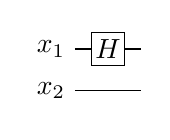
\begin{tikzpicture}[scale=1.000000,x=1pt,y=1pt]
\filldraw[color=white] (0.000000, -7.500000) rectangle (24.000000, 22.500000);
% Drawing wires
% Line 1: a2 W x_2
\draw[color=black] (0.000000,15.000000) -- (24.000000,15.000000);
\draw[color=black] (0.000000,15.000000) node[left] {$x_1$};
% Line 2: a1 W x_1
\draw[color=black] (0.000000,0.000000) -- (24.000000,0.000000);
\draw[color=black] (0.000000,0.000000) node[left] {$x_2$};
% Done with wires; drawing gates
% Line 3: a2 H
\begin{scope}
\draw[fill=white] (12.000000, 15.000000) +(-45.000000:8.485281pt and 8.485281pt) -- +(45.000000:8.485281pt and 8.485281pt) -- +(135.000000:8.485281pt and 8.485281pt) -- +(225.000000:8.485281pt and 8.485281pt) -- cycle;
\clip (12.000000, 15.000000) +(-45.000000:8.485281pt and 8.485281pt) -- +(45.000000:8.485281pt and 8.485281pt) -- +(135.000000:8.485281pt and 8.485281pt) -- +(225.000000:8.485281pt and 8.485281pt) -- cycle;
\draw (12.000000, 15.000000) node {$H$};
\end{scope}
% Done with gates; drawing ending labels
% Done with ending labels; drawing cut lines and comments
% Done with comments
\end{tikzpicture}
\end{center}
in the computation basis?  What is the unitary matrix for the circuit
\begin{center}
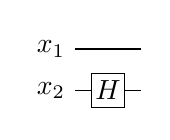
\begin{tikzpicture}[scale=1.000000,x=1pt,y=1pt]
\filldraw[color=white] (0.000000, -7.500000) rectangle (24.000000, 22.500000);
% Drawing wires
% Line 1: a2 W x_2
\draw[color=black] (0.000000,15.000000) -- (24.000000,15.000000);
\draw[color=black] (0.000000,15.000000) node[left] {$x_1$};
% Line 2: a1 W x_1
\draw[color=black] (0.000000,0.000000) -- (24.000000,0.000000);
\draw[color=black] (0.000000,0.000000) node[left] {$x_2$};
% Done with wires; drawing gates
% Line 3: a1 H
\begin{scope}
\draw[fill=white] (12.000000, -0.000000) +(-45.000000:8.485281pt and 8.485281pt) -- +(45.000000:8.485281pt and 8.485281pt) -- +(135.000000:8.485281pt and 8.485281pt) -- +(225.000000:8.485281pt and 8.485281pt) -- cycle;
\clip (12.000000, -0.000000) +(-45.000000:8.485281pt and 8.485281pt) -- +(45.000000:8.485281pt and 8.485281pt) -- +(135.000000:8.485281pt and 8.485281pt) -- +(225.000000:8.485281pt and 8.485281pt) -- cycle;
\draw (12.000000, -0.000000) node {$H$};
\end{scope}
% Done with gates; drawing ending labels
% Done with ending labels; drawing cut lines and comments
% Done with comments
\end{tikzpicture}
\end{center}
in the computational basis?
\Soln Note: we've changed the qubit labels so that reading states top to bottom corresponds to reading them left to right in the concatenated computation basis representation.   The unitary matrices are: $\frac{1}{\sqrt{2}}\begin{bmatrix} 1 & 0 & 1 & 0 \\ 0 & 1 & 0 & 1 \\ 1 & 0 & -1 & 0 \\ 0 & 1 & 0 & -1\end{bmatrix}$ and $\frac{1}{\sqrt{2}}\begin{bmatrix} 1 & 1 & 0 & 0 \\ 1 & -1 & 0 & 0 \\ 0 & 0 & 1 & 1 \\ 0 & 0 & 1 & -1\end{bmatrix}$.

\Textbf{4.17} \textbf{(Building} \CNOT \textbf{\ from controlled-$Z$ gates)} Construct a \CNOT\ gate from one controled-$Z$ gate, that is, the gate whose action in the computational basis is specified by the unitary matrix $$\begin{bmatrix} 1 & 0 & 0 &0 \\ 0 & 1 & 0 & 0 \\ 0 & 0 & 1 & 0 \\ 0 & 0 & 0 & -1\end{bmatrix},$$ and two Hadamard gates, specifying the control and target qubits. 
\Soln The Hadamard gate maps the eigenvectors of the $X$ operator to those of the $Z$ operator, so applying a Hadamard to the control before and after executing a controlled-$Z$ should effect a \CNOT.  
\begin{center}
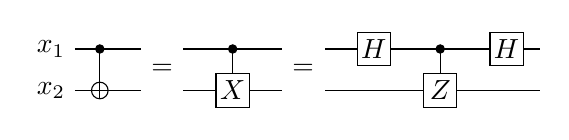
\begin{tikzpicture}[scale=1.000000,x=1pt,y=1pt]
\filldraw[color=white] (0.000000, -7.500000) rectangle (168.000000, 22.500000);
% Drawing wires
% Line 1: a2 W x_2
\draw[color=black] (0.000000,15.000000) -- (168.000000,15.000000);
\draw[color=black] (0.000000,15.000000) node[left] {$x_1$};
% Line 2: a1 W x_1
\draw[color=black] (0.000000,0.000000) -- (168.000000,0.000000);
\draw[color=black] (0.000000,0.000000) node[left] {$x_2$};
% Done with wires; drawing gates
% Line 3: +a1 a2
\draw (9.000000,15.000000) -- (9.000000,0.000000);
\begin{scope}
\draw[fill=white] (9.000000, 0.000000) circle(3.000000pt);
\clip (9.000000, 0.000000) circle(3.000000pt);
\draw (6.000000, 0.000000) -- (12.000000, 0.000000);
\draw (9.000000, -3.000000) -- (9.000000, 3.000000);
\end{scope}
\filldraw (9.000000, 15.000000) circle(1.500000pt);
% Line 4: =
\draw[fill=white,color=white] (24.000000, -6.000000) rectangle (39.000000, 21.000000);
\draw (31.500000, 7.500000) node {$=$};
% Line 5: a1 X a2
\draw (57.000000,15.000000) -- (57.000000,0.000000);
\begin{scope}
\draw[fill=white] (57.000000, -0.000000) +(-45.000000:8.485281pt and 8.485281pt) -- +(45.000000:8.485281pt and 8.485281pt) -- +(135.000000:8.485281pt and 8.485281pt) -- +(225.000000:8.485281pt and 8.485281pt) -- cycle;
\clip (57.000000, -0.000000) +(-45.000000:8.485281pt and 8.485281pt) -- +(45.000000:8.485281pt and 8.485281pt) -- +(135.000000:8.485281pt and 8.485281pt) -- +(225.000000:8.485281pt and 8.485281pt) -- cycle;
\draw (57.000000, -0.000000) node {$X$};
\end{scope}
\filldraw (57.000000, 15.000000) circle(1.500000pt);
% Line 6: =
\draw[fill=white,color=white] (75.000000, -6.000000) rectangle (90.000000, 21.000000);
\draw (82.500000, 7.500000) node {$=$};
% Line 7: a2 H
\begin{scope}
\draw[fill=white] (108.000000, 15.000000) +(-45.000000:8.485281pt and 8.485281pt) -- +(45.000000:8.485281pt and 8.485281pt) -- +(135.000000:8.485281pt and 8.485281pt) -- +(225.000000:8.485281pt and 8.485281pt) -- cycle;
\clip (108.000000, 15.000000) +(-45.000000:8.485281pt and 8.485281pt) -- +(45.000000:8.485281pt and 8.485281pt) -- +(135.000000:8.485281pt and 8.485281pt) -- +(225.000000:8.485281pt and 8.485281pt) -- cycle;
\draw (108.000000, 15.000000) node {$H$};
\end{scope}
% Line 8: a1 Z a2
\draw (132.000000,15.000000) -- (132.000000,0.000000);
\begin{scope}
\draw[fill=white] (132.000000, -0.000000) +(-45.000000:8.485281pt and 8.485281pt) -- +(45.000000:8.485281pt and 8.485281pt) -- +(135.000000:8.485281pt and 8.485281pt) -- +(225.000000:8.485281pt and 8.485281pt) -- cycle;
\clip (132.000000, -0.000000) +(-45.000000:8.485281pt and 8.485281pt) -- +(45.000000:8.485281pt and 8.485281pt) -- +(135.000000:8.485281pt and 8.485281pt) -- +(225.000000:8.485281pt and 8.485281pt) -- cycle;
\draw (132.000000, -0.000000) node {$Z$};
\end{scope}
\filldraw (132.000000, 15.000000) circle(1.500000pt);
% Line 9: a2 H
\begin{scope}
\draw[fill=white] (156.000000, 15.000000) +(-45.000000:8.485281pt and 8.485281pt) -- +(45.000000:8.485281pt and 8.485281pt) -- +(135.000000:8.485281pt and 8.485281pt) -- +(225.000000:8.485281pt and 8.485281pt) -- cycle;
\clip (156.000000, 15.000000) +(-45.000000:8.485281pt and 8.485281pt) -- +(45.000000:8.485281pt and 8.485281pt) -- +(135.000000:8.485281pt and 8.485281pt) -- +(225.000000:8.485281pt and 8.485281pt) -- cycle;
\draw (156.000000, 15.000000) node {$H$};
\end{scope}
% Done with gates; drawing ending labels
% Done with ending labels; drawing cut lines and comments
% Done with comments
\end{tikzpicture}
\end{center}
In matrix form, this corresponds to $$\begin{bmatrix} 1 & 0 & 0 & 0 \\ 0 & 1 & 0 & 0 \\ 0 & 0 & 0 & 1 \\ 0 & 0 & 1 & 0 \end{bmatrix} = \frac{1}{2}\begin{bmatrix} 1 & 0 & 1 & 0 \\ 0 & 1 & 0 & 1 \\ 1 & 0 & -1 & 0 \\ 0 & 1 & 0 & -1\end{bmatrix}\begin{bmatrix} 1 & 0 & 0 &0 \\ 0 & 1 & 0 & 0 \\ 0 & 0 & 1 & 0 \\ 0 & 0 & 0 & -1\end{bmatrix}\begin{bmatrix} 1 & 0 & 1 & 0 \\ 0 & 1 & 0 & 1 \\ 1 & 0 & -1 & 0 \\ 0 & 1 & 0 & -1\end{bmatrix}.$$

\Textbf{4.18} Show that 
\begin{center}
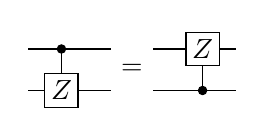
\begin{tikzpicture}[scale=1.000000,x=1pt,y=1pt]
\filldraw[color=white] (0.000000, -7.500000) rectangle (75.000000, 22.500000);
% Drawing wires
% Line 1: a2 W
\draw[color=black] (0.000000,15.000000) -- (75.000000,15.000000);
% Line 2: a1 W
\draw[color=black] (0.000000,0.000000) -- (75.000000,0.000000);
% Done with wires; drawing gates
% Line 3: a1 Z a2
\draw (12.000000,15.000000) -- (12.000000,0.000000);
\begin{scope}
\draw[fill=white] (12.000000, -0.000000) +(-45.000000:8.485281pt and 8.485281pt) -- +(45.000000:8.485281pt and 8.485281pt) -- +(135.000000:8.485281pt and 8.485281pt) -- +(225.000000:8.485281pt and 8.485281pt) -- cycle;
\clip (12.000000, -0.000000) +(-45.000000:8.485281pt and 8.485281pt) -- +(45.000000:8.485281pt and 8.485281pt) -- +(135.000000:8.485281pt and 8.485281pt) -- +(225.000000:8.485281pt and 8.485281pt) -- cycle;
\draw (12.000000, -0.000000) node {$Z$};
\end{scope}
\filldraw (12.000000, 15.000000) circle(1.500000pt);
% Line 4: =
\draw[fill=white,color=white] (30.000000, -6.000000) rectangle (45.000000, 21.000000);
\draw (37.500000, 7.500000) node {$=$};
% Line 5: a2 Z a1
\draw (63.000000,15.000000) -- (63.000000,0.000000);
\begin{scope}
\draw[fill=white] (63.000000, 15.000000) +(-45.000000:8.485281pt and 8.485281pt) -- +(45.000000:8.485281pt and 8.485281pt) -- +(135.000000:8.485281pt and 8.485281pt) -- +(225.000000:8.485281pt and 8.485281pt) -- cycle;
\clip (63.000000, 15.000000) +(-45.000000:8.485281pt and 8.485281pt) -- +(45.000000:8.485281pt and 8.485281pt) -- +(135.000000:8.485281pt and 8.485281pt) -- +(225.000000:8.485281pt and 8.485281pt) -- cycle;
\draw (63.000000, 15.000000) node {$Z$};
\end{scope}
\filldraw (63.000000, 0.000000) circle(1.500000pt);
% Done with gates; drawing ending labels
% Done with ending labels; drawing cut lines and comments
% Done with comments
\end{tikzpicture}
\end{center}
\Soln In the computational basis the controlled-$Z$ changes the state if and only if the control and target qubits are both $\ket{1}$.  In this criteria the control and target are interchangeable, so these gates perform the same action.
\newpage
\Textbf{4.19} \textbf{(}\CNOT\ \textbf{action on density matrices)} The \CNOT\ gate is a simple permutation whose action on a density matrix $\rho$ is to rearrange the elements in the matrix. Write out this action explicitly in the computational basis.
\Soln $$\ket{x_2x_1} = \alpha\ket{00}+\beta\ket{01}+\gamma\ket{10}+\delta\ket{11} \xrightarrow[]{CX} \alpha\ket{00}+\beta\ket{01}+\underline{\delta}\ket{10}+\underline{\gamma}\ket{11}.$$

\Textbf{4.20} \textbf{(}\CNOT\ \textbf{basis transformation)} Unlike ideal classical gates, ideal quantum gates do not have (as electrical engineers say) `high-impedence' inputs.  In fact, the role of `control' and `target' are arbitrary -- they depend on what basis you think of a device as operating in.  We have described how the \CNOT\ behaves with respect to the computational basis, and in this description the state of the control qubit is not changed.  However, if we work in a different basis then the control qubit \textit{does} change: we will show that its phase is flipped depending on the state of the `target' qubit!  Show that
\begin{center}
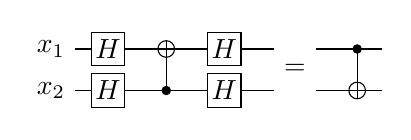
\begin{tikzpicture}[scale=1.000000,x=1pt,y=1pt]
\filldraw[color=white] (0.000000, -7.500000) rectangle (111.000000, 22.500000);
% Drawing wires
% Line 1: a1 W $x_1$
\draw[color=black] (0.000000,15.000000) -- (111.000000,15.000000);
\draw[color=black] (0.000000,15.000000) node[left] {$x_1$};
% Line 2: a2 W $x_2$
\draw[color=black] (0.000000,0.000000) -- (111.000000,0.000000);
\draw[color=black] (0.000000,0.000000) node[left] {$x_2$};
% Done with wires; drawing gates
% Line 3: a1 H
\begin{scope}
\draw[fill=white] (12.000000, 15.000000) +(-45.000000:8.485281pt and 8.485281pt) -- +(45.000000:8.485281pt and 8.485281pt) -- +(135.000000:8.485281pt and 8.485281pt) -- +(225.000000:8.485281pt and 8.485281pt) -- cycle;
\clip (12.000000, 15.000000) +(-45.000000:8.485281pt and 8.485281pt) -- +(45.000000:8.485281pt and 8.485281pt) -- +(135.000000:8.485281pt and 8.485281pt) -- +(225.000000:8.485281pt and 8.485281pt) -- cycle;
\draw (12.000000, 15.000000) node {$H$};
\end{scope}
% Line 4: a2 H
\begin{scope}
\draw[fill=white] (12.000000, -0.000000) +(-45.000000:8.485281pt and 8.485281pt) -- +(45.000000:8.485281pt and 8.485281pt) -- +(135.000000:8.485281pt and 8.485281pt) -- +(225.000000:8.485281pt and 8.485281pt) -- cycle;
\clip (12.000000, -0.000000) +(-45.000000:8.485281pt and 8.485281pt) -- +(45.000000:8.485281pt and 8.485281pt) -- +(135.000000:8.485281pt and 8.485281pt) -- +(225.000000:8.485281pt and 8.485281pt) -- cycle;
\draw (12.000000, -0.000000) node {$H$};
\end{scope}
% Line 5: +a1 a2
\draw (33.000000,15.000000) -- (33.000000,0.000000);
\begin{scope}
\draw[fill=white] (33.000000, 15.000000) circle(3.000000pt);
\clip (33.000000, 15.000000) circle(3.000000pt);
\draw (30.000000, 15.000000) -- (36.000000, 15.000000);
\draw (33.000000, 12.000000) -- (33.000000, 18.000000);
\end{scope}
\filldraw (33.000000, 0.000000) circle(1.500000pt);
% Line 6: a1 H
\begin{scope}
\draw[fill=white] (54.000000, 15.000000) +(-45.000000:8.485281pt and 8.485281pt) -- +(45.000000:8.485281pt and 8.485281pt) -- +(135.000000:8.485281pt and 8.485281pt) -- +(225.000000:8.485281pt and 8.485281pt) -- cycle;
\clip (54.000000, 15.000000) +(-45.000000:8.485281pt and 8.485281pt) -- +(45.000000:8.485281pt and 8.485281pt) -- +(135.000000:8.485281pt and 8.485281pt) -- +(225.000000:8.485281pt and 8.485281pt) -- cycle;
\draw (54.000000, 15.000000) node {$H$};
\end{scope}
% Line 7: a2 H
\begin{scope}
\draw[fill=white] (54.000000, -0.000000) +(-45.000000:8.485281pt and 8.485281pt) -- +(45.000000:8.485281pt and 8.485281pt) -- +(135.000000:8.485281pt and 8.485281pt) -- +(225.000000:8.485281pt and 8.485281pt) -- cycle;
\clip (54.000000, -0.000000) +(-45.000000:8.485281pt and 8.485281pt) -- +(45.000000:8.485281pt and 8.485281pt) -- +(135.000000:8.485281pt and 8.485281pt) -- +(225.000000:8.485281pt and 8.485281pt) -- cycle;
\draw (54.000000, -0.000000) node {$H$};
\end{scope}
% Line 8: =
\draw[fill=white,color=white] (72.000000, -6.000000) rectangle (87.000000, 21.000000);
\draw (79.500000, 7.500000) node {$=$};
% Line 9: a1 +a2
\draw (102.000000,15.000000) -- (102.000000,0.000000);
\filldraw (102.000000, 15.000000) circle(1.500000pt);
\begin{scope}
\draw[fill=white] (102.000000, 0.000000) circle(3.000000pt);
\clip (102.000000, 0.000000) circle(3.000000pt);
\draw (99.000000, 0.000000) -- (105.000000, 0.000000);
\draw (102.000000, -3.000000) -- (102.000000, 3.000000);
\end{scope}
% Done with gates; drawing ending labels
% Done with ending labels; drawing cut lines and comments
% Done with comments
\end{tikzpicture}
\end{center}
Introducing basis states $\ket{\pm}\equiv(\ket{0}\pm\ket{1})/\sqrt{2}$, use this circuit identity to show that the effect of a \CNOT\ with the first qubit as control and the second qubit as target is as follows:
\begin{align*}
\ket{x_1}\ket{x_2}& \\
\ket{+}\ket{+}&\rightarrow\ket{+}\ket{+}\\
\ket{-}\ket{+}&\rightarrow\ket{-}\ket{+}\\
\ket{+}\ket{-}&\rightarrow\ket{-}\ket{-}\\
\ket{-}\ket{-}&\rightarrow\ket{+}\ket{-}.
\end{align*}
Thus, with respect to the this new basis, the state of the target qubit is not changed, while the state of the control qubit is flipped if the target starts as $\ket{-}$, otherwise it is left alone. That is, in this basis, the target and control have essentially interchanged roles!
\Soln Note, we've switched the roles of qubits in the diagram (and labeled them)  so that reading states top to bottom in the diagram corresponds to reading them left to right in the concatenated basis representation.  To show the circuit identity, we use matrix multiplication:
$$\frac{1}{4} \begin{bmatrix} 1 & 1 & 0 & 0 \\ 1 & -1 & 0 & 0 \\ 0 & 0 & 1 & 1 \\ 0 & 0 & 1 & -1\end{bmatrix}\begin{bmatrix} 1 & 0 & 1 & 0 \\ 0 & 1 & 0 & 1 \\ 1 & 0 & -1 & 0 \\ 0 & 1 & 0 & -1\end{bmatrix} \begin{bmatrix} 1 & 0 & 0 &0 \\ 0 & 0 & 0 & 1 \\ 0 & 0 & 1 & 0 \\ 0 & 1 & 0 & 0\end{bmatrix}\begin{bmatrix} 1 & 1 & 0 & 0 \\ 1 & -1 & 0 & 0 \\ 0 & 0 & 1 & 1 \\ 0 & 0 & 1 & -1\end{bmatrix}\begin{bmatrix} 1 & 0 & 1 & 0 \\ 0 & 1 & 0 & 1 \\ 1 & 0 & -1 & 0 \\ 0 & 1 & 0 & -1\end{bmatrix} =\begin{bmatrix} 1 & 0 & 0 &0 \\ 0 & 1 & 0 & 0 \\ 0 & 0 & 0 & 1 \\ 0 & 0 & 1 & 0\end{bmatrix}.$$
\vspace{-15pt}
\begin{center}\ \ \ \ $H(x_1,\_)$ \quad\quad\quad\quad $H(\_, x_2)$  \quad\quad \CNOT$(x_2,x_1)$ \quad\quad $H(x_1,\_)$ \quad\quad\quad $H(\_, x_2)$ \quad\quad\quad \CNOT$(x_1,x_2)$ \end{center}
The matrix in the middle on the left can be verified to be the representation of the action of \CNOT\ in the computational basis, with $x_2$ as control, and $x_1$  as target.  In functional notation below, we'll let \CNOT$(x_1, x_2)$ denote the action of a \CNOT\ controlled by $\ket{x_1}$ and targetting $\ket{x_2}$, with \CNOT$'(x_1,x_2) \equiv$ \CNOT$(x_2,x_1)$ switching target and control, and let $H(x_1, x_2)$ denote the application of Hadamard gates to both qubits.  The circuit identity is that $H($\CNOT$'(H(x_1, x_2)) =\ $\CNOT$(x_1,x_2)$.  Now:

\begin{center}
\textcolor{white}{\CNOT}$(\ket{x_1},\ket{x_2})$\textcolor{white}{$ = H($\CNOT$''(H(\ket{+},\ket{+}))) = H($\CNOT$'(\ket{0},\ket{0})) = H(\ket{0},\ket{0}) = \ket{+}\ket{+}$}
\CNOT$(\ket{+},\ket{+}) = H($\CNOT$'(H(\ket{+},\ket{+}))) = H($\CNOT$'(\ket{0},\ket{0})) = H(\ket{0},\ket{0}) = \ket{+}\ket{+}$
\CNOT$(\ket{-},\ket{+}) = H($\CNOT$'(H(\ket{-},\ket{+}))) = H($\CNOT$'(\ket{1},\ket{0})) = H(\ket{1},\ket{0}) = \ket{-}\ket{+}$ % This isn't right, I can't keep track of the endianess
\CNOT$(\ket{+},\ket{-}) = H($\CNOT$'(H(\ket{+},\ket{-}))) = H($\CNOT$'(\ket{0},\ket{1})) = H(\ket{1},\ket{1}) = \ket{-}\ket{-}$
\CNOT$(\ket{-},\ket{-}) = H($\CNOT$'(H(\ket{-},\ket{-}))) = H($\CNOT$'(\ket{1},\ket{1})) = H(\ket{0},\ket{1}) = \ket{+}\ket{-}$ % This isn't right, I can't keep track of the endianess
\end{center}
\Textbf{4.21} Suppose $U$ is a single qubit unitary operator, and $V$ is a unitary operator chosen so that $V^2=U$.  Verify that Figure 4.8 implements the $C^2(U)$ operation.
\begin{center}
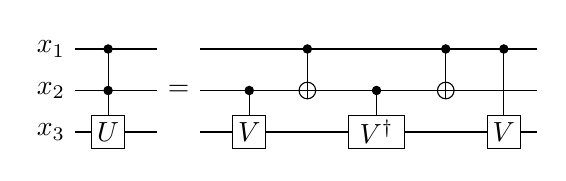
\begin{tikzpicture}[scale=1.000000,x=1pt,y=1pt]
\filldraw[color=white] (0.000000, -7.500000) rectangle (167.000000, 37.500000);
% Drawing wires
% Line 1: a3 W x_3
\draw[color=black] (0.000000,30.000000) -- (167.000000,30.000000);
\draw[color=black] (0.000000,30.000000) node[left] {$x_1$};
% Line 2: a2 W x_2
\draw[color=black] (0.000000,15.000000) -- (167.000000,15.000000);
\draw[color=black] (0.000000,15.000000) node[left] {$x_2$};
% Line 3: a1 W x_1
\draw[color=black] (0.000000,0.000000) -- (167.000000,0.000000);
\draw[color=black] (0.000000,0.000000) node[left] {$x_3$};
% Done with wires; drawing gates
% Line 4: a1 G $U$ a2 a3
\draw (12.000000,30.000000) -- (12.000000,0.000000);
\begin{scope}
\draw[fill=white] (12.000000, -0.000000) +(-45.000000:8.485281pt and 8.485281pt) -- +(45.000000:8.485281pt and 8.485281pt) -- +(135.000000:8.485281pt and 8.485281pt) -- +(225.000000:8.485281pt and 8.485281pt) -- cycle;
\clip (12.000000, -0.000000) +(-45.000000:8.485281pt and 8.485281pt) -- +(45.000000:8.485281pt and 8.485281pt) -- +(135.000000:8.485281pt and 8.485281pt) -- +(225.000000:8.485281pt and 8.485281pt) -- cycle;
\draw (12.000000, -0.000000) node {$U$};
\end{scope}
\filldraw (12.000000, 15.000000) circle(1.500000pt);
\filldraw (12.000000, 30.000000) circle(1.500000pt);
% Line 5: =
\draw[fill=white,color=white] (30.000000, -6.000000) rectangle (45.000000, 36.000000);
\draw (37.500000, 15.000000) node {$=$};
% Line 6: a1 G $V$ a2
\draw (63.000000,15.000000) -- (63.000000,0.000000);
\begin{scope}
\draw[fill=white] (63.000000, -0.000000) +(-45.000000:8.485281pt and 8.485281pt) -- +(45.000000:8.485281pt and 8.485281pt) -- +(135.000000:8.485281pt and 8.485281pt) -- +(225.000000:8.485281pt and 8.485281pt) -- cycle;
\clip (63.000000, -0.000000) +(-45.000000:8.485281pt and 8.485281pt) -- +(45.000000:8.485281pt and 8.485281pt) -- +(135.000000:8.485281pt and 8.485281pt) -- +(225.000000:8.485281pt and 8.485281pt) -- cycle;
\draw (63.000000, -0.000000) node {$V$};
\end{scope}
\filldraw (63.000000, 15.000000) circle(1.500000pt);
% Line 7: +a2 a3
\draw (84.000000,30.000000) -- (84.000000,15.000000);
\begin{scope}
\draw[fill=white] (84.000000, 15.000000) circle(3.000000pt);
\clip (84.000000, 15.000000) circle(3.000000pt);
\draw (81.000000, 15.000000) -- (87.000000, 15.000000);
\draw (84.000000, 12.000000) -- (84.000000, 18.000000);
\end{scope}
\filldraw (84.000000, 30.000000) circle(1.500000pt);
% Line 8: a1 G $V^\dagger$ a2 width=20
\draw (109.000000,15.000000) -- (109.000000,0.000000);
\begin{scope}
\draw[fill=white] (109.000000, -0.000000) +(-45.000000:14.142136pt and 8.485281pt) -- +(45.000000:14.142136pt and 8.485281pt) -- +(135.000000:14.142136pt and 8.485281pt) -- +(225.000000:14.142136pt and 8.485281pt) -- cycle;
\clip (109.000000, -0.000000) +(-45.000000:14.142136pt and 8.485281pt) -- +(45.000000:14.142136pt and 8.485281pt) -- +(135.000000:14.142136pt and 8.485281pt) -- +(225.000000:14.142136pt and 8.485281pt) -- cycle;
\draw (109.000000, -0.000000) node {$V^\dagger$};
\end{scope}
\filldraw (109.000000, 15.000000) circle(1.500000pt);
% Line 9: +a2 a3
\draw (134.000000,30.000000) -- (134.000000,15.000000);
\begin{scope}
\draw[fill=white] (134.000000, 15.000000) circle(3.000000pt);
\clip (134.000000, 15.000000) circle(3.000000pt);
\draw (131.000000, 15.000000) -- (137.000000, 15.000000);
\draw (134.000000, 12.000000) -- (134.000000, 18.000000);
\end{scope}
\filldraw (134.000000, 30.000000) circle(1.500000pt);
% Line 10: a1 G $V$ a3
\draw (155.000000,30.000000) -- (155.000000,0.000000);
\begin{scope}
\draw[fill=white] (155.000000, -0.000000) +(-45.000000:8.485281pt and 8.485281pt) -- +(45.000000:8.485281pt and 8.485281pt) -- +(135.000000:8.485281pt and 8.485281pt) -- +(225.000000:8.485281pt and 8.485281pt) -- cycle;
\clip (155.000000, -0.000000) +(-45.000000:8.485281pt and 8.485281pt) -- +(45.000000:8.485281pt and 8.485281pt) -- +(135.000000:8.485281pt and 8.485281pt) -- +(225.000000:8.485281pt and 8.485281pt) -- cycle;
\draw (155.000000, -0.000000) node {$V$};
\end{scope}
\filldraw (155.000000, 30.000000) circle(1.500000pt);
% Done with gates; drawing ending labels
% Done with ending labels; drawing cut lines and comments
% Done with comments
\end{tikzpicture}
\end{center}
\vspace{-15pt}
\Soln We verify by tracking the applications of $V$ and $V^\dagger$ to $\ket{x_3}$ for each computational basis state representing $\ket{x_1}\ket{x_2}$.  The first $V$ is applied when $\ket{x_2}=\ket{1}$.  The first \CNOT\ calculates the parity of $\ket{x_1}\ket{x_2}$ so that the middle $V^\dagger$ is applied for when $\ket{x_1}\ket{x_2} = \ket{0}\ket{1}\ \mathrm{or}\ \ket{1}\ket{0}$.  The second \CNOT\ uncomputes the parity  so that in the end $\ket{x_1}\ket{x_2}$ is unchanged.  The final $V$ is then applied if $\ket{x_1}=\ket{1}$.  In the end, the output of the circuit is
\begin{align*}
\ket{x_1}\ket{x_2}\ \ \ \ \\
\ket{0}\ket{0}\ket{x_3}\ &\rightarrow \ket{0}\ket{0}\ \ \ \ \ \ \ \ket{x_3} \\
\ket{0}\ket{1}\ket{x_3}\ &\rightarrow\ket{0}\ket{1}VV^\dagger\ket{x_3} =\ket{0}\ket{1}\ \ \ \ket{x_3} \tag{$V$ is unitary, $VV^\dagger=I$}\\
\ket{1}\ket{0}\ket{x_3}\ &\rightarrow\ket{1}\ket{0} V^\dagger V\ket{x_3} = \ket{1}\ket{0}\ \ \ \ket{x_3} \tag{$V$ is unitary, $V^\dagger V=I$}\\
\ket{1}\ket{1}\ket{x_3}\ &\rightarrow \ket{1}\ket{1}\ \ V^2\ket{x_3}=\ket{1}\ket{1} U\ket{x_3} \tag{$   V^2=U$}
\end{align*}

\Textbf{4.22} Prove that a $C^2(U)$ gate (for any single qubit unitary $U$) can be constructed using at most eight one-qubit gates, and six controlled-\NOT s
\Soln Note: this solution borrows heavily from  DaftWullie's answer to the quantumcomputing.stackexhange question here: \href{_}\url{https://quantumcomputing.stackexchange.com/questions/7082/how-to-reduce-circuit-elements-of-a-decomposed-c2u-operation}.

 Let $V$ be a single-qubit unitary operator such that $V^2=U$, and By Corollary 4.2, let $A,B,$ and $C$ be single-qubit unitary operators and $\alpha$ an overall phase factor such that $ABC=I$ and $V=e^{i\alpha}AXBXC$. Combining figures 4.6 and 4.8 gives

\begin{center}
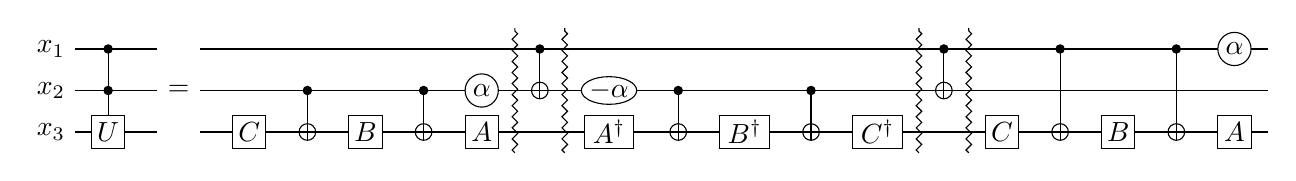
\begin{tikzpicture}[scale=1.000000,x=1pt,y=1pt]
\filldraw[color=white] (0.000000, -7.500000) rectangle (431.000000, 37.500000);
% Drawing wires
% Line 1: a3 W x_3
\draw[color=black] (0.000000,30.000000) -- (431.000000,30.000000);
\draw[color=black] (0.000000,30.000000) node[left] {$x_1$};
% Line 2: a2 W x_2
\draw[color=black] (0.000000,15.000000) -- (431.000000,15.000000);
\draw[color=black] (0.000000,15.000000) node[left] {$x_2$};
% Line 3: a1 W x_1
\draw[color=black] (0.000000,0.000000) -- (431.000000,0.000000);
\draw[color=black] (0.000000,0.000000) node[left] {$x_3$};
% Done with wires; drawing gates
% Line 4: a1 G $U$ a2 a3
\draw (12.000000,30.000000) -- (12.000000,0.000000);
\begin{scope}
\draw[fill=white] (12.000000, -0.000000) +(-45.000000:8.485281pt and 8.485281pt) -- +(45.000000:8.485281pt and 8.485281pt) -- +(135.000000:8.485281pt and 8.485281pt) -- +(225.000000:8.485281pt and 8.485281pt) -- cycle;
\clip (12.000000, -0.000000) +(-45.000000:8.485281pt and 8.485281pt) -- +(45.000000:8.485281pt and 8.485281pt) -- +(135.000000:8.485281pt and 8.485281pt) -- +(225.000000:8.485281pt and 8.485281pt) -- cycle;
\draw (12.000000, -0.000000) node {$U$};
\end{scope}
\filldraw (12.000000, 15.000000) circle(1.500000pt);
\filldraw (12.000000, 30.000000) circle(1.500000pt);
% Line 5: =
\draw[fill=white,color=white] (30.000000, -6.000000) rectangle (45.000000, 36.000000);
\draw (37.500000, 15.000000) node {$=$};
% Line 6: a1 G $C$
\begin{scope}
\draw[fill=white] (63.000000, -0.000000) +(-45.000000:8.485281pt and 8.485281pt) -- +(45.000000:8.485281pt and 8.485281pt) -- +(135.000000:8.485281pt and 8.485281pt) -- +(225.000000:8.485281pt and 8.485281pt) -- cycle;
\clip (63.000000, -0.000000) +(-45.000000:8.485281pt and 8.485281pt) -- +(45.000000:8.485281pt and 8.485281pt) -- +(135.000000:8.485281pt and 8.485281pt) -- +(225.000000:8.485281pt and 8.485281pt) -- cycle;
\draw (63.000000, -0.000000) node {$C$};
\end{scope}
% Line 7: +a1 a2
\draw (84.000000,15.000000) -- (84.000000,0.000000);
\begin{scope}
\draw[fill=white] (84.000000, 0.000000) circle(3.000000pt);
\clip (84.000000, 0.000000) circle(3.000000pt);
\draw (81.000000, 0.000000) -- (87.000000, 0.000000);
\draw (84.000000, -3.000000) -- (84.000000, 3.000000);
\end{scope}
\filldraw (84.000000, 15.000000) circle(1.500000pt);
% Line 8: a1 G $B$
\begin{scope}
\draw[fill=white] (105.000000, -0.000000) +(-45.000000:8.485281pt and 8.485281pt) -- +(45.000000:8.485281pt and 8.485281pt) -- +(135.000000:8.485281pt and 8.485281pt) -- +(225.000000:8.485281pt and 8.485281pt) -- cycle;
\clip (105.000000, -0.000000) +(-45.000000:8.485281pt and 8.485281pt) -- +(45.000000:8.485281pt and 8.485281pt) -- +(135.000000:8.485281pt and 8.485281pt) -- +(225.000000:8.485281pt and 8.485281pt) -- cycle;
\draw (105.000000, -0.000000) node {$B$};
\end{scope}
% Line 9: +a1 a2
\draw (126.000000,15.000000) -- (126.000000,0.000000);
\begin{scope}
\draw[fill=white] (126.000000, 0.000000) circle(3.000000pt);
\clip (126.000000, 0.000000) circle(3.000000pt);
\draw (123.000000, 0.000000) -- (129.000000, 0.000000);
\draw (126.000000, -3.000000) -- (126.000000, 3.000000);
\end{scope}
\filldraw (126.000000, 15.000000) circle(1.500000pt);
% Line 10: a2 P $\alpha$
\begin{scope}
\draw[fill=white] (147.000000, 15.000000) circle(6.000000pt);
\clip (147.000000, 15.000000) circle(6.000000pt);
\draw (147.000000, 15.000000) node {$\alpha$};
\end{scope}
% Line 11: a1 G $A$
\begin{scope}
\draw[fill=white] (147.000000, -0.000000) +(-45.000000:8.485281pt and 8.485281pt) -- +(45.000000:8.485281pt and 8.485281pt) -- +(135.000000:8.485281pt and 8.485281pt) -- +(225.000000:8.485281pt and 8.485281pt) -- cycle;
\clip (147.000000, -0.000000) +(-45.000000:8.485281pt and 8.485281pt) -- +(45.000000:8.485281pt and 8.485281pt) -- +(135.000000:8.485281pt and 8.485281pt) -- +(225.000000:8.485281pt and 8.485281pt) -- cycle;
\draw (147.000000, -0.000000) node {$A$};
\end{scope}
% Line 12: a3 a2 a1 BARRIER
\draw[decorate,decoration={zigzag,amplitude=1pt,segment length=4}] (159.000000,-7.500000) -- (159.000000,37.500000);
% Line 13: +a2 a3
\draw (168.000000,30.000000) -- (168.000000,15.000000);
\begin{scope}
\draw[fill=white] (168.000000, 15.000000) circle(3.000000pt);
\clip (168.000000, 15.000000) circle(3.000000pt);
\draw (165.000000, 15.000000) -- (171.000000, 15.000000);
\draw (168.000000, 12.000000) -- (168.000000, 18.000000);
\end{scope}
\filldraw (168.000000, 30.000000) circle(1.500000pt);
% Line 14: a3 a2 a1 BARRIER
\draw[decorate,decoration={zigzag,amplitude=1pt,segment length=4}] (177.000000,-7.500000) -- (177.000000,37.500000);
% Line 16: a1 G $A^\dagger$ width=18
\begin{scope}
\draw[fill=white] (193.000000, -0.000000) +(-45.000000:12.727922pt and 8.485281pt) -- +(45.000000:12.727922pt and 8.485281pt) -- +(135.000000:12.727922pt and 8.485281pt) -- +(225.000000:12.727922pt and 8.485281pt) -- cycle;
\clip (193.000000, -0.000000) +(-45.000000:12.727922pt and 8.485281pt) -- +(45.000000:12.727922pt and 8.485281pt) -- +(135.000000:12.727922pt and 8.485281pt) -- +(225.000000:12.727922pt and 8.485281pt) -- cycle;
\draw (193.000000, -0.000000) node {$A^\dagger$};
\end{scope}
% Line 17: a2 P $-\alpha$ height=10 width=20
\begin{scope}
\draw[fill=white] (193.000000, 15.000000) ellipse(10.000000pt and 5.000000pt);
\clip (193.000000, 15.000000) ellipse(10.000000pt and 5.000000pt);
\draw (193.000000, 15.000000) node {$-\alpha$};
\end{scope}
% Line 18: +a1 a2
\draw (218.000000,15.000000) -- (218.000000,0.000000);
\begin{scope}
\draw[fill=white] (218.000000, 0.000000) circle(3.000000pt);
\clip (218.000000, 0.000000) circle(3.000000pt);
\draw (215.000000, 0.000000) -- (221.000000, 0.000000);
\draw (218.000000, -3.000000) -- (218.000000, 3.000000);
\end{scope}
\filldraw (218.000000, 15.000000) circle(1.500000pt);
% Line 19: a1 G $B^\dagger$ width=18
\begin{scope}
\draw[fill=white] (242.000000, -0.000000) +(-45.000000:12.727922pt and 8.485281pt) -- +(45.000000:12.727922pt and 8.485281pt) -- +(135.000000:12.727922pt and 8.485281pt) -- +(225.000000:12.727922pt and 8.485281pt) -- cycle;
\clip (242.000000, -0.000000) +(-45.000000:12.727922pt and 8.485281pt) -- +(45.000000:12.727922pt and 8.485281pt) -- +(135.000000:12.727922pt and 8.485281pt) -- +(225.000000:12.727922pt and 8.485281pt) -- cycle;
\draw (242.000000, -0.000000) node {$B^\dagger$};
\end{scope}
% Line 20: +a1 a2
\draw (266.000000,15.000000) -- (266.000000,0.000000);
\begin{scope}
\draw[fill=white] (266.000000, 0.000000) circle(3.000000pt);
\clip (266.000000, 0.000000) circle(3.000000pt);
\draw (263.000000, 0.000000) -- (269.000000, 0.000000);
\draw (266.000000, -3.000000) -- (266.000000, 3.000000);
\end{scope}
\filldraw (266.000000, 15.000000) circle(1.500000pt);
% Line 21: a1 G $C^\dagger$ width=18
\begin{scope}
\draw[fill=white] (290.000000, -0.000000) +(-45.000000:12.727922pt and 8.485281pt) -- +(45.000000:12.727922pt and 8.485281pt) -- +(135.000000:12.727922pt and 8.485281pt) -- +(225.000000:12.727922pt and 8.485281pt) -- cycle;
\clip (290.000000, -0.000000) +(-45.000000:12.727922pt and 8.485281pt) -- +(45.000000:12.727922pt and 8.485281pt) -- +(135.000000:12.727922pt and 8.485281pt) -- +(225.000000:12.727922pt and 8.485281pt) -- cycle;
\draw (290.000000, -0.000000) node {$C^\dagger$};
\end{scope}
% Line 22: a3 a2 a1 BARRIER
\draw[decorate,decoration={zigzag,amplitude=1pt,segment length=4}] (305.000000,-7.500000) -- (305.000000,37.500000);
% Line 23: +a2 a3
\draw (314.000000,30.000000) -- (314.000000,15.000000);
\begin{scope}
\draw[fill=white] (314.000000, 15.000000) circle(3.000000pt);
\clip (314.000000, 15.000000) circle(3.000000pt);
\draw (311.000000, 15.000000) -- (317.000000, 15.000000);
\draw (314.000000, 12.000000) -- (314.000000, 18.000000);
\end{scope}
\filldraw (314.000000, 30.000000) circle(1.500000pt);
% Line 24: a3 a2 a1 BARRIER
\draw[decorate,decoration={zigzag,amplitude=1pt,segment length=4}] (323.000000,-7.500000) -- (323.000000,37.500000);
% Line 25: a1 G $C$
\begin{scope}
\draw[fill=white] (335.000000, -0.000000) +(-45.000000:8.485281pt and 8.485281pt) -- +(45.000000:8.485281pt and 8.485281pt) -- +(135.000000:8.485281pt and 8.485281pt) -- +(225.000000:8.485281pt and 8.485281pt) -- cycle;
\clip (335.000000, -0.000000) +(-45.000000:8.485281pt and 8.485281pt) -- +(45.000000:8.485281pt and 8.485281pt) -- +(135.000000:8.485281pt and 8.485281pt) -- +(225.000000:8.485281pt and 8.485281pt) -- cycle;
\draw (335.000000, -0.000000) node {$C$};
\end{scope}
% Line 26: +a1 a3
\draw (356.000000,30.000000) -- (356.000000,0.000000);
\begin{scope}
\draw[fill=white] (356.000000, 0.000000) circle(3.000000pt);
\clip (356.000000, 0.000000) circle(3.000000pt);
\draw (353.000000, 0.000000) -- (359.000000, 0.000000);
\draw (356.000000, -3.000000) -- (356.000000, 3.000000);
\end{scope}
\filldraw (356.000000, 30.000000) circle(1.500000pt);
% Line 27: a1 G $B$
\begin{scope}
\draw[fill=white] (377.000000, -0.000000) +(-45.000000:8.485281pt and 8.485281pt) -- +(45.000000:8.485281pt and 8.485281pt) -- +(135.000000:8.485281pt and 8.485281pt) -- +(225.000000:8.485281pt and 8.485281pt) -- cycle;
\clip (377.000000, -0.000000) +(-45.000000:8.485281pt and 8.485281pt) -- +(45.000000:8.485281pt and 8.485281pt) -- +(135.000000:8.485281pt and 8.485281pt) -- +(225.000000:8.485281pt and 8.485281pt) -- cycle;
\draw (377.000000, -0.000000) node {$B$};
\end{scope}
% Line 28: +a1 a3
\draw (398.000000,30.000000) -- (398.000000,0.000000);
\begin{scope}
\draw[fill=white] (398.000000, 0.000000) circle(3.000000pt);
\clip (398.000000, 0.000000) circle(3.000000pt);
\draw (395.000000, 0.000000) -- (401.000000, 0.000000);
\draw (398.000000, -3.000000) -- (398.000000, 3.000000);
\end{scope}
\filldraw (398.000000, 30.000000) circle(1.500000pt);
% Line 29: a3 P $\alpha$
\begin{scope}
\draw[fill=white] (419.000000, 30.000000) circle(6.000000pt);
\clip (419.000000, 30.000000) circle(6.000000pt);
\draw (419.000000, 30.000000) node {$\alpha$};
\end{scope}
% Line 30: a1 G $A$
\begin{scope}
\draw[fill=white] (419.000000, -0.000000) +(-45.000000:8.485281pt and 8.485281pt) -- +(45.000000:8.485281pt and 8.485281pt) -- +(135.000000:8.485281pt and 8.485281pt) -- +(225.000000:8.485281pt and 8.485281pt) -- cycle;
\clip (419.000000, -0.000000) +(-45.000000:8.485281pt and 8.485281pt) -- +(45.000000:8.485281pt and 8.485281pt) -- +(135.000000:8.485281pt and 8.485281pt) -- +(225.000000:8.485281pt and 8.485281pt) -- cycle;
\draw (419.000000, -0.000000) node {$A$};
\end{scope}
% Done with gates; drawing ending labels
% Done with ending labels; drawing cut lines and comments
% Done with comments
\end{tikzpicture}
\end{center}
\vspace{-10pt}
where the \encircle{$\pm\alpha$} gates correspond to the action of $\begin{bmatrix} 1 & 0 \\ 0 & e^{\pm i\alpha}\end{bmatrix}$.  The $AA^{\dagger}$ and the $C^\dagger C$ cancel, each resulting in the identity, so we arrive at:
\begin{center}
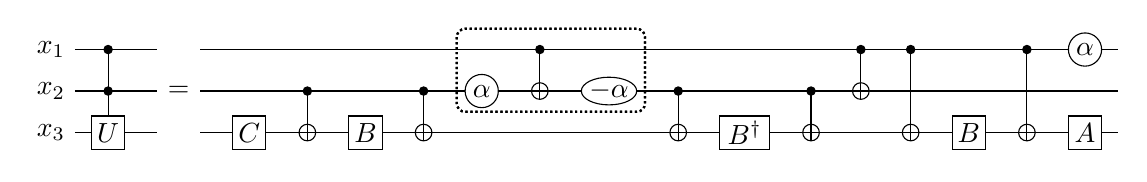
\begin{tikzpicture}[scale=1.000000,x=1pt,y=1pt]
\filldraw[color=white] (0.000000, -7.500000) rectangle (377.000000, 37.500000);
% Drawing wires
% Line 1: a3 W x_3
\draw[color=black] (0.000000,30.000000) -- (377.000000,30.000000);
\draw[color=black] (0.000000,30.000000) node[left] {$x_1$};
% Line 2: a2 W x_2
\draw[color=black] (0.000000,15.000000) -- (377.000000,15.000000);
\draw[color=black] (0.000000,15.000000) node[left] {$x_2$};
% Line 3: a1 W x_1
\draw[color=black] (0.000000,0.000000) -- (377.000000,0.000000);
\draw[color=black] (0.000000,0.000000) node[left] {$x_3$};
% Done with wires; drawing gates
% Line 4: a1 G $U$ a2 a3
\draw (12.000000,30.000000) -- (12.000000,0.000000);
\begin{scope}
\draw[fill=white] (12.000000, -0.000000) +(-45.000000:8.485281pt and 8.485281pt) -- +(45.000000:8.485281pt and 8.485281pt) -- +(135.000000:8.485281pt and 8.485281pt) -- +(225.000000:8.485281pt and 8.485281pt) -- cycle;
\clip (12.000000, -0.000000) +(-45.000000:8.485281pt and 8.485281pt) -- +(45.000000:8.485281pt and 8.485281pt) -- +(135.000000:8.485281pt and 8.485281pt) -- +(225.000000:8.485281pt and 8.485281pt) -- cycle;
\draw (12.000000, -0.000000) node {$U$};
\end{scope}
\filldraw (12.000000, 15.000000) circle(1.500000pt);
\filldraw (12.000000, 30.000000) circle(1.500000pt);
% Line 5: =
\draw[fill=white,color=white] (30.000000, -6.000000) rectangle (45.000000, 36.000000);
\draw (37.500000, 15.000000) node {$=$};
% Line 6: a1 G $C$
\begin{scope}
\draw[fill=white] (63.000000, -0.000000) +(-45.000000:8.485281pt and 8.485281pt) -- +(45.000000:8.485281pt and 8.485281pt) -- +(135.000000:8.485281pt and 8.485281pt) -- +(225.000000:8.485281pt and 8.485281pt) -- cycle;
\clip (63.000000, -0.000000) +(-45.000000:8.485281pt and 8.485281pt) -- +(45.000000:8.485281pt and 8.485281pt) -- +(135.000000:8.485281pt and 8.485281pt) -- +(225.000000:8.485281pt and 8.485281pt) -- cycle;
\draw (63.000000, -0.000000) node {$C$};
\end{scope}
% Line 7: +a1 a2
\draw (84.000000,15.000000) -- (84.000000,0.000000);
\begin{scope}
\draw[fill=white] (84.000000, 0.000000) circle(3.000000pt);
\clip (84.000000, 0.000000) circle(3.000000pt);
\draw (81.000000, 0.000000) -- (87.000000, 0.000000);
\draw (84.000000, -3.000000) -- (84.000000, 3.000000);
\end{scope}
\filldraw (84.000000, 15.000000) circle(1.500000pt);
% Line 8: a1 G $B$
\begin{scope}
\draw[fill=white] (105.000000, -0.000000) +(-45.000000:8.485281pt and 8.485281pt) -- +(45.000000:8.485281pt and 8.485281pt) -- +(135.000000:8.485281pt and 8.485281pt) -- +(225.000000:8.485281pt and 8.485281pt) -- cycle;
\clip (105.000000, -0.000000) +(-45.000000:8.485281pt and 8.485281pt) -- +(45.000000:8.485281pt and 8.485281pt) -- +(135.000000:8.485281pt and 8.485281pt) -- +(225.000000:8.485281pt and 8.485281pt) -- cycle;
\draw (105.000000, -0.000000) node {$B$};
\end{scope}
% Line 9: +a1 a2
\draw (126.000000,15.000000) -- (126.000000,0.000000);
\begin{scope}
\draw[fill=white] (126.000000, 0.000000) circle(3.000000pt);
\clip (126.000000, 0.000000) circle(3.000000pt);
\draw (123.000000, 0.000000) -- (129.000000, 0.000000);
\draw (126.000000, -3.000000) -- (126.000000, 3.000000);
\end{scope}
\filldraw (126.000000, 15.000000) circle(1.500000pt);
% Line 10: TOUCH
% Line 11: a2 P $\alpha$
\begin{scope}
\draw[fill=white] (147.000000, 15.000000) circle(6.000000pt);
\clip (147.000000, 15.000000) circle(6.000000pt);
\draw (147.000000, 15.000000) node {$\alpha$};
\end{scope}
% Line 12: +a2 a3
\draw (168.000000,30.000000) -- (168.000000,15.000000);
\begin{scope}
\draw[fill=white] (168.000000, 15.000000) circle(3.000000pt);
\clip (168.000000, 15.000000) circle(3.000000pt);
\draw (165.000000, 15.000000) -- (171.000000, 15.000000);
\draw (168.000000, 12.000000) -- (168.000000, 18.000000);
\end{scope}
\filldraw (168.000000, 30.000000) circle(1.500000pt);
% Line 13: a2 P $-\alpha$ height=10 width=20
\begin{scope}
\draw[fill=white] (193.000000, 15.000000) ellipse(10.000000pt and 5.000000pt);
\clip (193.000000, 15.000000) ellipse(10.000000pt and 5.000000pt);
\draw (193.000000, 15.000000) node {$-\alpha$};
\end{scope}
% Line 15: +a1 a2
\draw (218.000000,15.000000) -- (218.000000,0.000000);
\begin{scope}
\draw[fill=white] (218.000000, 0.000000) circle(3.000000pt);
\clip (218.000000, 0.000000) circle(3.000000pt);
\draw (215.000000, 0.000000) -- (221.000000, 0.000000);
\draw (218.000000, -3.000000) -- (218.000000, 3.000000);
\end{scope}
\filldraw (218.000000, 15.000000) circle(1.500000pt);
% Line 16: a1 G $B^\dagger$ width=18
\begin{scope}
\draw[fill=white] (242.000000, -0.000000) +(-45.000000:12.727922pt and 8.485281pt) -- +(45.000000:12.727922pt and 8.485281pt) -- +(135.000000:12.727922pt and 8.485281pt) -- +(225.000000:12.727922pt and 8.485281pt) -- cycle;
\clip (242.000000, -0.000000) +(-45.000000:12.727922pt and 8.485281pt) -- +(45.000000:12.727922pt and 8.485281pt) -- +(135.000000:12.727922pt and 8.485281pt) -- +(225.000000:12.727922pt and 8.485281pt) -- cycle;
\draw (242.000000, -0.000000) node {$B^\dagger$};
\end{scope}
% Line 17: +a1 a2
\draw (266.000000,15.000000) -- (266.000000,0.000000);
\begin{scope}
\draw[fill=white] (266.000000, 0.000000) circle(3.000000pt);
\clip (266.000000, 0.000000) circle(3.000000pt);
\draw (263.000000, 0.000000) -- (269.000000, 0.000000);
\draw (266.000000, -3.000000) -- (266.000000, 3.000000);
\end{scope}
\filldraw (266.000000, 15.000000) circle(1.500000pt);
% Line 18: +a2 a3
\draw (284.000000,30.000000) -- (284.000000,15.000000);
\begin{scope}
\draw[fill=white] (284.000000, 15.000000) circle(3.000000pt);
\clip (284.000000, 15.000000) circle(3.000000pt);
\draw (281.000000, 15.000000) -- (287.000000, 15.000000);
\draw (284.000000, 12.000000) -- (284.000000, 18.000000);
\end{scope}
\filldraw (284.000000, 30.000000) circle(1.500000pt);
% Line 19: +a1 a3
\draw (302.000000,30.000000) -- (302.000000,0.000000);
\begin{scope}
\draw[fill=white] (302.000000, 0.000000) circle(3.000000pt);
\clip (302.000000, 0.000000) circle(3.000000pt);
\draw (299.000000, 0.000000) -- (305.000000, 0.000000);
\draw (302.000000, -3.000000) -- (302.000000, 3.000000);
\end{scope}
\filldraw (302.000000, 30.000000) circle(1.500000pt);
% Line 20: a1 G $B$
\begin{scope}
\draw[fill=white] (323.000000, -0.000000) +(-45.000000:8.485281pt and 8.485281pt) -- +(45.000000:8.485281pt and 8.485281pt) -- +(135.000000:8.485281pt and 8.485281pt) -- +(225.000000:8.485281pt and 8.485281pt) -- cycle;
\clip (323.000000, -0.000000) +(-45.000000:8.485281pt and 8.485281pt) -- +(45.000000:8.485281pt and 8.485281pt) -- +(135.000000:8.485281pt and 8.485281pt) -- +(225.000000:8.485281pt and 8.485281pt) -- cycle;
\draw (323.000000, -0.000000) node {$B$};
\end{scope}
% Line 21: +a1 a3
\draw (344.000000,30.000000) -- (344.000000,0.000000);
\begin{scope}
\draw[fill=white] (344.000000, 0.000000) circle(3.000000pt);
\clip (344.000000, 0.000000) circle(3.000000pt);
\draw (341.000000, 0.000000) -- (347.000000, 0.000000);
\draw (344.000000, -3.000000) -- (344.000000, 3.000000);
\end{scope}
\filldraw (344.000000, 30.000000) circle(1.500000pt);
% Line 22: a1 G $A$
\begin{scope}
\draw[fill=white] (365.000000, -0.000000) +(-45.000000:8.485281pt and 8.485281pt) -- +(45.000000:8.485281pt and 8.485281pt) -- +(135.000000:8.485281pt and 8.485281pt) -- +(225.000000:8.485281pt and 8.485281pt) -- cycle;
\clip (365.000000, -0.000000) +(-45.000000:8.485281pt and 8.485281pt) -- +(45.000000:8.485281pt and 8.485281pt) -- +(135.000000:8.485281pt and 8.485281pt) -- +(225.000000:8.485281pt and 8.485281pt) -- cycle;
\draw (365.000000, -0.000000) node {$A$};
\end{scope}
% Line 23: a3 P $\alpha$
\begin{scope}
\draw[fill=white] (365.000000, 30.000000) circle(6.000000pt);
\clip (365.000000, 30.000000) circle(6.000000pt);
\draw (365.000000, 30.000000) node {$\alpha$};
\end{scope}
% Done with gates; drawing ending labels
% Done with ending labels; drawing cut lines and comments
% Line 14: a3 a2 @  3 color=black style=densely_dotted,thick,rounded_corners=3pt
\draw[draw opacity=1.000000,fill opacity=0.200000,color=black,densely dotted,thick,rounded corners=3pt] (138.000000,37.500000) rectangle (206.000000,7.500000);
\draw[draw opacity=1.000000,fill opacity=0.200000,color=black,densely dotted,thick,rounded corners=3pt] (138.000000,37.500000) rectangle (206.000000,7.500000);
% Done with comments
\end{tikzpicture}
\end{center}
\vspace{-10pt}
where we've drawn attention to the grouped $\alpha$, $-\alpha$, and \CNOT\ because we will investigate them as a group.  First the group must gain another \CNOT.  The \CNOT\ we'll gain is the 6th, but to gain it we need to temporarily introduce more \CNOT s.  Neither having been targeted by a \CNOT\ prior, the result of the third \CNOT\ is to calculate the ``parity'' of $\ket{x_1}$ and $\ket{x_2}$ in-place in $\ket{x_2}$ (phase of $\ket{x_2}$ ignored).  The 4th and 5th \CNOT s are then controlled by this parity. We can move the 6-th \CNOT\ to before the 4th, which will uncompute the parity (but not the phase), but we'll need to reconfigure \CNOT's 4 and 5 so that the result is once again a \NOT\ applied to $\ket{x_3}$ controlled by the \underline{parity} of $\ket{x_1}$ and $\ket{x_2}$, not just a \NOT\ controlled by $\ket{x_2}$.  To do this, note that applying \CNOT s to $\ket{x_3}$ controlled by $\ket{x_1}$, then another controlled by $\ket{x_2}$ results in a \NOT\ applied to $\ket{x_3}$ if and only if $\ket{x_1}\ket{x_2} = \ket{0}\ket{1}\mathrm{\ or\ }\ket{1}\ket{0}$, \textit{i.e.} a \CNOT\ controlled by the parity of $\ket{x_1}\ket{x_2}$.  So, we arrive at
\begin{center}
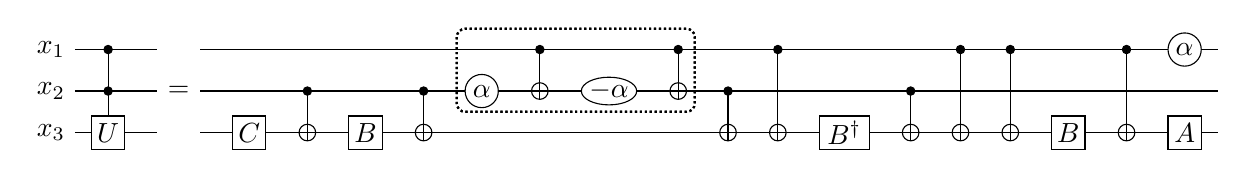
\begin{tikzpicture}[scale=1.000000,x=1pt,y=1pt]
\filldraw[color=white] (0.000000, -7.500000) rectangle (413.000000, 37.500000);
% Drawing wires
% Line 1: a3 W x_3
\draw[color=black] (0.000000,30.000000) -- (413.000000,30.000000);
\draw[color=black] (0.000000,30.000000) node[left] {$x_1$};
% Line 2: a2 W x_2
\draw[color=black] (0.000000,15.000000) -- (413.000000,15.000000);
\draw[color=black] (0.000000,15.000000) node[left] {$x_2$};
% Line 3: a1 W x_1
\draw[color=black] (0.000000,0.000000) -- (413.000000,0.000000);
\draw[color=black] (0.000000,0.000000) node[left] {$x_3$};
% Done with wires; drawing gates
% Line 4: a1 G $U$ a2 a3
\draw (12.000000,30.000000) -- (12.000000,0.000000);
\begin{scope}
\draw[fill=white] (12.000000, -0.000000) +(-45.000000:8.485281pt and 8.485281pt) -- +(45.000000:8.485281pt and 8.485281pt) -- +(135.000000:8.485281pt and 8.485281pt) -- +(225.000000:8.485281pt and 8.485281pt) -- cycle;
\clip (12.000000, -0.000000) +(-45.000000:8.485281pt and 8.485281pt) -- +(45.000000:8.485281pt and 8.485281pt) -- +(135.000000:8.485281pt and 8.485281pt) -- +(225.000000:8.485281pt and 8.485281pt) -- cycle;
\draw (12.000000, -0.000000) node {$U$};
\end{scope}
\filldraw (12.000000, 15.000000) circle(1.500000pt);
\filldraw (12.000000, 30.000000) circle(1.500000pt);
% Line 5: =
\draw[fill=white,color=white] (30.000000, -6.000000) rectangle (45.000000, 36.000000);
\draw (37.500000, 15.000000) node {$=$};
% Line 6: a1 G $C$
\begin{scope}
\draw[fill=white] (63.000000, -0.000000) +(-45.000000:8.485281pt and 8.485281pt) -- +(45.000000:8.485281pt and 8.485281pt) -- +(135.000000:8.485281pt and 8.485281pt) -- +(225.000000:8.485281pt and 8.485281pt) -- cycle;
\clip (63.000000, -0.000000) +(-45.000000:8.485281pt and 8.485281pt) -- +(45.000000:8.485281pt and 8.485281pt) -- +(135.000000:8.485281pt and 8.485281pt) -- +(225.000000:8.485281pt and 8.485281pt) -- cycle;
\draw (63.000000, -0.000000) node {$C$};
\end{scope}
% Line 7: +a1 a2
\draw (84.000000,15.000000) -- (84.000000,0.000000);
\begin{scope}
\draw[fill=white] (84.000000, 0.000000) circle(3.000000pt);
\clip (84.000000, 0.000000) circle(3.000000pt);
\draw (81.000000, 0.000000) -- (87.000000, 0.000000);
\draw (84.000000, -3.000000) -- (84.000000, 3.000000);
\end{scope}
\filldraw (84.000000, 15.000000) circle(1.500000pt);
% Line 8: a1 G $B$
\begin{scope}
\draw[fill=white] (105.000000, -0.000000) +(-45.000000:8.485281pt and 8.485281pt) -- +(45.000000:8.485281pt and 8.485281pt) -- +(135.000000:8.485281pt and 8.485281pt) -- +(225.000000:8.485281pt and 8.485281pt) -- cycle;
\clip (105.000000, -0.000000) +(-45.000000:8.485281pt and 8.485281pt) -- +(45.000000:8.485281pt and 8.485281pt) -- +(135.000000:8.485281pt and 8.485281pt) -- +(225.000000:8.485281pt and 8.485281pt) -- cycle;
\draw (105.000000, -0.000000) node {$B$};
\end{scope}
% Line 9: +a1 a2
\draw (126.000000,15.000000) -- (126.000000,0.000000);
\begin{scope}
\draw[fill=white] (126.000000, 0.000000) circle(3.000000pt);
\clip (126.000000, 0.000000) circle(3.000000pt);
\draw (123.000000, 0.000000) -- (129.000000, 0.000000);
\draw (126.000000, -3.000000) -- (126.000000, 3.000000);
\end{scope}
\filldraw (126.000000, 15.000000) circle(1.500000pt);
% Line 10: TOUCH
% Line 11: a2 P $\alpha$
\begin{scope}
\draw[fill=white] (147.000000, 15.000000) circle(6.000000pt);
\clip (147.000000, 15.000000) circle(6.000000pt);
\draw (147.000000, 15.000000) node {$\alpha$};
\end{scope}
% Line 12: +a2 a3
\draw (168.000000,30.000000) -- (168.000000,15.000000);
\begin{scope}
\draw[fill=white] (168.000000, 15.000000) circle(3.000000pt);
\clip (168.000000, 15.000000) circle(3.000000pt);
\draw (165.000000, 15.000000) -- (171.000000, 15.000000);
\draw (168.000000, 12.000000) -- (168.000000, 18.000000);
\end{scope}
\filldraw (168.000000, 30.000000) circle(1.500000pt);
% Line 13: a2 P $-\alpha$ height=10 width=20
\begin{scope}
\draw[fill=white] (193.000000, 15.000000) ellipse(10.000000pt and 5.000000pt);
\clip (193.000000, 15.000000) ellipse(10.000000pt and 5.000000pt);
\draw (193.000000, 15.000000) node {$-\alpha$};
\end{scope}
% Line 14: +a2 a3
\draw (218.000000,30.000000) -- (218.000000,15.000000);
\begin{scope}
\draw[fill=white] (218.000000, 15.000000) circle(3.000000pt);
\clip (218.000000, 15.000000) circle(3.000000pt);
\draw (215.000000, 15.000000) -- (221.000000, 15.000000);
\draw (218.000000, 12.000000) -- (218.000000, 18.000000);
\end{scope}
\filldraw (218.000000, 30.000000) circle(1.500000pt);
% Line 16: +a1 a2
\draw (236.000000,15.000000) -- (236.000000,0.000000);
\begin{scope}
\draw[fill=white] (236.000000, 0.000000) circle(3.000000pt);
\clip (236.000000, 0.000000) circle(3.000000pt);
\draw (233.000000, 0.000000) -- (239.000000, 0.000000);
\draw (236.000000, -3.000000) -- (236.000000, 3.000000);
\end{scope}
\filldraw (236.000000, 15.000000) circle(1.500000pt);
% Line 17: +a1 a3
\draw (254.000000,30.000000) -- (254.000000,0.000000);
\begin{scope}
\draw[fill=white] (254.000000, 0.000000) circle(3.000000pt);
\clip (254.000000, 0.000000) circle(3.000000pt);
\draw (251.000000, 0.000000) -- (257.000000, 0.000000);
\draw (254.000000, -3.000000) -- (254.000000, 3.000000);
\end{scope}
\filldraw (254.000000, 30.000000) circle(1.500000pt);
% Line 18: a1 G $B^\dagger$ width=18
\begin{scope}
\draw[fill=white] (278.000000, -0.000000) +(-45.000000:12.727922pt and 8.485281pt) -- +(45.000000:12.727922pt and 8.485281pt) -- +(135.000000:12.727922pt and 8.485281pt) -- +(225.000000:12.727922pt and 8.485281pt) -- cycle;
\clip (278.000000, -0.000000) +(-45.000000:12.727922pt and 8.485281pt) -- +(45.000000:12.727922pt and 8.485281pt) -- +(135.000000:12.727922pt and 8.485281pt) -- +(225.000000:12.727922pt and 8.485281pt) -- cycle;
\draw (278.000000, -0.000000) node {$B^\dagger$};
\end{scope}
% Line 19: +a1 a2
\draw (302.000000,15.000000) -- (302.000000,0.000000);
\begin{scope}
\draw[fill=white] (302.000000, 0.000000) circle(3.000000pt);
\clip (302.000000, 0.000000) circle(3.000000pt);
\draw (299.000000, 0.000000) -- (305.000000, 0.000000);
\draw (302.000000, -3.000000) -- (302.000000, 3.000000);
\end{scope}
\filldraw (302.000000, 15.000000) circle(1.500000pt);
% Line 20: +a1 a3
\draw (320.000000,30.000000) -- (320.000000,0.000000);
\begin{scope}
\draw[fill=white] (320.000000, 0.000000) circle(3.000000pt);
\clip (320.000000, 0.000000) circle(3.000000pt);
\draw (317.000000, 0.000000) -- (323.000000, 0.000000);
\draw (320.000000, -3.000000) -- (320.000000, 3.000000);
\end{scope}
\filldraw (320.000000, 30.000000) circle(1.500000pt);
% Line 21: +a1 a3
\draw (338.000000,30.000000) -- (338.000000,0.000000);
\begin{scope}
\draw[fill=white] (338.000000, 0.000000) circle(3.000000pt);
\clip (338.000000, 0.000000) circle(3.000000pt);
\draw (335.000000, 0.000000) -- (341.000000, 0.000000);
\draw (338.000000, -3.000000) -- (338.000000, 3.000000);
\end{scope}
\filldraw (338.000000, 30.000000) circle(1.500000pt);
% Line 22: a1 G $B$
\begin{scope}
\draw[fill=white] (359.000000, -0.000000) +(-45.000000:8.485281pt and 8.485281pt) -- +(45.000000:8.485281pt and 8.485281pt) -- +(135.000000:8.485281pt and 8.485281pt) -- +(225.000000:8.485281pt and 8.485281pt) -- cycle;
\clip (359.000000, -0.000000) +(-45.000000:8.485281pt and 8.485281pt) -- +(45.000000:8.485281pt and 8.485281pt) -- +(135.000000:8.485281pt and 8.485281pt) -- +(225.000000:8.485281pt and 8.485281pt) -- cycle;
\draw (359.000000, -0.000000) node {$B$};
\end{scope}
% Line 23: +a1 a3
\draw (380.000000,30.000000) -- (380.000000,0.000000);
\begin{scope}
\draw[fill=white] (380.000000, 0.000000) circle(3.000000pt);
\clip (380.000000, 0.000000) circle(3.000000pt);
\draw (377.000000, 0.000000) -- (383.000000, 0.000000);
\draw (380.000000, -3.000000) -- (380.000000, 3.000000);
\end{scope}
\filldraw (380.000000, 30.000000) circle(1.500000pt);
% Line 24: a1 G $A$
\begin{scope}
\draw[fill=white] (401.000000, -0.000000) +(-45.000000:8.485281pt and 8.485281pt) -- +(45.000000:8.485281pt and 8.485281pt) -- +(135.000000:8.485281pt and 8.485281pt) -- +(225.000000:8.485281pt and 8.485281pt) -- cycle;
\clip (401.000000, -0.000000) +(-45.000000:8.485281pt and 8.485281pt) -- +(45.000000:8.485281pt and 8.485281pt) -- +(135.000000:8.485281pt and 8.485281pt) -- +(225.000000:8.485281pt and 8.485281pt) -- cycle;
\draw (401.000000, -0.000000) node {$A$};
\end{scope}
% Line 25: a3 P $\alpha$
\begin{scope}
\draw[fill=white] (401.000000, 30.000000) circle(6.000000pt);
\clip (401.000000, 30.000000) circle(6.000000pt);
\draw (401.000000, 30.000000) node {$\alpha$};
\end{scope}
% Done with gates; drawing ending labels
% Done with ending labels; drawing cut lines and comments
% Line 15: a3 a2 @  4 color=black style=densely_dotted,thick,rounded_corners=3pt
\draw[draw opacity=1.000000,fill opacity=0.200000,color=black,densely dotted,thick,rounded corners=3pt] (138.000000,37.500000) rectangle (224.000000,7.500000);
\draw[draw opacity=1.000000,fill opacity=0.200000,color=black,densely dotted,thick,rounded corners=3pt] (138.000000,37.500000) rectangle (224.000000,7.500000);
% Done with comments
\end{tikzpicture}
\end{center}
\vspace{-10pt}
Now, the operation of the grouped gates on $\ket{x_1}\ket{x_2}$ can be expressed as
$$
\begin{bmatrix} 1 & 0 & 0 & 0 \\ 0 & 1 & 0 & 0 \\ 0 & 0 & 0 & 1 \\ 0 & 0 & 1 & 0 \end{bmatrix}
\begin{bmatrix} 1 & 0 & 0 & 0 \\ 0 & e^{-i\alpha} & 0 & 0 \\ 0 & 0 & 1 & 0 \\ 0 & 0& 0& e^{-i\alpha}\end{bmatrix}
\begin{bmatrix} 1 & 0 & 0 & 0 \\ 0 & 1 & 0 & 0 \\ 0 & 0 & 0 & 1 \\ 0 & 0 & 1 & 0 \end{bmatrix}
\begin{bmatrix} 1 & 0 & 0 & 0 \\ 0 & e^{i\alpha} & 0 & 0 \\ 0 & 0 & 1 & 0 \\ 0 & 0& 0& e^{i\alpha}\end{bmatrix}
=
\begin{bmatrix} 1 & 0 & 0 & 0 \\ 0 & 1 & 0 & 0 \\ 0 & 0 & e^{-i\alpha} & 0 \\ 0 & 0& 0& e^{i\alpha}\end{bmatrix}
$$
Being diagonal, the group can be transposed with any gate not targeting $\ket{x_1}$ or $\ket{x_2}$.  Doing so will only change when the relative phase corrections are performed in the circuit, not the final result.  We'll move it to the end to group the action only on $\ket{x_1}$ and $\ket{x_2}$. While we're at it, we'll move the final $\alpha$ to the start of the group, since it is diagonal and can be transposed with any gate not targeting $\ket{x_1}$.  Doing this allows the two \CNOT$(x_2,x_3)$s previously beside the group to cancel, along with the consecutive \CNOT$(x_1,x_3)$s between the $B^\dagger$ and $B$, giving the final circuit below with 8 single-qubit gates (including the $\alpha$'s and $-\alpha$) and 6 \CNOT s.
\begin{center}
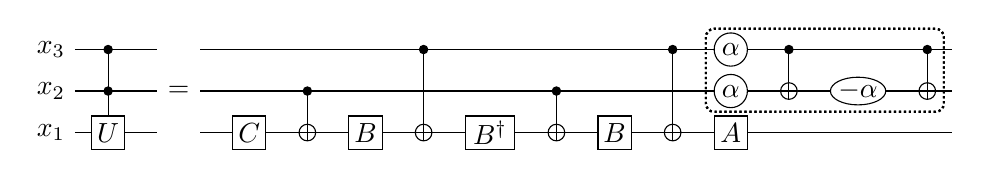
\begin{tikzpicture}[scale=1.000000,x=1pt,y=1pt]
\filldraw[color=white] (0.000000, -7.500000) rectangle (317.000000, 37.500000);
% Drawing wires
% Line 1: a3 W x_3
\draw[color=black] (0.000000,30.000000) -- (317.000000,30.000000);
\draw[color=black] (0.000000,30.000000) node[left] {$x_3$};
% Line 2: a2 W x_2
\draw[color=black] (0.000000,15.000000) -- (317.000000,15.000000);
\draw[color=black] (0.000000,15.000000) node[left] {$x_2$};
% Line 3: a1 W x_1
\draw[color=black] (0.000000,0.000000) -- (317.000000,0.000000);
\draw[color=black] (0.000000,0.000000) node[left] {$x_1$};
% Done with wires; drawing gates
% Line 4: a1 G $U$ a2 a3
\draw (12.000000,30.000000) -- (12.000000,0.000000);
\begin{scope}
\draw[fill=white] (12.000000, -0.000000) +(-45.000000:8.485281pt and 8.485281pt) -- +(45.000000:8.485281pt and 8.485281pt) -- +(135.000000:8.485281pt and 8.485281pt) -- +(225.000000:8.485281pt and 8.485281pt) -- cycle;
\clip (12.000000, -0.000000) +(-45.000000:8.485281pt and 8.485281pt) -- +(45.000000:8.485281pt and 8.485281pt) -- +(135.000000:8.485281pt and 8.485281pt) -- +(225.000000:8.485281pt and 8.485281pt) -- cycle;
\draw (12.000000, -0.000000) node {$U$};
\end{scope}
\filldraw (12.000000, 15.000000) circle(1.500000pt);
\filldraw (12.000000, 30.000000) circle(1.500000pt);
% Line 5: =
\draw[fill=white,color=white] (30.000000, -6.000000) rectangle (45.000000, 36.000000);
\draw (37.500000, 15.000000) node {$=$};
% Line 6: a1 G $C$
\begin{scope}
\draw[fill=white] (63.000000, -0.000000) +(-45.000000:8.485281pt and 8.485281pt) -- +(45.000000:8.485281pt and 8.485281pt) -- +(135.000000:8.485281pt and 8.485281pt) -- +(225.000000:8.485281pt and 8.485281pt) -- cycle;
\clip (63.000000, -0.000000) +(-45.000000:8.485281pt and 8.485281pt) -- +(45.000000:8.485281pt and 8.485281pt) -- +(135.000000:8.485281pt and 8.485281pt) -- +(225.000000:8.485281pt and 8.485281pt) -- cycle;
\draw (63.000000, -0.000000) node {$C$};
\end{scope}
% Line 7: +a1 a2
\draw (84.000000,15.000000) -- (84.000000,0.000000);
\begin{scope}
\draw[fill=white] (84.000000, 0.000000) circle(3.000000pt);
\clip (84.000000, 0.000000) circle(3.000000pt);
\draw (81.000000, 0.000000) -- (87.000000, 0.000000);
\draw (84.000000, -3.000000) -- (84.000000, 3.000000);
\end{scope}
\filldraw (84.000000, 15.000000) circle(1.500000pt);
% Line 8: a1 G $B$
\begin{scope}
\draw[fill=white] (105.000000, -0.000000) +(-45.000000:8.485281pt and 8.485281pt) -- +(45.000000:8.485281pt and 8.485281pt) -- +(135.000000:8.485281pt and 8.485281pt) -- +(225.000000:8.485281pt and 8.485281pt) -- cycle;
\clip (105.000000, -0.000000) +(-45.000000:8.485281pt and 8.485281pt) -- +(45.000000:8.485281pt and 8.485281pt) -- +(135.000000:8.485281pt and 8.485281pt) -- +(225.000000:8.485281pt and 8.485281pt) -- cycle;
\draw (105.000000, -0.000000) node {$B$};
\end{scope}
% Line 9: +a1 a3
\draw (126.000000,30.000000) -- (126.000000,0.000000);
\begin{scope}
\draw[fill=white] (126.000000, 0.000000) circle(3.000000pt);
\clip (126.000000, 0.000000) circle(3.000000pt);
\draw (123.000000, 0.000000) -- (129.000000, 0.000000);
\draw (126.000000, -3.000000) -- (126.000000, 3.000000);
\end{scope}
\filldraw (126.000000, 30.000000) circle(1.500000pt);
% Line 10: a1 G $B^\dagger$ width=18
\begin{scope}
\draw[fill=white] (150.000000, -0.000000) +(-45.000000:12.727922pt and 8.485281pt) -- +(45.000000:12.727922pt and 8.485281pt) -- +(135.000000:12.727922pt and 8.485281pt) -- +(225.000000:12.727922pt and 8.485281pt) -- cycle;
\clip (150.000000, -0.000000) +(-45.000000:12.727922pt and 8.485281pt) -- +(45.000000:12.727922pt and 8.485281pt) -- +(135.000000:12.727922pt and 8.485281pt) -- +(225.000000:12.727922pt and 8.485281pt) -- cycle;
\draw (150.000000, -0.000000) node {$B^\dagger$};
\end{scope}
% Line 11: +a1 a2
\draw (174.000000,15.000000) -- (174.000000,0.000000);
\begin{scope}
\draw[fill=white] (174.000000, 0.000000) circle(3.000000pt);
\clip (174.000000, 0.000000) circle(3.000000pt);
\draw (171.000000, 0.000000) -- (177.000000, 0.000000);
\draw (174.000000, -3.000000) -- (174.000000, 3.000000);
\end{scope}
\filldraw (174.000000, 15.000000) circle(1.500000pt);
% Line 12: a1 G $B$
\begin{scope}
\draw[fill=white] (195.000000, -0.000000) +(-45.000000:8.485281pt and 8.485281pt) -- +(45.000000:8.485281pt and 8.485281pt) -- +(135.000000:8.485281pt and 8.485281pt) -- +(225.000000:8.485281pt and 8.485281pt) -- cycle;
\clip (195.000000, -0.000000) +(-45.000000:8.485281pt and 8.485281pt) -- +(45.000000:8.485281pt and 8.485281pt) -- +(135.000000:8.485281pt and 8.485281pt) -- +(225.000000:8.485281pt and 8.485281pt) -- cycle;
\draw (195.000000, -0.000000) node {$B$};
\end{scope}
% Line 13: +a1 a3
\draw (216.000000,30.000000) -- (216.000000,0.000000);
\begin{scope}
\draw[fill=white] (216.000000, 0.000000) circle(3.000000pt);
\clip (216.000000, 0.000000) circle(3.000000pt);
\draw (213.000000, 0.000000) -- (219.000000, 0.000000);
\draw (216.000000, -3.000000) -- (216.000000, 3.000000);
\end{scope}
\filldraw (216.000000, 30.000000) circle(1.500000pt);
% Line 14: TOUCH
% Line 15: a1 G $A$
\begin{scope}
\draw[fill=white] (237.000000, -0.000000) +(-45.000000:8.485281pt and 8.485281pt) -- +(45.000000:8.485281pt and 8.485281pt) -- +(135.000000:8.485281pt and 8.485281pt) -- +(225.000000:8.485281pt and 8.485281pt) -- cycle;
\clip (237.000000, -0.000000) +(-45.000000:8.485281pt and 8.485281pt) -- +(45.000000:8.485281pt and 8.485281pt) -- +(135.000000:8.485281pt and 8.485281pt) -- +(225.000000:8.485281pt and 8.485281pt) -- cycle;
\draw (237.000000, -0.000000) node {$A$};
\end{scope}
% Line 16: a3 P $\alpha$
\begin{scope}
\draw[fill=white] (237.000000, 30.000000) circle(6.000000pt);
\clip (237.000000, 30.000000) circle(6.000000pt);
\draw (237.000000, 30.000000) node {$\alpha$};
\end{scope}
% Line 17: a2 P $\alpha$
\begin{scope}
\draw[fill=white] (237.000000, 15.000000) circle(6.000000pt);
\clip (237.000000, 15.000000) circle(6.000000pt);
\draw (237.000000, 15.000000) node {$\alpha$};
\end{scope}
% Line 18: +a2 a3
\draw (258.000000,30.000000) -- (258.000000,15.000000);
\begin{scope}
\draw[fill=white] (258.000000, 15.000000) circle(3.000000pt);
\clip (258.000000, 15.000000) circle(3.000000pt);
\draw (255.000000, 15.000000) -- (261.000000, 15.000000);
\draw (258.000000, 12.000000) -- (258.000000, 18.000000);
\end{scope}
\filldraw (258.000000, 30.000000) circle(1.500000pt);
% Line 19: a2 P $-\alpha$ height=10 width=20
\begin{scope}
\draw[fill=white] (283.000000, 15.000000) ellipse(10.000000pt and 5.000000pt);
\clip (283.000000, 15.000000) ellipse(10.000000pt and 5.000000pt);
\draw (283.000000, 15.000000) node {$-\alpha$};
\end{scope}
% Line 20: +a2 a3
\draw (308.000000,30.000000) -- (308.000000,15.000000);
\begin{scope}
\draw[fill=white] (308.000000, 15.000000) circle(3.000000pt);
\clip (308.000000, 15.000000) circle(3.000000pt);
\draw (305.000000, 15.000000) -- (311.000000, 15.000000);
\draw (308.000000, 12.000000) -- (308.000000, 18.000000);
\end{scope}
\filldraw (308.000000, 30.000000) circle(1.500000pt);
% Done with gates; drawing ending labels
% Done with ending labels; drawing cut lines and comments
% Line 21: a3 a2 @  4 color=black style=densely_dotted,thick,rounded_corners=3pt
\draw[draw opacity=1.000000,fill opacity=0.200000,color=black,densely dotted,thick,rounded corners=3pt] (228.000000,37.500000) rectangle (314.000000,7.500000);
\draw[draw opacity=1.000000,fill opacity=0.200000,color=black,densely dotted,thick,rounded corners=3pt] (228.000000,37.500000) rectangle (314.000000,7.500000);
% Done with comments
\end{tikzpicture}
\end{center}
\Textbf{4.23}
\Textbf{4.24} Verify that Figure 4.9 implements the Toffoli gate.
\begin{center}
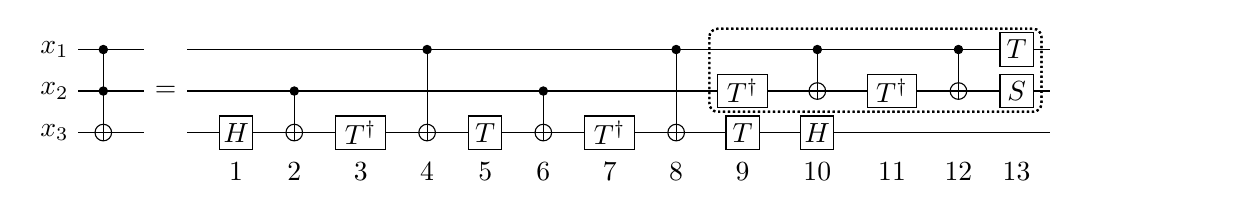
\begin{tikzpicture}[scale=1.000000,x=1pt,y=1pt]
\filldraw[color=white] (0.000000, -7.500000) rectangle (351.000000, 37.500000);
% Drawing wires
% Line 1: a3 W x_1
\draw[color=black] (0.000000,30.000000) -- (351.000000,30.000000);
\draw[color=black] (0.000000,30.000000) node[left] {$x_1$};
% Line 2: a2 W x_2
\draw[color=black] (0.000000,15.000000) -- (351.000000,15.000000);
\draw[color=black] (0.000000,15.000000) node[left] {$x_2$};
% Line 3: a1 W x_3
\draw[color=black] (0.000000,0.000000) -- (351.000000,0.000000);
\draw[color=black] (0.000000,0.000000) node[left] {$x_3$};
% Done with wires; drawing gates
% Line 4: +a1 a2 a3
\draw (9.000000,30.000000) -- (9.000000,0.000000);
\begin{scope}
\draw[fill=white] (9.000000, 0.000000) circle(3.000000pt);
\clip (9.000000, 0.000000) circle(3.000000pt);
\draw (6.000000, 0.000000) -- (12.000000, 0.000000);
\draw (9.000000, -3.000000) -- (9.000000, 3.000000);
\end{scope}
\filldraw (9.000000, 15.000000) circle(1.500000pt);
\filldraw (9.000000, 30.000000) circle(1.500000pt);
% Line 5: =
\draw[fill=white,color=white] (24.000000, -6.000000) rectangle (39.000000, 36.000000);
\draw (31.500000, 15.000000) node {$=$};
% Line 6: a1 H %% 1
\draw (57.000000, -7.500000) node[text width=144pt,below,text centered] {1};
\begin{scope}
\draw[fill=white] (57.000000, -0.000000) +(-45.000000:8.485281pt and 8.485281pt) -- +(45.000000:8.485281pt and 8.485281pt) -- +(135.000000:8.485281pt and 8.485281pt) -- +(225.000000:8.485281pt and 8.485281pt) -- cycle;
\clip (57.000000, -0.000000) +(-45.000000:8.485281pt and 8.485281pt) -- +(45.000000:8.485281pt and 8.485281pt) -- +(135.000000:8.485281pt and 8.485281pt) -- +(225.000000:8.485281pt and 8.485281pt) -- cycle;
\draw (57.000000, -0.000000) node {$H$};
\end{scope}
% Line 7: +a1 a2 %% 2
\draw (78.000000, -7.500000) node[text width=144pt,below,text centered] {2};
\draw (78.000000,15.000000) -- (78.000000,0.000000);
\begin{scope}
\draw[fill=white] (78.000000, 0.000000) circle(3.000000pt);
\clip (78.000000, 0.000000) circle(3.000000pt);
\draw (75.000000, 0.000000) -- (81.000000, 0.000000);
\draw (78.000000, -3.000000) -- (78.000000, 3.000000);
\end{scope}
\filldraw (78.000000, 15.000000) circle(1.500000pt);
% Line 8: a1 G $T^\dagger$ width=18 %% 3
\draw (102.000000, -7.500000) node[text width=144pt,below,text centered] {3};
\begin{scope}
\draw[fill=white] (102.000000, -0.000000) +(-45.000000:12.727922pt and 8.485281pt) -- +(45.000000:12.727922pt and 8.485281pt) -- +(135.000000:12.727922pt and 8.485281pt) -- +(225.000000:12.727922pt and 8.485281pt) -- cycle;
\clip (102.000000, -0.000000) +(-45.000000:12.727922pt and 8.485281pt) -- +(45.000000:12.727922pt and 8.485281pt) -- +(135.000000:12.727922pt and 8.485281pt) -- +(225.000000:12.727922pt and 8.485281pt) -- cycle;
\draw (102.000000, -0.000000) node {$T^\dagger$};
\end{scope}
% Line 9: +a1 a3 %% 4
\draw (126.000000, -7.500000) node[text width=144pt,below,text centered] {4};
\draw (126.000000,30.000000) -- (126.000000,0.000000);
\begin{scope}
\draw[fill=white] (126.000000, 0.000000) circle(3.000000pt);
\clip (126.000000, 0.000000) circle(3.000000pt);
\draw (123.000000, 0.000000) -- (129.000000, 0.000000);
\draw (126.000000, -3.000000) -- (126.000000, 3.000000);
\end{scope}
\filldraw (126.000000, 30.000000) circle(1.500000pt);
% Line 10: a1 G $T$ %% 5
\draw (147.000000, -7.500000) node[text width=144pt,below,text centered] {5};
\begin{scope}
\draw[fill=white] (147.000000, -0.000000) +(-45.000000:8.485281pt and 8.485281pt) -- +(45.000000:8.485281pt and 8.485281pt) -- +(135.000000:8.485281pt and 8.485281pt) -- +(225.000000:8.485281pt and 8.485281pt) -- cycle;
\clip (147.000000, -0.000000) +(-45.000000:8.485281pt and 8.485281pt) -- +(45.000000:8.485281pt and 8.485281pt) -- +(135.000000:8.485281pt and 8.485281pt) -- +(225.000000:8.485281pt and 8.485281pt) -- cycle;
\draw (147.000000, -0.000000) node {$T$};
\end{scope}
% Line 11: +a1 a2 %% 6
\draw (168.000000, -7.500000) node[text width=144pt,below,text centered] {6};
\draw (168.000000,15.000000) -- (168.000000,0.000000);
\begin{scope}
\draw[fill=white] (168.000000, 0.000000) circle(3.000000pt);
\clip (168.000000, 0.000000) circle(3.000000pt);
\draw (165.000000, 0.000000) -- (171.000000, 0.000000);
\draw (168.000000, -3.000000) -- (168.000000, 3.000000);
\end{scope}
\filldraw (168.000000, 15.000000) circle(1.500000pt);
% Line 12: a1 G $T^\dagger$ width=18 %% 7
\draw (192.000000, -7.500000) node[text width=144pt,below,text centered] {7};
\begin{scope}
\draw[fill=white] (192.000000, -0.000000) +(-45.000000:12.727922pt and 8.485281pt) -- +(45.000000:12.727922pt and 8.485281pt) -- +(135.000000:12.727922pt and 8.485281pt) -- +(225.000000:12.727922pt and 8.485281pt) -- cycle;
\clip (192.000000, -0.000000) +(-45.000000:12.727922pt and 8.485281pt) -- +(45.000000:12.727922pt and 8.485281pt) -- +(135.000000:12.727922pt and 8.485281pt) -- +(225.000000:12.727922pt and 8.485281pt) -- cycle;
\draw (192.000000, -0.000000) node {$T^\dagger$};
\end{scope}
% Line 13: +a1 a3 %% 8
\draw (216.000000, -7.500000) node[text width=144pt,below,text centered] {8};
\draw (216.000000,30.000000) -- (216.000000,0.000000);
\begin{scope}
\draw[fill=white] (216.000000, 0.000000) circle(3.000000pt);
\clip (216.000000, 0.000000) circle(3.000000pt);
\draw (213.000000, 0.000000) -- (219.000000, 0.000000);
\draw (216.000000, -3.000000) -- (216.000000, 3.000000);
\end{scope}
\filldraw (216.000000, 30.000000) circle(1.500000pt);
% Line 14: TOUCH
% Line 15: a2 G $T^\dagger$ width=18
\begin{scope}
\draw[fill=white] (240.000000, 15.000000) +(-45.000000:12.727922pt and 8.485281pt) -- +(45.000000:12.727922pt and 8.485281pt) -- +(135.000000:12.727922pt and 8.485281pt) -- +(225.000000:12.727922pt and 8.485281pt) -- cycle;
\clip (240.000000, 15.000000) +(-45.000000:12.727922pt and 8.485281pt) -- +(45.000000:12.727922pt and 8.485281pt) -- +(135.000000:12.727922pt and 8.485281pt) -- +(225.000000:12.727922pt and 8.485281pt) -- cycle;
\draw (240.000000, 15.000000) node {$T^\dagger$};
\end{scope}
% Line 16: a1 G $T$ %% 9
\draw (240.000000, -7.500000) node[text width=144pt,below,text centered] {9};
\begin{scope}
\draw[fill=white] (240.000000, -0.000000) +(-45.000000:8.485281pt and 8.485281pt) -- +(45.000000:8.485281pt and 8.485281pt) -- +(135.000000:8.485281pt and 8.485281pt) -- +(225.000000:8.485281pt and 8.485281pt) -- cycle;
\clip (240.000000, -0.000000) +(-45.000000:8.485281pt and 8.485281pt) -- +(45.000000:8.485281pt and 8.485281pt) -- +(135.000000:8.485281pt and 8.485281pt) -- +(225.000000:8.485281pt and 8.485281pt) -- cycle;
\draw (240.000000, -0.000000) node {$T$};
\end{scope}
% Line 17: a1 H
\begin{scope}
\draw[fill=white] (267.000000, -0.000000) +(-45.000000:8.485281pt and 8.485281pt) -- +(45.000000:8.485281pt and 8.485281pt) -- +(135.000000:8.485281pt and 8.485281pt) -- +(225.000000:8.485281pt and 8.485281pt) -- cycle;
\clip (267.000000, -0.000000) +(-45.000000:8.485281pt and 8.485281pt) -- +(45.000000:8.485281pt and 8.485281pt) -- +(135.000000:8.485281pt and 8.485281pt) -- +(225.000000:8.485281pt and 8.485281pt) -- cycle;
\draw (267.000000, -0.000000) node {$H$};
\end{scope}
% Line 18: +a2 a3 %% 10
\draw (267.000000, -7.500000) node[text width=144pt,below,text centered] {10};
\draw (267.000000,30.000000) -- (267.000000,15.000000);
\begin{scope}
\draw[fill=white] (267.000000, 15.000000) circle(3.000000pt);
\clip (267.000000, 15.000000) circle(3.000000pt);
\draw (264.000000, 15.000000) -- (270.000000, 15.000000);
\draw (267.000000, 12.000000) -- (267.000000, 18.000000);
\end{scope}
\filldraw (267.000000, 30.000000) circle(1.500000pt);
% Line 19: a2 G $T^\dagger$ width=18 %% 11
\draw (294.000000, -7.500000) node[text width=144pt,below,text centered] {11};
\begin{scope}
\draw[fill=white] (294.000000, 15.000000) +(-45.000000:12.727922pt and 8.485281pt) -- +(45.000000:12.727922pt and 8.485281pt) -- +(135.000000:12.727922pt and 8.485281pt) -- +(225.000000:12.727922pt and 8.485281pt) -- cycle;
\clip (294.000000, 15.000000) +(-45.000000:12.727922pt and 8.485281pt) -- +(45.000000:12.727922pt and 8.485281pt) -- +(135.000000:12.727922pt and 8.485281pt) -- +(225.000000:12.727922pt and 8.485281pt) -- cycle;
\draw (294.000000, 15.000000) node {$T^\dagger$};
\end{scope}
% Line 20: +a2 a3 %% 12
\draw (318.000000, -7.500000) node[text width=144pt,below,text centered] {12};
\draw (318.000000,30.000000) -- (318.000000,15.000000);
\begin{scope}
\draw[fill=white] (318.000000, 15.000000) circle(3.000000pt);
\clip (318.000000, 15.000000) circle(3.000000pt);
\draw (315.000000, 15.000000) -- (321.000000, 15.000000);
\draw (318.000000, 12.000000) -- (318.000000, 18.000000);
\end{scope}
\filldraw (318.000000, 30.000000) circle(1.500000pt);
% Line 21: a3 G $T$
\begin{scope}
\draw[fill=white] (339.000000, 30.000000) +(-45.000000:8.485281pt and 8.485281pt) -- +(45.000000:8.485281pt and 8.485281pt) -- +(135.000000:8.485281pt and 8.485281pt) -- +(225.000000:8.485281pt and 8.485281pt) -- cycle;
\clip (339.000000, 30.000000) +(-45.000000:8.485281pt and 8.485281pt) -- +(45.000000:8.485281pt and 8.485281pt) -- +(135.000000:8.485281pt and 8.485281pt) -- +(225.000000:8.485281pt and 8.485281pt) -- cycle;
\draw (339.000000, 30.000000) node {$T$};
\end{scope}
% Line 22: a2 G $S$ %% 13
\draw (339.000000, -7.500000) node[text width=144pt,below,text centered] {13};
\begin{scope}
\draw[fill=white] (339.000000, 15.000000) +(-45.000000:8.485281pt and 8.485281pt) -- +(45.000000:8.485281pt and 8.485281pt) -- +(135.000000:8.485281pt and 8.485281pt) -- +(225.000000:8.485281pt and 8.485281pt) -- cycle;
\clip (339.000000, 15.000000) +(-45.000000:8.485281pt and 8.485281pt) -- +(45.000000:8.485281pt and 8.485281pt) -- +(135.000000:8.485281pt and 8.485281pt) -- +(225.000000:8.485281pt and 8.485281pt) -- cycle;
\draw (339.000000, 15.000000) node {$S$};
\end{scope}
% Done with gates; drawing ending labels
% Done with ending labels; drawing cut lines and comments
% Line 23: a3 a2 @  5 color=black style=densely_dotted,thick,rounded_corners=3pt
\draw[draw opacity=1.000000,fill opacity=0.200000,color=black,densely dotted,thick,rounded corners=3pt] (228.000000,37.500000) rectangle (348.000000,7.500000);
\draw[draw opacity=1.000000,fill opacity=0.200000,color=black,densely dotted,thick,rounded corners=3pt] (228.000000,37.500000) rectangle (348.000000,7.500000);
% Done with comments
\end{tikzpicture}
\end{center}
\vspace{-15pt}
\Soln Define $V = \frac{1+i}{2}(I-iX), A=HT, B=T^\dagger, C=H$, and $\alpha=\pi/4$.  Note that this choice of $V$ is similar to that on page 182, but not exactly the same.  Still, we have $V^2=(\frac{1+i}{2})^2(I-iX)^2=\frac{i}{2}(I-2iX-X^2)=-i^2X=X$.  Also, $ABC=HTT^{\dagger}H = I$, and 
\begin{align*}
e^{i\alpha}AXBXC = \frac{1+i}{\sqrt{2}}HTXT^\dagger XH &=
\frac{1+i}{(\sqrt{2})^3}
\begin{bmatrix} 1 & 1 \\ 1 & -1 \end{bmatrix}
\begin{bmatrix} 1 & 0 \\  0 & e^{i\pi/4}\end{bmatrix}
\begin{bmatrix} 0 & 1 \\ 1 & 0 \end{bmatrix}
\begin{bmatrix} 1 & 0 \\  0 & e^{-i\pi/4}\end{bmatrix}
\begin{bmatrix} 0 & 1 \\ 1 & 0 \end{bmatrix}
\begin{bmatrix} 1 & 1 \\ 1 & -1 \end{bmatrix} \\
&= \frac{1+i}{2}\begin{bmatrix} 1 & -i \\ -i & 1 \end{bmatrix} = V 
\end{align*}
We conclude that the construction from Problem 4.22 applies.  With $\alpha=\pi/4$, note that 
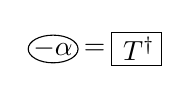
\begin{tikzpicture}[scale=1.000000,x=1pt,y=1pt]
\filldraw[color=white] (0.000000, -7.500000) rectangle (35.000000, 7.500000);
% Drawing wires
% Line 1: a W
%\draw[color=black] (0.000000,0.000000) -- (87.000000,0.000000);
% Done with wires; drawing gates
% Line 2: a P $-\alpha$ height=10 width=18
\begin{scope}
\draw[fill=white] (0.000000, 0.000000) ellipse(9.000000pt and 5.000000pt);
\clip (0.000000, 0.000000) ellipse(9.000000pt and 5.000000pt);
\draw (0.000000, 0.000000) node {$-\alpha$};
\end{scope}
% Line 3: =
%\draw[fill=white,color=white] (25.000000, -6.000000) rectangle (40.000000, 6.000000);
\draw (15.000000, 0.000000) node {$=$};
%% Line 4: a G $T^\dagger$ width=18
\begin{scope}
\draw[fill=white] (30.000000, -0.000000) +(-45.000000:12.727922pt and 8.485281pt) -- +(45.000000:12.727922pt and 8.485281pt) -- +(135.000000:12.727922pt and 8.485281pt) -- +(225.000000:12.727922pt and 8.485281pt) -- cycle;
\clip (30.000000, -0.000000) +(-45.000000:12.727922pt and 8.485281pt) -- +(45.000000:12.727922pt and 8.485281pt) -- +(135.000000:12.727922pt and 8.485281pt) -- +(225.000000:12.727922pt and 8.485281pt) -- cycle;
\draw (31.000000, -0.000000) node {$T^\dagger$};
\end{scope}
%% Done with gates; drawing ending labels
%% Done with ending labels; drawing cut lines and comments
%% Done with comments
\end{tikzpicture}
and
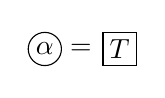
\begin{tikzpicture}[scale=1.000000,x=1pt,y=1pt]
\filldraw[color=white] (0.000000, -7.500000) rectangle (23.000000, 7.500000);
% Drawing wires
% Line 1: a W
%\draw[color=black] (0.000000,0.000000) -- (87.000000,0.000000);
% Done with wires; drawing gates
% Line 2: a P $-\alpha$ height=10 width=18
\begin{scope}
\draw[fill=white] (0.000000, 0.000000) circle(6.000000pt);
\clip (0.000000, 0.000000) circle(6.000000pt);
\draw (0.000000, 0.000000) node {$\alpha$};
\end{scope}
% Line 3: =
%\draw[fill=white,color=white] (25.000000, -6.000000) rectangle (40.000000, 6.000000);
\draw (13.000000, 0.000000) node {$=$};
%% Line 4: a G $T^\dagger$ width=18
\begin{scope}
\draw[fill=white] (27.000000, -0.000000) +(-45.000000:8.485281pt and 8.485281pt) -- +(45.000000:8.485281pt and 8.485281pt) -- +(135.000000:8.485281pt and 8.485281pt) -- +(225.000000:8.485281pt and 8.485281pt) -- cycle;
\clip (27.000000, -0.000000) +(-45.000000:8.485281pt and 8.485281pt) -- +(45.000000:8.485281pt and 8.485281pt) -- +(135.000000:8.485281pt and 8.485281pt) -- +(225.000000:8.485281pt and 8.485281pt) -- cycle;
\draw (27.000000, -0.000000) node {$T$};
\end{scope}
%% Done with gates; drawing ending labels
%% Done with ending labels; drawing cut lines and comments
%% Done with comments
\end{tikzpicture}.  So:
\begin{center}
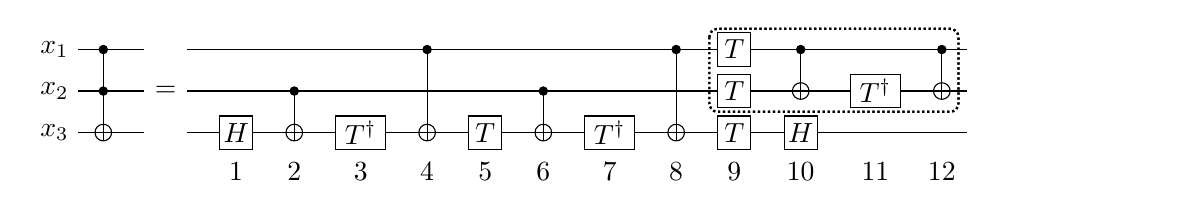
\begin{tikzpicture}[scale=1.000000,x=1pt,y=1pt]
\filldraw[color=white] (0.000000, -7.500000) rectangle (321.000000, 37.500000);
% Drawing wires
% Line 1: a3 W x_1
\draw[color=black] (0.000000,30.000000) -- (321.000000,30.000000);
\draw[color=black] (0.000000,30.000000) node[left] {$x_1$};
% Line 2: a2 W x_2
\draw[color=black] (0.000000,15.000000) -- (321.000000,15.000000);
\draw[color=black] (0.000000,15.000000) node[left] {$x_2$};
% Line 3: a1 W x_3
\draw[color=black] (0.000000,0.000000) -- (321.000000,0.000000);
\draw[color=black] (0.000000,0.000000) node[left] {$x_3$};
% Done with wires; drawing gates
% Line 4: +a1 a2 a3
\draw (9.000000,30.000000) -- (9.000000,0.000000);
\begin{scope}
\draw[fill=white] (9.000000, 0.000000) circle(3.000000pt);
\clip (9.000000, 0.000000) circle(3.000000pt);
\draw (6.000000, 0.000000) -- (12.000000, 0.000000);
\draw (9.000000, -3.000000) -- (9.000000, 3.000000);
\end{scope}
\filldraw (9.000000, 15.000000) circle(1.500000pt);
\filldraw (9.000000, 30.000000) circle(1.500000pt);
% Line 5: =
\draw[fill=white,color=white] (24.000000, -6.000000) rectangle (39.000000, 36.000000);
\draw (31.500000, 15.000000) node {$=$};
% Line 6: a1 H %% 1
\draw (57.000000, -7.500000) node[text width=144pt,below,text centered] {1};
\begin{scope}
\draw[fill=white] (57.000000, -0.000000) +(-45.000000:8.485281pt and 8.485281pt) -- +(45.000000:8.485281pt and 8.485281pt) -- +(135.000000:8.485281pt and 8.485281pt) -- +(225.000000:8.485281pt and 8.485281pt) -- cycle;
\clip (57.000000, -0.000000) +(-45.000000:8.485281pt and 8.485281pt) -- +(45.000000:8.485281pt and 8.485281pt) -- +(135.000000:8.485281pt and 8.485281pt) -- +(225.000000:8.485281pt and 8.485281pt) -- cycle;
\draw (57.000000, -0.000000) node {$H$};
\end{scope}
% Line 7: +a1 a2 %% 2
\draw (78.000000, -7.500000) node[text width=144pt,below,text centered] {2};
\draw (78.000000,15.000000) -- (78.000000,0.000000);
\begin{scope}
\draw[fill=white] (78.000000, 0.000000) circle(3.000000pt);
\clip (78.000000, 0.000000) circle(3.000000pt);
\draw (75.000000, 0.000000) -- (81.000000, 0.000000);
\draw (78.000000, -3.000000) -- (78.000000, 3.000000);
\end{scope}
\filldraw (78.000000, 15.000000) circle(1.500000pt);
% Line 8: a1 G $T^\dagger$ width=18 %% 3
\draw (102.000000, -7.500000) node[text width=144pt,below,text centered] {3};
\begin{scope}
\draw[fill=white] (102.000000, -0.000000) +(-45.000000:12.727922pt and 8.485281pt) -- +(45.000000:12.727922pt and 8.485281pt) -- +(135.000000:12.727922pt and 8.485281pt) -- +(225.000000:12.727922pt and 8.485281pt) -- cycle;
\clip (102.000000, -0.000000) +(-45.000000:12.727922pt and 8.485281pt) -- +(45.000000:12.727922pt and 8.485281pt) -- +(135.000000:12.727922pt and 8.485281pt) -- +(225.000000:12.727922pt and 8.485281pt) -- cycle;
\draw (102.000000, -0.000000) node {$T^\dagger$};
\end{scope}
% Line 9: +a1 a3 %% 4
\draw (126.000000, -7.500000) node[text width=144pt,below,text centered] {4};
\draw (126.000000,30.000000) -- (126.000000,0.000000);
\begin{scope}
\draw[fill=white] (126.000000, 0.000000) circle(3.000000pt);
\clip (126.000000, 0.000000) circle(3.000000pt);
\draw (123.000000, 0.000000) -- (129.000000, 0.000000);
\draw (126.000000, -3.000000) -- (126.000000, 3.000000);
\end{scope}
\filldraw (126.000000, 30.000000) circle(1.500000pt);
% Line 10: a1 G $T$ %% 5
\draw (147.000000, -7.500000) node[text width=144pt,below,text centered] {5};
\begin{scope}
\draw[fill=white] (147.000000, -0.000000) +(-45.000000:8.485281pt and 8.485281pt) -- +(45.000000:8.485281pt and 8.485281pt) -- +(135.000000:8.485281pt and 8.485281pt) -- +(225.000000:8.485281pt and 8.485281pt) -- cycle;
\clip (147.000000, -0.000000) +(-45.000000:8.485281pt and 8.485281pt) -- +(45.000000:8.485281pt and 8.485281pt) -- +(135.000000:8.485281pt and 8.485281pt) -- +(225.000000:8.485281pt and 8.485281pt) -- cycle;
\draw (147.000000, -0.000000) node {$T$};
\end{scope}
% Line 11: +a1 a2 %% 6
\draw (168.000000, -7.500000) node[text width=144pt,below,text centered] {6};
\draw (168.000000,15.000000) -- (168.000000,0.000000);
\begin{scope}
\draw[fill=white] (168.000000, 0.000000) circle(3.000000pt);
\clip (168.000000, 0.000000) circle(3.000000pt);
\draw (165.000000, 0.000000) -- (171.000000, 0.000000);
\draw (168.000000, -3.000000) -- (168.000000, 3.000000);
\end{scope}
\filldraw (168.000000, 15.000000) circle(1.500000pt);
% Line 12: a1 G $T^\dagger$ width=18 %% 7
\draw (192.000000, -7.500000) node[text width=144pt,below,text centered] {7};
\begin{scope}
\draw[fill=white] (192.000000, -0.000000) +(-45.000000:12.727922pt and 8.485281pt) -- +(45.000000:12.727922pt and 8.485281pt) -- +(135.000000:12.727922pt and 8.485281pt) -- +(225.000000:12.727922pt and 8.485281pt) -- cycle;
\clip (192.000000, -0.000000) +(-45.000000:12.727922pt and 8.485281pt) -- +(45.000000:12.727922pt and 8.485281pt) -- +(135.000000:12.727922pt and 8.485281pt) -- +(225.000000:12.727922pt and 8.485281pt) -- cycle;
\draw (192.000000, -0.000000) node {$T^\dagger$};
\end{scope}
% Line 13: +a1 a3 %% 8
\draw (216.000000, -7.500000) node[text width=144pt,below,text centered] {8};
\draw (216.000000,30.000000) -- (216.000000,0.000000);
\begin{scope}
\draw[fill=white] (216.000000, 0.000000) circle(3.000000pt);
\clip (216.000000, 0.000000) circle(3.000000pt);
\draw (213.000000, 0.000000) -- (219.000000, 0.000000);
\draw (216.000000, -3.000000) -- (216.000000, 3.000000);
\end{scope}
\filldraw (216.000000, 30.000000) circle(1.500000pt);
% Line 14: TOUCH
% Line 15: a3 G $T$
\begin{scope}
\draw[fill=white] (237.000000, 30.000000) +(-45.000000:8.485281pt and 8.485281pt) -- +(45.000000:8.485281pt and 8.485281pt) -- +(135.000000:8.485281pt and 8.485281pt) -- +(225.000000:8.485281pt and 8.485281pt) -- cycle;
\clip (237.000000, 30.000000) +(-45.000000:8.485281pt and 8.485281pt) -- +(45.000000:8.485281pt and 8.485281pt) -- +(135.000000:8.485281pt and 8.485281pt) -- +(225.000000:8.485281pt and 8.485281pt) -- cycle;
\draw (237.000000, 30.000000) node {$T$};
\end{scope}
% Line 16: a2 G $T$
\begin{scope}
\draw[fill=white] (237.000000, 15.000000) +(-45.000000:8.485281pt and 8.485281pt) -- +(45.000000:8.485281pt and 8.485281pt) -- +(135.000000:8.485281pt and 8.485281pt) -- +(225.000000:8.485281pt and 8.485281pt) -- cycle;
\clip (237.000000, 15.000000) +(-45.000000:8.485281pt and 8.485281pt) -- +(45.000000:8.485281pt and 8.485281pt) -- +(135.000000:8.485281pt and 8.485281pt) -- +(225.000000:8.485281pt and 8.485281pt) -- cycle;
\draw (237.000000, 15.000000) node {$T$};
\end{scope}
% Line 17: a1 G $T$ %% 9
\draw (237.000000, -7.500000) node[text width=144pt,below,text centered] {9};
\begin{scope}
\draw[fill=white] (237.000000, -0.000000) +(-45.000000:8.485281pt and 8.485281pt) -- +(45.000000:8.485281pt and 8.485281pt) -- +(135.000000:8.485281pt and 8.485281pt) -- +(225.000000:8.485281pt and 8.485281pt) -- cycle;
\clip (237.000000, -0.000000) +(-45.000000:8.485281pt and 8.485281pt) -- +(45.000000:8.485281pt and 8.485281pt) -- +(135.000000:8.485281pt and 8.485281pt) -- +(225.000000:8.485281pt and 8.485281pt) -- cycle;
\draw (237.000000, -0.000000) node {$T$};
\end{scope}
% Line 18: a1 H
\begin{scope}
\draw[fill=white] (261.000000, -0.000000) +(-45.000000:8.485281pt and 8.485281pt) -- +(45.000000:8.485281pt and 8.485281pt) -- +(135.000000:8.485281pt and 8.485281pt) -- +(225.000000:8.485281pt and 8.485281pt) -- cycle;
\clip (261.000000, -0.000000) +(-45.000000:8.485281pt and 8.485281pt) -- +(45.000000:8.485281pt and 8.485281pt) -- +(135.000000:8.485281pt and 8.485281pt) -- +(225.000000:8.485281pt and 8.485281pt) -- cycle;
\draw (261.000000, -0.000000) node {$H$};
\end{scope}
% Line 19: +a2 a3 %% 10
\draw (261.000000, -7.500000) node[text width=144pt,below,text centered] {10};
\draw (261.000000,30.000000) -- (261.000000,15.000000);
\begin{scope}
\draw[fill=white] (261.000000, 15.000000) circle(3.000000pt);
\clip (261.000000, 15.000000) circle(3.000000pt);
\draw (258.000000, 15.000000) -- (264.000000, 15.000000);
\draw (261.000000, 12.000000) -- (261.000000, 18.000000);
\end{scope}
\filldraw (261.000000, 30.000000) circle(1.500000pt);
% Line 20: a2 G $T^\dagger$ width=18 %% 11
\draw (288.000000, -7.500000) node[text width=144pt,below,text centered] {11};
\begin{scope}
\draw[fill=white] (288.000000, 15.000000) +(-45.000000:12.727922pt and 8.485281pt) -- +(45.000000:12.727922pt and 8.485281pt) -- +(135.000000:12.727922pt and 8.485281pt) -- +(225.000000:12.727922pt and 8.485281pt) -- cycle;
\clip (288.000000, 15.000000) +(-45.000000:12.727922pt and 8.485281pt) -- +(45.000000:12.727922pt and 8.485281pt) -- +(135.000000:12.727922pt and 8.485281pt) -- +(225.000000:12.727922pt and 8.485281pt) -- cycle;
\draw (288.000000, 15.000000) node {$T^\dagger$};
\end{scope}
% Line 21: +a2 a3 %% 12
\draw (312.000000, -7.500000) node[text width=144pt,below,text centered] {12};
\draw (312.000000,30.000000) -- (312.000000,15.000000);
\begin{scope}
\draw[fill=white] (312.000000, 15.000000) circle(3.000000pt);
\clip (312.000000, 15.000000) circle(3.000000pt);
\draw (309.000000, 15.000000) -- (315.000000, 15.000000);
\draw (312.000000, 12.000000) -- (312.000000, 18.000000);
\end{scope}
\filldraw (312.000000, 30.000000) circle(1.500000pt);
% Done with gates; drawing ending labels
% Done with ending labels; drawing cut lines and comments
% Line 22: a3 a2 @  4 color=black style=densely_dotted,thick,rounded_corners=3pt
\draw[draw opacity=1.000000,fill opacity=0.200000,color=black,densely dotted,thick,rounded corners=3pt] (228.000000,37.500000) rectangle (318.000000,7.500000);
\draw[draw opacity=1.000000,fill opacity=0.200000,color=black,densely dotted,thick,rounded corners=3pt] (228.000000,37.500000) rectangle (318.000000,7.500000);
% Done with comments
\end{tikzpicture}
\end{center}
\vspace{-10pt}
All that remains is to show that the grouped subcircuits are equivalent, that is, to show that
\begin{center}
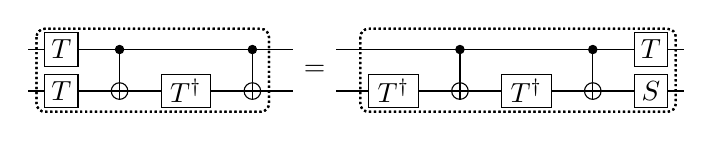
\begin{tikzpicture}[scale=1.000000,x=1pt,y=1pt]
\filldraw[color=white] (0.000000, -7.500000) rectangle (237.000000, 22.500000);
% Drawing wires
% Line 1: a2 W
\draw[color=black] (0.000000,15.000000) -- (237.000000,15.000000);
% Line 2: a1 W
\draw[color=black] (0.000000,0.000000) -- (237.000000,0.000000);
% Done with wires; drawing gates
% Line 3: a2 G $T$
\begin{scope}
\draw[fill=white] (12.000000, 15.000000) +(-45.000000:8.485281pt and 8.485281pt) -- +(45.000000:8.485281pt and 8.485281pt) -- +(135.000000:8.485281pt and 8.485281pt) -- +(225.000000:8.485281pt and 8.485281pt) -- cycle;
\clip (12.000000, 15.000000) +(-45.000000:8.485281pt and 8.485281pt) -- +(45.000000:8.485281pt and 8.485281pt) -- +(135.000000:8.485281pt and 8.485281pt) -- +(225.000000:8.485281pt and 8.485281pt) -- cycle;
\draw (12.000000, 15.000000) node {$T$};
\end{scope}
% Line 4: a1 G $T$
\begin{scope}
\draw[fill=white] (12.000000, -0.000000) +(-45.000000:8.485281pt and 8.485281pt) -- +(45.000000:8.485281pt and 8.485281pt) -- +(135.000000:8.485281pt and 8.485281pt) -- +(225.000000:8.485281pt and 8.485281pt) -- cycle;
\clip (12.000000, -0.000000) +(-45.000000:8.485281pt and 8.485281pt) -- +(45.000000:8.485281pt and 8.485281pt) -- +(135.000000:8.485281pt and 8.485281pt) -- +(225.000000:8.485281pt and 8.485281pt) -- cycle;
\draw (12.000000, -0.000000) node {$T$};
\end{scope}
% Line 5: +a1 a2
\draw (33.000000,15.000000) -- (33.000000,0.000000);
\begin{scope}
\draw[fill=white] (33.000000, 0.000000) circle(3.000000pt);
\clip (33.000000, 0.000000) circle(3.000000pt);
\draw (30.000000, 0.000000) -- (36.000000, 0.000000);
\draw (33.000000, -3.000000) -- (33.000000, 3.000000);
\end{scope}
\filldraw (33.000000, 15.000000) circle(1.500000pt);
% Line 6: a1 G $T^\dagger$ width=18
\begin{scope}
\draw[fill=white] (57.000000, -0.000000) +(-45.000000:12.727922pt and 8.485281pt) -- +(45.000000:12.727922pt and 8.485281pt) -- +(135.000000:12.727922pt and 8.485281pt) -- +(225.000000:12.727922pt and 8.485281pt) -- cycle;
\clip (57.000000, -0.000000) +(-45.000000:12.727922pt and 8.485281pt) -- +(45.000000:12.727922pt and 8.485281pt) -- +(135.000000:12.727922pt and 8.485281pt) -- +(225.000000:12.727922pt and 8.485281pt) -- cycle;
\draw (57.000000, -0.000000) node {$T^\dagger$};
\end{scope}
% Line 7: +a1 a2
\draw (81.000000,15.000000) -- (81.000000,0.000000);
\begin{scope}
\draw[fill=white] (81.000000, 0.000000) circle(3.000000pt);
\clip (81.000000, 0.000000) circle(3.000000pt);
\draw (78.000000, 0.000000) -- (84.000000, 0.000000);
\draw (81.000000, -3.000000) -- (81.000000, 3.000000);
\end{scope}
\filldraw (81.000000, 15.000000) circle(1.500000pt);
% Line 9: =
\draw[fill=white,color=white] (96.000000, -6.000000) rectangle (111.000000, 21.000000);
\draw (103.500000, 7.500000) node {$=$};
% Line 10: a1 G $T^\dagger$ width=18
\begin{scope}
\draw[fill=white] (132.000000, -0.000000) +(-45.000000:12.727922pt and 8.485281pt) -- +(45.000000:12.727922pt and 8.485281pt) -- +(135.000000:12.727922pt and 8.485281pt) -- +(225.000000:12.727922pt and 8.485281pt) -- cycle;
\clip (132.000000, -0.000000) +(-45.000000:12.727922pt and 8.485281pt) -- +(45.000000:12.727922pt and 8.485281pt) -- +(135.000000:12.727922pt and 8.485281pt) -- +(225.000000:12.727922pt and 8.485281pt) -- cycle;
\draw (132.000000, -0.000000) node {$T^\dagger$};
\end{scope}
% Line 11: +a1 a2
\draw (156.000000,15.000000) -- (156.000000,0.000000);
\begin{scope}
\draw[fill=white] (156.000000, 0.000000) circle(3.000000pt);
\clip (156.000000, 0.000000) circle(3.000000pt);
\draw (153.000000, 0.000000) -- (159.000000, 0.000000);
\draw (156.000000, -3.000000) -- (156.000000, 3.000000);
\end{scope}
\filldraw (156.000000, 15.000000) circle(1.500000pt);
% Line 12: a1 G $T^\dagger$ width=18
\begin{scope}
\draw[fill=white] (180.000000, -0.000000) +(-45.000000:12.727922pt and 8.485281pt) -- +(45.000000:12.727922pt and 8.485281pt) -- +(135.000000:12.727922pt and 8.485281pt) -- +(225.000000:12.727922pt and 8.485281pt) -- cycle;
\clip (180.000000, -0.000000) +(-45.000000:12.727922pt and 8.485281pt) -- +(45.000000:12.727922pt and 8.485281pt) -- +(135.000000:12.727922pt and 8.485281pt) -- +(225.000000:12.727922pt and 8.485281pt) -- cycle;
\draw (180.000000, -0.000000) node {$T^\dagger$};
\end{scope}
% Line 13: +a1 a2
\draw (204.000000,15.000000) -- (204.000000,0.000000);
\begin{scope}
\draw[fill=white] (204.000000, 0.000000) circle(3.000000pt);
\clip (204.000000, 0.000000) circle(3.000000pt);
\draw (201.000000, 0.000000) -- (207.000000, 0.000000);
\draw (204.000000, -3.000000) -- (204.000000, 3.000000);
\end{scope}
\filldraw (204.000000, 15.000000) circle(1.500000pt);
% Line 14: a2 G $T$
\begin{scope}
\draw[fill=white] (225.000000, 15.000000) +(-45.000000:8.485281pt and 8.485281pt) -- +(45.000000:8.485281pt and 8.485281pt) -- +(135.000000:8.485281pt and 8.485281pt) -- +(225.000000:8.485281pt and 8.485281pt) -- cycle;
\clip (225.000000, 15.000000) +(-45.000000:8.485281pt and 8.485281pt) -- +(45.000000:8.485281pt and 8.485281pt) -- +(135.000000:8.485281pt and 8.485281pt) -- +(225.000000:8.485281pt and 8.485281pt) -- cycle;
\draw (225.000000, 15.000000) node {$T$};
\end{scope}
% Line 15: a1 G $S$
\begin{scope}
\draw[fill=white] (225.000000, -0.000000) +(-45.000000:8.485281pt and 8.485281pt) -- +(45.000000:8.485281pt and 8.485281pt) -- +(135.000000:8.485281pt and 8.485281pt) -- +(225.000000:8.485281pt and 8.485281pt) -- cycle;
\clip (225.000000, -0.000000) +(-45.000000:8.485281pt and 8.485281pt) -- +(45.000000:8.485281pt and 8.485281pt) -- +(135.000000:8.485281pt and 8.485281pt) -- +(225.000000:8.485281pt and 8.485281pt) -- cycle;
\draw (225.000000, -0.000000) node {$S$};
\end{scope}
% Done with gates; drawing ending labels
% Done with ending labels; drawing cut lines and comments
% Line 8: a2 a1 @  4 color=black style=densely_dotted,thick,rounded_corners=3pt
\draw[draw opacity=1.000000,fill opacity=0.200000,color=black,densely dotted,thick,rounded corners=3pt] (3.000000,22.500000) rectangle (87.000000,-7.500000);
\draw[draw opacity=1.000000,fill opacity=0.200000,color=black,densely dotted,thick,rounded corners=3pt] (3.000000,22.500000) rectangle (87.000000,-7.500000);
% Line 16: a2 a1 @  5 color=black style=densely_dotted,thick,rounded_corners=3pt
\draw[draw opacity=1.000000,fill opacity=0.200000,color=black,densely dotted,thick,rounded corners=3pt] (120.000000,22.500000) rectangle (234.000000,-7.500000);
\draw[draw opacity=1.000000,fill opacity=0.200000,color=black,densely dotted,thick,rounded corners=3pt] (120.000000,22.500000) rectangle (234.000000,-7.500000);
% Done with comments
\end{tikzpicture}
\end{center}
\vspace{-10pt}
We do this by matrix mutiplication.  On the left, we have:
$$\begin{bmatrix} 1 & 0 & 0 &0 \\ 0 & 1 & 0 & 0 \\ 0 & 0 & 0 & 1 \\ 0 & 0 & 1 & 0\end{bmatrix}
\begin{bmatrix} 1 & 0 & 0 &0 \\ 0 & e^{-i\pi/4} & 0 & 0 \\ 0 & 0 & 1 & 0 \\ 0 & 0 & 0 & e^{-i\pi/4}\end{bmatrix}
\begin{bmatrix} 1 & 0 & 0 &0 \\ 0 & 1 & 0 & 0 \\ 0 & 0 & 0 & 1 \\ 0 & 0 & 1 & 0\end{bmatrix}
\begin{bmatrix} 1 & 0 & 0 &0 \\ 0 & 1 & 0 & 0 \\ 0 & 0 & e^{i\pi/4} & 0 \\ 0 & 0 & 0 & e^{i\pi/4}\end{bmatrix}
\begin{bmatrix} 1 & 0 & 0 &0 \\ 0 & e^{i\pi/4} & 0 & 0 \\ 0 & 0 & 1 & 0 \\ 0 & 0 & 0 & e^{i\pi/4}\end{bmatrix}$$
$$ = \begin{bmatrix} 1 & 0 & 0 &0 \\ 0 & 1 & 0 & 0 \\ 0 & 0 & 1 & 0 \\ 0 & 0 & 0 & i\end{bmatrix}$$
On the right:
$$
\begin{bmatrix} 1 & 0 & 0 &0 \\ 0 & i & 0 & 0 \\ 0 & 0 & 1 & 0 \\ 0 & 0 & 0 & i\end{bmatrix}
\begin{bmatrix} 1 & 0 & 0 &0 \\ 0 & 1 & 0 & 0 \\ 0 & 0 & e^{i\pi/4} & 0 \\ 0 & 0 & 0 & e^{i\pi/4}\end{bmatrix}
\begin{bmatrix} 1 & 0 & 0 &0 \\ 0 & 1 & 0 & 0 \\ 0 & 0 & 0 & 1 \\ 0 & 0 & 1 & 0\end{bmatrix}
\begin{bmatrix} 1 & 0 & 0 &0 \\ 0 & e^{-i\pi/4} & 0 & 0 \\ 0 & 0 & 1 & 0 \\ 0 & 0 & 0 & e^{-i\pi/4}\end{bmatrix}
\begin{bmatrix} 1 & 0 & 0 &0 \\ 0 & 1 & 0 & 0 \\ 0 & 0 & 0 & 1 \\ 0 & 0 & 1 & 0\end{bmatrix}\ \ \ \ \setminus$$
$$\cdot\begin{bmatrix} 1 & 0 & 0 &0 \\ 0 & e^{-i\pi/4} & 0 & 0 \\ 0 & 0 & 1 & 0 \\ 0 & 0 & 0 & e^{-i\pi/4}\end{bmatrix} = \begin{bmatrix} 1 & 0 & 0 &0 \\ 0 & 1 & 0 & 0 \\ 0 & 0 & 1 & 0 \\ 0 & 0 & 0 & i\end{bmatrix}$$
So, the subcircuits are equivalent and Figure 4.9 implements the Toffoli gate.  Note that both subcircuits execute a controlled-$S$ gate on $\ket{x_2}$, controlled by $\ket{x_1}$,  The subcircuit in the construction provided by the exercise is the result of a direct application of Figure 6, where $A=S, B=C=T^\dagger$, and $\alpha =\pi/4$, since $ABC=S(T^\dagger)^2=SS^\dagger=I$, and $e^{i\alpha}AXBXC=e^{i\pi/4}SXT^\dagger XT^\dagger= S$ can be easily verified via matrix-multiplication

\Textbf{4.25} Recall that the Fredkin (controlled-swap) gate performs the transform
$$\begin{bmatrix}
1 & 0 & 0 & 0 & 0 & 0 & 0 & 0 \\
0 & 1 & 0 & 0 & 0 & 0 & 0 & 0 \\
0 & 0 & 1 & 0 & 0 & 0 & 0 & 0 \\
0 & 0 & 0 & 1 & 0 & 0 & 0 & 0 \\
0 & 0 & 0 & 0 & 1 & 0 & 0 & 0 \\
0 & 0 & 0 & 0 & 0 & 0 & 1 & 0 \\
0 & 0 & 0 & 0 & 0 & 1 & 0 & 0 \\
0 & 0 & 0 & 0 & 0 & 0 & 0 & 1 
\end{bmatrix}$$
\begin{enumerate}
\item Give a quantum circuit which uses three Toffoli gates to construct the Fredkin gate (\textit{Hint:} think of the swap gate construction - you can control each gate one at a time)
\item Show that the first and last Toffoli gates can be replaced by \CNOT\ gates.
\item Now replace the middle Toffoli gate with the circuit in Figure 4.8 to obtain a Fredkin gate construction using only six two-qubit gates
\item Can you come up with an even simpler construction, with only five two-qubit gates?
\end{enumerate}
\vspace{-15pt}
\Soln For part 1, we'll show the following circuit identity by tracing the result of each computational basis state through each of the three Toffolis, indexed 1-3.
\begin{center}\ \ \ \ \ \ \ \ \ \ \ \ \ \ 
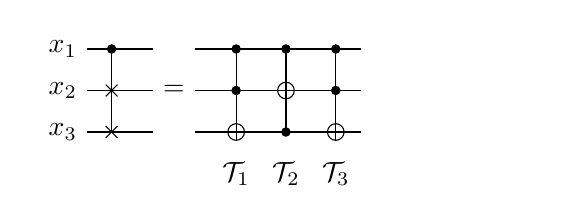
\begin{tikzpicture}[scale=1.000000,x=1pt,y=1pt]
\filldraw[color=white] (0.000000, -7.500000) rectangle (99.000000, 37.500000);
% Drawing wires
% Line 1: a3 W x_3
\draw[color=black] (0.000000,30.000000) -- (99.000000,30.000000);
\draw[color=black] (0.000000,30.000000) node[left] {$x_1$};
% Line 2: a2 W x_2
\draw[color=black] (0.000000,15.000000) -- (99.000000,15.000000);
\draw[color=black] (0.000000,15.000000) node[left] {$x_2$};
% Line 3: a1 W x_1
\draw[color=black] (0.000000,0.000000) -- (99.000000,0.000000);
\draw[color=black] (0.000000,0.000000) node[left] {$x_3$};
% Done with wires; drawing gates
% Line 4: a1 a2 SWAP a3
\draw (9.000000,30.000000) -- (9.000000,0.000000);
\begin{scope}
\draw (6.878680, -2.121320) -- (11.121320, 2.121320);
\draw (6.878680, 2.121320) -- (11.121320, -2.121320);
\end{scope}
\begin{scope}
\draw (6.878680, 12.878680) -- (11.121320, 17.121320);
\draw (6.878680, 17.121320) -- (11.121320, 12.878680);
\end{scope}
\filldraw (9.000000, 30.000000) circle(1.500000pt);
% Line 5: =
\draw[fill=white,color=white] (24.000000, -6.000000) rectangle (39.000000, 36.000000);
\draw (31.500000, 15.000000) node {$=$};
% Line 6: a1 T a2 a3 %% $\mathcal{T}_1$
\draw (54.000000, -7.500000) node[text width=144pt,below,text centered] {$\mathcal{T}_1$};
\draw (54.000000,30.000000) -- (54.000000,0.000000);
\begin{scope}
\draw[fill=white] (54.000000, 0.000000) circle(3.000000pt);
\clip (54.000000, 0.000000) circle(3.000000pt);
\draw (51.000000, 0.000000) -- (57.000000, 0.000000);
\draw (54.000000, -3.000000) -- (54.000000, 3.000000);
\end{scope}
\filldraw (54.000000, 15.000000) circle(1.500000pt);
\filldraw (54.000000, 30.000000) circle(1.500000pt);
% Line 7: a2 T a1 a3 %% $\mathcal{T}_2$
\draw (72.000000, -7.500000) node[text width=144pt,below,text centered] {$\mathcal{T}_2$};
\draw (72.000000,30.000000) -- (72.000000,0.000000);
\begin{scope}
\draw[fill=white] (72.000000, 15.000000) circle(3.000000pt);
\clip (72.000000, 15.000000) circle(3.000000pt);
\draw (69.000000, 15.000000) -- (75.000000, 15.000000);
\draw (72.000000, 12.000000) -- (72.000000, 18.000000);
\end{scope}
\filldraw (72.000000, 0.000000) circle(1.500000pt);
\filldraw (72.000000, 30.000000) circle(1.500000pt);
% Line 8: a1 T a2 a3 %% $\mathcal{T}_3$
\draw (90.000000, -7.500000) node[text width=144pt,below,text centered] {$\mathcal{T}_3$};
\draw (90.000000,30.000000) -- (90.000000,0.000000);
\begin{scope}
\draw[fill=white] (90.000000, 0.000000) circle(3.000000pt);
\clip (90.000000, 0.000000) circle(3.000000pt);
\draw (87.000000, 0.000000) -- (93.000000, 0.000000);
\draw (90.000000, -3.000000) -- (90.000000, 3.000000);
\end{scope}
\filldraw (90.000000, 15.000000) circle(1.500000pt);
\filldraw (90.000000, 30.000000) circle(1.500000pt);
% Done with gates; drawing ending labels
% Done with ending labels; drawing cut lines and comments
% Done with comments
\end{tikzpicture}
\end{center}
\vspace{-10pt}
\begin{center}
\begin{tabular}{c|c|c|c|} 
$\ket{x_1x_2x_3}$ & $\mathcal{T}_1$ & $\mathcal{T}_2$ & $\mathcal{T}_3$ \\
\hline
$\ket{000}$ & $\ket{000}$ & $\ket{000}$ & $\ket{000}$  \\
\hline
$\ket{001}$  & $\ket{001}$ & $\ket{001}$ & $\ket{001}$ \\
\hline
$\ket{010}$ & $\ket{010}$ & $\ket{010}$ & $\ket{010}$ \\
\hline
$\ket{011}$& $\ket{011}$ & $\ket{011}$ & $\ket{011}$ \\
\hline
$\ket{100}$ & $\ket{100}$ & $\ket{100}$ & $\ket{100}$ \\
\hline
$\ket{101}$ & $\ket{101}$ & $\ket{111}$ & $\ket{110}$ \\
\hline
$\ket{110}$ & $\ket{111}$ & $\ket{101}$ & $\ket{101}$ \\
\hline
$\ket{111}$ & $\ket{110}$ & $\ket{110}$ & $\ket{111}$ 
\end{tabular}
\end{center}
\vspace{-10pt}
For part 2, we replace $\mathcal{T}_1$ and $\mathcal{T}_3$ with \CNOT$(x_2, x_3)$.
\begin{center}\ \ \ \ \ \ \ \ \ \ \ \ \ \ 
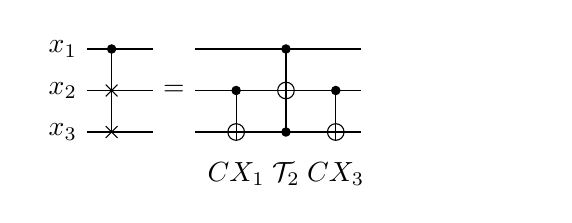
\begin{tikzpicture}[scale=1.000000,x=1pt,y=1pt]
\filldraw[color=white] (0.000000, -7.500000) rectangle (99.000000, 37.500000);
% Drawing wires
% Line 1: a3 W x_1
\draw[color=black] (0.000000,30.000000) -- (99.000000,30.000000);
\draw[color=black] (0.000000,30.000000) node[left] {$x_1$};
% Line 2: a2 W x_2
\draw[color=black] (0.000000,15.000000) -- (99.000000,15.000000);
\draw[color=black] (0.000000,15.000000) node[left] {$x_2$};
% Line 3: a1 W x_3
\draw[color=black] (0.000000,0.000000) -- (99.000000,0.000000);
\draw[color=black] (0.000000,0.000000) node[left] {$x_3$};
% Done with wires; drawing gates
% Line 4: a1 a2 SWAP a3
\draw (9.000000,30.000000) -- (9.000000,0.000000);
\begin{scope}
\draw (6.878680, -2.121320) -- (11.121320, 2.121320);
\draw (6.878680, 2.121320) -- (11.121320, -2.121320);
\end{scope}
\begin{scope}
\draw (6.878680, 12.878680) -- (11.121320, 17.121320);
\draw (6.878680, 17.121320) -- (11.121320, 12.878680);
\end{scope}
\filldraw (9.000000, 30.000000) circle(1.500000pt);
% Line 5: =
\draw[fill=white,color=white] (24.000000, -6.000000) rectangle (39.000000, 36.000000);
\draw (31.500000, 15.000000) node {$=$};
% Line 6: +a1 a2 %% $CX_1$
\draw (54.000000, -7.500000) node[text width=144pt,below,text centered] {$CX_1$};
\draw (54.000000,15.000000) -- (54.000000,0.000000);
\begin{scope}
\draw[fill=white] (54.000000, 0.000000) circle(3.000000pt);
\clip (54.000000, 0.000000) circle(3.000000pt);
\draw (51.000000, 0.000000) -- (57.000000, 0.000000);
\draw (54.000000, -3.000000) -- (54.000000, 3.000000);
\end{scope}
\filldraw (54.000000, 15.000000) circle(1.500000pt);
% Line 7: a2 T a1 a3 %% $\mathcal{T}_2$
\draw (72.000000, -7.500000) node[text width=144pt,below,text centered] {$\mathcal{T}_2$};
\draw (72.000000,30.000000) -- (72.000000,0.000000);
\begin{scope}
\draw[fill=white] (72.000000, 15.000000) circle(3.000000pt);
\clip (72.000000, 15.000000) circle(3.000000pt);
\draw (69.000000, 15.000000) -- (75.000000, 15.000000);
\draw (72.000000, 12.000000) -- (72.000000, 18.000000);
\end{scope}
\filldraw (72.000000, 0.000000) circle(1.500000pt);
\filldraw (72.000000, 30.000000) circle(1.500000pt);
% Line 8: +a1 a2 %% $CX_3$
\draw (90.000000, -7.500000) node[text width=144pt,below,text centered] {$CX_3$};
\draw (90.000000,15.000000) -- (90.000000,0.000000);
\begin{scope}
\draw[fill=white] (90.000000, 0.000000) circle(3.000000pt);
\clip (90.000000, 0.000000) circle(3.000000pt);
\draw (87.000000, 0.000000) -- (93.000000, 0.000000);
\draw (90.000000, -3.000000) -- (90.000000, 3.000000);
\end{scope}
\filldraw (90.000000, 15.000000) circle(1.500000pt);
% Done with gates; drawing ending labels
% Done with ending labels; drawing cut lines and comments
% Done with comments
\end{tikzpicture}
\end{center}
\vspace{-10pt}
\begin{center}
\begin{tabular}{c|c|c|c|} 
$\ket{x_1x_2x_3}$ & $CX_1$ & $\mathcal{T}_2$ & $CX_3$ \\
\hline
$\ket{000}$ & $\ket{000}$ & $\ket{000}$ & $\ket{000}$  \\
\hline
$\ket{001}$  & $\ket{001}$ & $\ket{001}$ & $\ket{001}$ \\
\hline
$\ket{010}$ & $\ket{011}$ & $\ket{011}$ & $\ket{010}$ \\
\hline
$\ket{011}$& $\ket{010}$ & $\ket{010}$ & $\ket{011}$ \\
\hline
$\ket{100}$ & $\ket{100}$ & $\ket{100}$ & $\ket{100}$ \\
\hline
$\ket{101}$ & $\ket{101}$ & $\ket{111}$ & $\ket{110}$ \\
\hline
$\ket{110}$ & $\ket{111}$ & $\ket{101}$ & $\ket{101}$ \\
\hline
$\ket{111}$ & $\ket{110}$ & $\ket{110}$ & $\ket{111}$ 
\end{tabular}
\end{center}
\vspace{-5pt}

For part 3, we rearrange $x_2$ and $x_3$.  To apply Figure 4.8 we let $U=X$, so that if $V=\frac{1-i}{2}(I+iX)$, then $V^2=X=U$, and we obtain
\begin{center}\ \ \ \ \ \ \ \ \ \ \ \ \ \ 
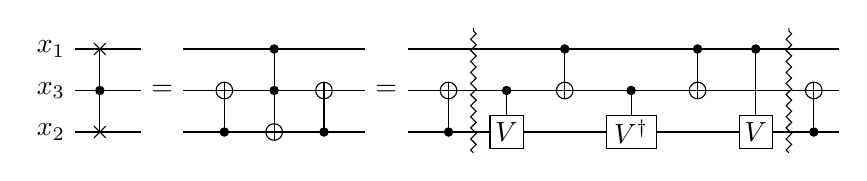
\begin{tikzpicture}[scale=1.000000,x=1pt,y=1pt]
\filldraw[color=white] (0.000000, -7.500000) rectangle (276.000000, 37.500000);
% Drawing wires
% Line 1: a3 W x_1
\draw[color=black] (0.000000,30.000000) -- (276.000000,30.000000);
\draw[color=black] (0.000000,30.000000) node[left] {$x_1$};
% Line 2: a2 W x_3
\draw[color=black] (0.000000,15.000000) -- (276.000000,15.000000);
\draw[color=black] (0.000000,15.000000) node[left] {$x_3$};
% Line 3: a1 W x_2
\draw[color=black] (0.000000,0.000000) -- (276.000000,0.000000);
\draw[color=black] (0.000000,0.000000) node[left] {$x_2$};
% Done with wires; drawing gates
% Line 4: a1 a3 SWAP a2
\draw (9.000000,30.000000) -- (9.000000,0.000000);
\begin{scope}
\draw (6.878680, -2.121320) -- (11.121320, 2.121320);
\draw (6.878680, 2.121320) -- (11.121320, -2.121320);
\end{scope}
\begin{scope}
\draw (6.878680, 27.878680) -- (11.121320, 32.121320);
\draw (6.878680, 32.121320) -- (11.121320, 27.878680);
\end{scope}
\filldraw (9.000000, 15.000000) circle(1.500000pt);
% Line 5: =
\draw[fill=white,color=white] (24.000000, -6.000000) rectangle (39.000000, 36.000000);
\draw (31.500000, 15.000000) node {$=$};
% Line 6: a1 +a2
\draw (54.000000,15.000000) -- (54.000000,0.000000);
\filldraw (54.000000, 0.000000) circle(1.500000pt);
\begin{scope}
\draw[fill=white] (54.000000, 15.000000) circle(3.000000pt);
\clip (54.000000, 15.000000) circle(3.000000pt);
\draw (51.000000, 15.000000) -- (57.000000, 15.000000);
\draw (54.000000, 12.000000) -- (54.000000, 18.000000);
\end{scope}
% Line 7: +a1 a2 a3
\draw (72.000000,30.000000) -- (72.000000,0.000000);
\begin{scope}
\draw[fill=white] (72.000000, 0.000000) circle(3.000000pt);
\clip (72.000000, 0.000000) circle(3.000000pt);
\draw (69.000000, 0.000000) -- (75.000000, 0.000000);
\draw (72.000000, -3.000000) -- (72.000000, 3.000000);
\end{scope}
\filldraw (72.000000, 15.000000) circle(1.500000pt);
\filldraw (72.000000, 30.000000) circle(1.500000pt);
% Line 8: a1 +a2
\draw (90.000000,15.000000) -- (90.000000,0.000000);
\filldraw (90.000000, 0.000000) circle(1.500000pt);
\begin{scope}
\draw[fill=white] (90.000000, 15.000000) circle(3.000000pt);
\clip (90.000000, 15.000000) circle(3.000000pt);
\draw (87.000000, 15.000000) -- (93.000000, 15.000000);
\draw (90.000000, 12.000000) -- (90.000000, 18.000000);
\end{scope}
% Line 9: =
\draw[fill=white,color=white] (105.000000, -6.000000) rectangle (120.000000, 36.000000);
\draw (112.500000, 15.000000) node {$=$};
% Line 10: a1 +a2
\draw (135.000000,15.000000) -- (135.000000,0.000000);
\filldraw (135.000000, 0.000000) circle(1.500000pt);
\begin{scope}
\draw[fill=white] (135.000000, 15.000000) circle(3.000000pt);
\clip (135.000000, 15.000000) circle(3.000000pt);
\draw (132.000000, 15.000000) -- (138.000000, 15.000000);
\draw (135.000000, 12.000000) -- (135.000000, 18.000000);
\end{scope}
% Line 11: BARRIER
\draw[decorate,decoration={zigzag,amplitude=1pt,segment length=4}] (144.000000,-7.500000) -- (144.000000,37.500000);
% Line 12: a1 G $V$ a2
\draw (156.000000,15.000000) -- (156.000000,0.000000);
\begin{scope}
\draw[fill=white] (156.000000, -0.000000) +(-45.000000:8.485281pt and 8.485281pt) -- +(45.000000:8.485281pt and 8.485281pt) -- +(135.000000:8.485281pt and 8.485281pt) -- +(225.000000:8.485281pt and 8.485281pt) -- cycle;
\clip (156.000000, -0.000000) +(-45.000000:8.485281pt and 8.485281pt) -- +(45.000000:8.485281pt and 8.485281pt) -- +(135.000000:8.485281pt and 8.485281pt) -- +(225.000000:8.485281pt and 8.485281pt) -- cycle;
\draw (156.000000, -0.000000) node {$V$};
\end{scope}
\filldraw (156.000000, 15.000000) circle(1.500000pt);
% Line 13: a3 +a2
\draw (177.000000,30.000000) -- (177.000000,15.000000);
\filldraw (177.000000, 30.000000) circle(1.500000pt);
\begin{scope}
\draw[fill=white] (177.000000, 15.000000) circle(3.000000pt);
\clip (177.000000, 15.000000) circle(3.000000pt);
\draw (174.000000, 15.000000) -- (180.000000, 15.000000);
\draw (177.000000, 12.000000) -- (177.000000, 18.000000);
\end{scope}
% Line 14: a1 G $V^\dagger$ a2 width=18
\draw (201.000000,15.000000) -- (201.000000,0.000000);
\begin{scope}
\draw[fill=white] (201.000000, -0.000000) +(-45.000000:12.727922pt and 8.485281pt) -- +(45.000000:12.727922pt and 8.485281pt) -- +(135.000000:12.727922pt and 8.485281pt) -- +(225.000000:12.727922pt and 8.485281pt) -- cycle;
\clip (201.000000, -0.000000) +(-45.000000:12.727922pt and 8.485281pt) -- +(45.000000:12.727922pt and 8.485281pt) -- +(135.000000:12.727922pt and 8.485281pt) -- +(225.000000:12.727922pt and 8.485281pt) -- cycle;
\draw (201.000000, -0.000000) node {$V^\dagger$};
\end{scope}
\filldraw (201.000000, 15.000000) circle(1.500000pt);
% Line 15: a3 +a2
\draw (225.000000,30.000000) -- (225.000000,15.000000);
\filldraw (225.000000, 30.000000) circle(1.500000pt);
\begin{scope}
\draw[fill=white] (225.000000, 15.000000) circle(3.000000pt);
\clip (225.000000, 15.000000) circle(3.000000pt);
\draw (222.000000, 15.000000) -- (228.000000, 15.000000);
\draw (225.000000, 12.000000) -- (225.000000, 18.000000);
\end{scope}
% Line 16: a1 G $V$ a3
\draw (246.000000,30.000000) -- (246.000000,0.000000);
\begin{scope}
\draw[fill=white] (246.000000, -0.000000) +(-45.000000:8.485281pt and 8.485281pt) -- +(45.000000:8.485281pt and 8.485281pt) -- +(135.000000:8.485281pt and 8.485281pt) -- +(225.000000:8.485281pt and 8.485281pt) -- cycle;
\clip (246.000000, -0.000000) +(-45.000000:8.485281pt and 8.485281pt) -- +(45.000000:8.485281pt and 8.485281pt) -- +(135.000000:8.485281pt and 8.485281pt) -- +(225.000000:8.485281pt and 8.485281pt) -- cycle;
\draw (246.000000, -0.000000) node {$V$};
\end{scope}
\filldraw (246.000000, 30.000000) circle(1.500000pt);
% Line 17: BARRIER
\draw[decorate,decoration={zigzag,amplitude=1pt,segment length=4}] (258.000000,-7.500000) -- (258.000000,37.500000);
% Line 18: a1 +a2
\draw (267.000000,15.000000) -- (267.000000,0.000000);
\filldraw (267.000000, 0.000000) circle(1.500000pt);
\begin{scope}
\draw[fill=white] (267.000000, 15.000000) circle(3.000000pt);
\clip (267.000000, 15.000000) circle(3.000000pt);
\draw (264.000000, 15.000000) -- (270.000000, 15.000000);
\draw (267.000000, 12.000000) -- (267.000000, 18.000000);
\end{scope}
% Done with gates; drawing ending labels
% Done with ending labels; drawing cut lines and comments
% Done with comments
\end{tikzpicture}
\end{center}
\vspace{-10pt}
This circuit contains 7 2-qubit gates, but consecutive applications of any 2-qubit gates to the same pair of qubits can be combined.  The resulting 2-qubit gate can likely not be thought of a  simple unitary applied to one of the qubits, controlled by the other though.  Still, combining the first two gates into a 2-qubit gate, say $G$, gives
\vspace{-5pt}
\begin{center}
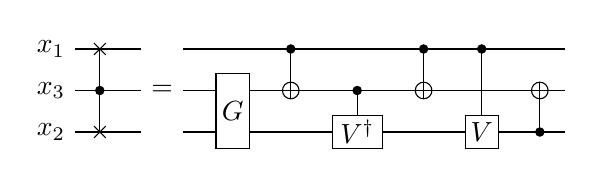
\begin{tikzpicture}[scale=1.000000,x=1pt,y=1pt]
\filldraw[color=white] (0.000000, -7.500000) rectangle (177.000000, 37.500000);
% Drawing wires
% Line 1: a3 W x_1
\draw[color=black] (0.000000,30.000000) -- (177.000000,30.000000);
\draw[color=black] (0.000000,30.000000) node[left] {$x_1$};
% Line 2: a2 W x_3
\draw[color=black] (0.000000,15.000000) -- (177.000000,15.000000);
\draw[color=black] (0.000000,15.000000) node[left] {$x_3$};
% Line 3: a1 W x_2
\draw[color=black] (0.000000,0.000000) -- (177.000000,0.000000);
\draw[color=black] (0.000000,0.000000) node[left] {$x_2$};
% Done with wires; drawing gates
% Line 4: a1 a3 SWAP a2
\draw (9.000000,30.000000) -- (9.000000,0.000000);
\begin{scope}
\draw (6.878680, -2.121320) -- (11.121320, 2.121320);
\draw (6.878680, 2.121320) -- (11.121320, -2.121320);
\end{scope}
\begin{scope}
\draw (6.878680, 27.878680) -- (11.121320, 32.121320);
\draw (6.878680, 32.121320) -- (11.121320, 27.878680);
\end{scope}
\filldraw (9.000000, 15.000000) circle(1.500000pt);
% Line 5: =
\draw[fill=white,color=white] (24.000000, -6.000000) rectangle (39.000000, 36.000000);
\draw (31.500000, 15.000000) node {$=$};
% Line 6: a1 a2 G $G$
\draw (57.000000,15.000000) -- (57.000000,0.000000);
\begin{scope}
\draw[fill=white] (57.000000, 7.500000) +(-45.000000:8.485281pt and 19.091883pt) -- +(45.000000:8.485281pt and 19.091883pt) -- +(135.000000:8.485281pt and 19.091883pt) -- +(225.000000:8.485281pt and 19.091883pt) -- cycle;
\clip (57.000000, 7.500000) +(-45.000000:8.485281pt and 19.091883pt) -- +(45.000000:8.485281pt and 19.091883pt) -- +(135.000000:8.485281pt and 19.091883pt) -- +(225.000000:8.485281pt and 19.091883pt) -- cycle;
\draw (57.000000, 7.500000) node {$G$};
\end{scope}
% Line 7: a3 +a2
\draw (78.000000,30.000000) -- (78.000000,15.000000);
\filldraw (78.000000, 30.000000) circle(1.500000pt);
\begin{scope}
\draw[fill=white] (78.000000, 15.000000) circle(3.000000pt);
\clip (78.000000, 15.000000) circle(3.000000pt);
\draw (75.000000, 15.000000) -- (81.000000, 15.000000);
\draw (78.000000, 12.000000) -- (78.000000, 18.000000);
\end{scope}
% Line 8: a1 G $V^\dagger$ a2 width=18
\draw (102.000000,15.000000) -- (102.000000,0.000000);
\begin{scope}
\draw[fill=white] (102.000000, -0.000000) +(-45.000000:12.727922pt and 8.485281pt) -- +(45.000000:12.727922pt and 8.485281pt) -- +(135.000000:12.727922pt and 8.485281pt) -- +(225.000000:12.727922pt and 8.485281pt) -- cycle;
\clip (102.000000, -0.000000) +(-45.000000:12.727922pt and 8.485281pt) -- +(45.000000:12.727922pt and 8.485281pt) -- +(135.000000:12.727922pt and 8.485281pt) -- +(225.000000:12.727922pt and 8.485281pt) -- cycle;
\draw (102.000000, -0.000000) node {$V^\dagger$};
\end{scope}
\filldraw (102.000000, 15.000000) circle(1.500000pt);
% Line 9: a3 +a2
\draw (126.000000,30.000000) -- (126.000000,15.000000);
\filldraw (126.000000, 30.000000) circle(1.500000pt);
\begin{scope}
\draw[fill=white] (126.000000, 15.000000) circle(3.000000pt);
\clip (126.000000, 15.000000) circle(3.000000pt);
\draw (123.000000, 15.000000) -- (129.000000, 15.000000);
\draw (126.000000, 12.000000) -- (126.000000, 18.000000);
\end{scope}
% Line 10: a1 G $V$ a3
\draw (147.000000,30.000000) -- (147.000000,0.000000);
\begin{scope}
\draw[fill=white] (147.000000, -0.000000) +(-45.000000:8.485281pt and 8.485281pt) -- +(45.000000:8.485281pt and 8.485281pt) -- +(135.000000:8.485281pt and 8.485281pt) -- +(225.000000:8.485281pt and 8.485281pt) -- cycle;
\clip (147.000000, -0.000000) +(-45.000000:8.485281pt and 8.485281pt) -- +(45.000000:8.485281pt and 8.485281pt) -- +(135.000000:8.485281pt and 8.485281pt) -- +(225.000000:8.485281pt and 8.485281pt) -- cycle;
\draw (147.000000, -0.000000) node {$V$};
\end{scope}
\filldraw (147.000000, 30.000000) circle(1.500000pt);
% Line 11: a1 +a2
\draw (168.000000,15.000000) -- (168.000000,0.000000);
\filldraw (168.000000, 0.000000) circle(1.500000pt);
\begin{scope}
\draw[fill=white] (168.000000, 15.000000) circle(3.000000pt);
\clip (168.000000, 15.000000) circle(3.000000pt);
\draw (165.000000, 15.000000) -- (171.000000, 15.000000);
\draw (168.000000, 12.000000) -- (168.000000, 18.000000);
\end{scope}
% Done with gates; drawing ending labels
% Done with ending labels; drawing cut lines and comments
% Done with comments
\end{tikzpicture}
\end{center}
\vspace{-10pt}
We answer part 4 in the negative in that, in the opinion of the second author, it is not worth removing another 2-qubit gate from the construction.  Arbitrary 2-qubit gates are likely to be extremely hard to implement in practice.  The controlled $V$ and $V^\dagger$ are likely to be hard as well, so in practice, instead of using the circuit in Figure 4.8, that in Figure 4.9 would likely be used, resulting in a circuit more along the lines of:
\begin{center}
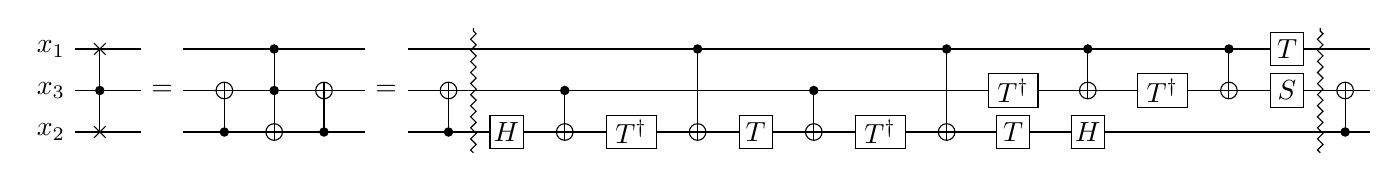
\begin{tikzpicture}[scale=1.000000,x=1pt,y=1pt]
\filldraw[color=white] (0.000000, -7.500000) rectangle (468.000000, 37.500000);
% Drawing wires
% Line 1: a3 W x_1
\draw[color=black] (0.000000,30.000000) -- (468.000000,30.000000);
\draw[color=black] (0.000000,30.000000) node[left] {$x_1$};
% Line 2: a2 W x_3
\draw[color=black] (0.000000,15.000000) -- (468.000000,15.000000);
\draw[color=black] (0.000000,15.000000) node[left] {$x_3$};
% Line 3: a1 W x_2
\draw[color=black] (0.000000,0.000000) -- (468.000000,0.000000);
\draw[color=black] (0.000000,0.000000) node[left] {$x_2$};
% Done with wires; drawing gates
% Line 4: a1 a3 SWAP a2
\draw (9.000000,30.000000) -- (9.000000,0.000000);
\begin{scope}
\draw (6.878680, -2.121320) -- (11.121320, 2.121320);
\draw (6.878680, 2.121320) -- (11.121320, -2.121320);
\end{scope}
\begin{scope}
\draw (6.878680, 27.878680) -- (11.121320, 32.121320);
\draw (6.878680, 32.121320) -- (11.121320, 27.878680);
\end{scope}
\filldraw (9.000000, 15.000000) circle(1.500000pt);
% Line 5: =
\draw[fill=white,color=white] (24.000000, -6.000000) rectangle (39.000000, 36.000000);
\draw (31.500000, 15.000000) node {$=$};
% Line 6: a1 +a2
\draw (54.000000,15.000000) -- (54.000000,0.000000);
\filldraw (54.000000, 0.000000) circle(1.500000pt);
\begin{scope}
\draw[fill=white] (54.000000, 15.000000) circle(3.000000pt);
\clip (54.000000, 15.000000) circle(3.000000pt);
\draw (51.000000, 15.000000) -- (57.000000, 15.000000);
\draw (54.000000, 12.000000) -- (54.000000, 18.000000);
\end{scope}
% Line 7: +a1 a2 a3
\draw (72.000000,30.000000) -- (72.000000,0.000000);
\begin{scope}
\draw[fill=white] (72.000000, 0.000000) circle(3.000000pt);
\clip (72.000000, 0.000000) circle(3.000000pt);
\draw (69.000000, 0.000000) -- (75.000000, 0.000000);
\draw (72.000000, -3.000000) -- (72.000000, 3.000000);
\end{scope}
\filldraw (72.000000, 15.000000) circle(1.500000pt);
\filldraw (72.000000, 30.000000) circle(1.500000pt);
% Line 8: a1 +a2
\draw (90.000000,15.000000) -- (90.000000,0.000000);
\filldraw (90.000000, 0.000000) circle(1.500000pt);
\begin{scope}
\draw[fill=white] (90.000000, 15.000000) circle(3.000000pt);
\clip (90.000000, 15.000000) circle(3.000000pt);
\draw (87.000000, 15.000000) -- (93.000000, 15.000000);
\draw (90.000000, 12.000000) -- (90.000000, 18.000000);
\end{scope}
% Line 9: =
\draw[fill=white,color=white] (105.000000, -6.000000) rectangle (120.000000, 36.000000);
\draw (112.500000, 15.000000) node {$=$};
% Line 10: a1 +a2
\draw (135.000000,15.000000) -- (135.000000,0.000000);
\filldraw (135.000000, 0.000000) circle(1.500000pt);
\begin{scope}
\draw[fill=white] (135.000000, 15.000000) circle(3.000000pt);
\clip (135.000000, 15.000000) circle(3.000000pt);
\draw (132.000000, 15.000000) -- (138.000000, 15.000000);
\draw (135.000000, 12.000000) -- (135.000000, 18.000000);
\end{scope}
% Line 11: BARRIER
\draw[decorate,decoration={zigzag,amplitude=1pt,segment length=4}] (144.000000,-7.500000) -- (144.000000,37.500000);
% Line 12: a1 H
\begin{scope}
\draw[fill=white] (156.000000, -0.000000) +(-45.000000:8.485281pt and 8.485281pt) -- +(45.000000:8.485281pt and 8.485281pt) -- +(135.000000:8.485281pt and 8.485281pt) -- +(225.000000:8.485281pt and 8.485281pt) -- cycle;
\clip (156.000000, -0.000000) +(-45.000000:8.485281pt and 8.485281pt) -- +(45.000000:8.485281pt and 8.485281pt) -- +(135.000000:8.485281pt and 8.485281pt) -- +(225.000000:8.485281pt and 8.485281pt) -- cycle;
\draw (156.000000, -0.000000) node {$H$};
\end{scope}
% Line 13: +a1 a2
\draw (177.000000,15.000000) -- (177.000000,0.000000);
\begin{scope}
\draw[fill=white] (177.000000, 0.000000) circle(3.000000pt);
\clip (177.000000, 0.000000) circle(3.000000pt);
\draw (174.000000, 0.000000) -- (180.000000, 0.000000);
\draw (177.000000, -3.000000) -- (177.000000, 3.000000);
\end{scope}
\filldraw (177.000000, 15.000000) circle(1.500000pt);
% Line 14: a1 G $T^\dagger$ width=18
\begin{scope}
\draw[fill=white] (201.000000, -0.000000) +(-45.000000:12.727922pt and 8.485281pt) -- +(45.000000:12.727922pt and 8.485281pt) -- +(135.000000:12.727922pt and 8.485281pt) -- +(225.000000:12.727922pt and 8.485281pt) -- cycle;
\clip (201.000000, -0.000000) +(-45.000000:12.727922pt and 8.485281pt) -- +(45.000000:12.727922pt and 8.485281pt) -- +(135.000000:12.727922pt and 8.485281pt) -- +(225.000000:12.727922pt and 8.485281pt) -- cycle;
\draw (201.000000, -0.000000) node {$T^\dagger$};
\end{scope}
% Line 15: +a1 a3
\draw (225.000000,30.000000) -- (225.000000,0.000000);
\begin{scope}
\draw[fill=white] (225.000000, 0.000000) circle(3.000000pt);
\clip (225.000000, 0.000000) circle(3.000000pt);
\draw (222.000000, 0.000000) -- (228.000000, 0.000000);
\draw (225.000000, -3.000000) -- (225.000000, 3.000000);
\end{scope}
\filldraw (225.000000, 30.000000) circle(1.500000pt);
% Line 16: a1 G $T$
\begin{scope}
\draw[fill=white] (246.000000, -0.000000) +(-45.000000:8.485281pt and 8.485281pt) -- +(45.000000:8.485281pt and 8.485281pt) -- +(135.000000:8.485281pt and 8.485281pt) -- +(225.000000:8.485281pt and 8.485281pt) -- cycle;
\clip (246.000000, -0.000000) +(-45.000000:8.485281pt and 8.485281pt) -- +(45.000000:8.485281pt and 8.485281pt) -- +(135.000000:8.485281pt and 8.485281pt) -- +(225.000000:8.485281pt and 8.485281pt) -- cycle;
\draw (246.000000, -0.000000) node {$T$};
\end{scope}
% Line 17: +a1 a2
\draw (267.000000,15.000000) -- (267.000000,0.000000);
\begin{scope}
\draw[fill=white] (267.000000, 0.000000) circle(3.000000pt);
\clip (267.000000, 0.000000) circle(3.000000pt);
\draw (264.000000, 0.000000) -- (270.000000, 0.000000);
\draw (267.000000, -3.000000) -- (267.000000, 3.000000);
\end{scope}
\filldraw (267.000000, 15.000000) circle(1.500000pt);
% Line 18: a1 G $T^\dagger$ width=18
\begin{scope}
\draw[fill=white] (291.000000, -0.000000) +(-45.000000:12.727922pt and 8.485281pt) -- +(45.000000:12.727922pt and 8.485281pt) -- +(135.000000:12.727922pt and 8.485281pt) -- +(225.000000:12.727922pt and 8.485281pt) -- cycle;
\clip (291.000000, -0.000000) +(-45.000000:12.727922pt and 8.485281pt) -- +(45.000000:12.727922pt and 8.485281pt) -- +(135.000000:12.727922pt and 8.485281pt) -- +(225.000000:12.727922pt and 8.485281pt) -- cycle;
\draw (291.000000, -0.000000) node {$T^\dagger$};
\end{scope}
% Line 19: +a1 a3
\draw (315.000000,30.000000) -- (315.000000,0.000000);
\begin{scope}
\draw[fill=white] (315.000000, 0.000000) circle(3.000000pt);
\clip (315.000000, 0.000000) circle(3.000000pt);
\draw (312.000000, 0.000000) -- (318.000000, 0.000000);
\draw (315.000000, -3.000000) -- (315.000000, 3.000000);
\end{scope}
\filldraw (315.000000, 30.000000) circle(1.500000pt);
% Line 20: TOUCH
% Line 21: a2 G $T^\dagger$ width=18
\begin{scope}
\draw[fill=white] (339.000000, 15.000000) +(-45.000000:12.727922pt and 8.485281pt) -- +(45.000000:12.727922pt and 8.485281pt) -- +(135.000000:12.727922pt and 8.485281pt) -- +(225.000000:12.727922pt and 8.485281pt) -- cycle;
\clip (339.000000, 15.000000) +(-45.000000:12.727922pt and 8.485281pt) -- +(45.000000:12.727922pt and 8.485281pt) -- +(135.000000:12.727922pt and 8.485281pt) -- +(225.000000:12.727922pt and 8.485281pt) -- cycle;
\draw (339.000000, 15.000000) node {$T^\dagger$};
\end{scope}
% Line 22: a1 G $T$
\begin{scope}
\draw[fill=white] (339.000000, -0.000000) +(-45.000000:8.485281pt and 8.485281pt) -- +(45.000000:8.485281pt and 8.485281pt) -- +(135.000000:8.485281pt and 8.485281pt) -- +(225.000000:8.485281pt and 8.485281pt) -- cycle;
\clip (339.000000, -0.000000) +(-45.000000:8.485281pt and 8.485281pt) -- +(45.000000:8.485281pt and 8.485281pt) -- +(135.000000:8.485281pt and 8.485281pt) -- +(225.000000:8.485281pt and 8.485281pt) -- cycle;
\draw (339.000000, -0.000000) node {$T$};
\end{scope}
% Line 23: a1 H
\begin{scope}
\draw[fill=white] (366.000000, -0.000000) +(-45.000000:8.485281pt and 8.485281pt) -- +(45.000000:8.485281pt and 8.485281pt) -- +(135.000000:8.485281pt and 8.485281pt) -- +(225.000000:8.485281pt and 8.485281pt) -- cycle;
\clip (366.000000, -0.000000) +(-45.000000:8.485281pt and 8.485281pt) -- +(45.000000:8.485281pt and 8.485281pt) -- +(135.000000:8.485281pt and 8.485281pt) -- +(225.000000:8.485281pt and 8.485281pt) -- cycle;
\draw (366.000000, -0.000000) node {$H$};
\end{scope}
% Line 24: +a2 a3
\draw (366.000000,30.000000) -- (366.000000,15.000000);
\begin{scope}
\draw[fill=white] (366.000000, 15.000000) circle(3.000000pt);
\clip (366.000000, 15.000000) circle(3.000000pt);
\draw (363.000000, 15.000000) -- (369.000000, 15.000000);
\draw (366.000000, 12.000000) -- (366.000000, 18.000000);
\end{scope}
\filldraw (366.000000, 30.000000) circle(1.500000pt);
% Line 25: a2 G $T^\dagger$ width=18
\begin{scope}
\draw[fill=white] (393.000000, 15.000000) +(-45.000000:12.727922pt and 8.485281pt) -- +(45.000000:12.727922pt and 8.485281pt) -- +(135.000000:12.727922pt and 8.485281pt) -- +(225.000000:12.727922pt and 8.485281pt) -- cycle;
\clip (393.000000, 15.000000) +(-45.000000:12.727922pt and 8.485281pt) -- +(45.000000:12.727922pt and 8.485281pt) -- +(135.000000:12.727922pt and 8.485281pt) -- +(225.000000:12.727922pt and 8.485281pt) -- cycle;
\draw (393.000000, 15.000000) node {$T^\dagger$};
\end{scope}
% Line 26: +a2 a3
\draw (417.000000,30.000000) -- (417.000000,15.000000);
\begin{scope}
\draw[fill=white] (417.000000, 15.000000) circle(3.000000pt);
\clip (417.000000, 15.000000) circle(3.000000pt);
\draw (414.000000, 15.000000) -- (420.000000, 15.000000);
\draw (417.000000, 12.000000) -- (417.000000, 18.000000);
\end{scope}
\filldraw (417.000000, 30.000000) circle(1.500000pt);
% Line 27: a3 G $T$
\begin{scope}
\draw[fill=white] (438.000000, 30.000000) +(-45.000000:8.485281pt and 8.485281pt) -- +(45.000000:8.485281pt and 8.485281pt) -- +(135.000000:8.485281pt and 8.485281pt) -- +(225.000000:8.485281pt and 8.485281pt) -- cycle;
\clip (438.000000, 30.000000) +(-45.000000:8.485281pt and 8.485281pt) -- +(45.000000:8.485281pt and 8.485281pt) -- +(135.000000:8.485281pt and 8.485281pt) -- +(225.000000:8.485281pt and 8.485281pt) -- cycle;
\draw (438.000000, 30.000000) node {$T$};
\end{scope}
% Line 28: a2 G $S$
\begin{scope}
\draw[fill=white] (438.000000, 15.000000) +(-45.000000:8.485281pt and 8.485281pt) -- +(45.000000:8.485281pt and 8.485281pt) -- +(135.000000:8.485281pt and 8.485281pt) -- +(225.000000:8.485281pt and 8.485281pt) -- cycle;
\clip (438.000000, 15.000000) +(-45.000000:8.485281pt and 8.485281pt) -- +(45.000000:8.485281pt and 8.485281pt) -- +(135.000000:8.485281pt and 8.485281pt) -- +(225.000000:8.485281pt and 8.485281pt) -- cycle;
\draw (438.000000, 15.000000) node {$S$};
\end{scope}
% Line 29: BARRIER
\draw[decorate,decoration={zigzag,amplitude=1pt,segment length=4}] (450.000000,-7.500000) -- (450.000000,37.500000);
% Line 30: a1 +a2
\draw (459.000000,15.000000) -- (459.000000,0.000000);
\filldraw (459.000000, 0.000000) circle(1.500000pt);
\begin{scope}
\draw[fill=white] (459.000000, 15.000000) circle(3.000000pt);
\clip (459.000000, 15.000000) circle(3.000000pt);
\draw (456.000000, 15.000000) -- (462.000000, 15.000000);
\draw (459.000000, 12.000000) -- (459.000000, 18.000000);
\end{scope}
% Done with gates; drawing ending labels
% Done with ending labels; drawing cut lines and comments
% Done with comments
\end{tikzpicture}
\end{center}
\vspace{-10pt}
Gates 0-3 could be combined into a single 2-qubit gate, but likely would not be in practice due to implementation difficulty.
\newpage
\Textbf{4.26} Show that the circuit:
\begin{center}
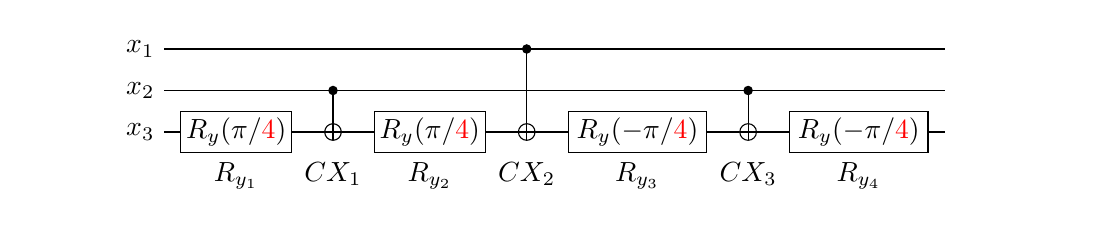
\begin{tikzpicture}[scale=1.000000,x=1pt,y=1pt]
\filldraw[color=white] (0.000000, -7.500000) rectangle (282.000000, 37.500000);
% Drawing wires
% Line 1: a3 W x_3
\draw[color=black] (0.000000,30.000000) -- (282.000000,30.000000);
\draw[color=black] (0.000000,30.000000) node[left] {$x_1$};
% Line 2: a2 W x_2
\draw[color=black] (0.000000,15.000000) -- (282.000000,15.000000);
\draw[color=black] (0.000000,15.000000) node[left] {$x_2$};
% Line 3: a1 W x_1
\draw[color=black] (0.000000,0.000000) -- (282.000000,0.000000);
\draw[color=black] (0.000000,0.000000) node[left] {$x_3$};
% Done with wires; drawing gates
% Line 4: a1 G $R_y(\pi/\textcolor{red}{4})$ width=40 height=15 %% $R_{y_1}$
\draw (26.000000, -7.500000) node[text width=144pt,below,text centered] {$R_{y_1}$};
\begin{scope}
\draw[fill=white] (26.000000, -0.000000) +(-45.000000:28.284271pt and 10.606602pt) -- +(45.000000:28.284271pt and 10.606602pt) -- +(135.000000:28.284271pt and 10.606602pt) -- +(225.000000:28.284271pt and 10.606602pt) -- cycle;
\clip (26.000000, -0.000000) +(-45.000000:28.284271pt and 10.606602pt) -- +(45.000000:28.284271pt and 10.606602pt) -- +(135.000000:28.284271pt and 10.606602pt) -- +(225.000000:28.284271pt and 10.606602pt) -- cycle;
\draw (26.000000, -0.000000) node {$R_y(\pi/\textcolor{red}{4})$};
\end{scope}
% Line 5: +a1 a2 %% $CX_1$
\draw (61.000000, -7.500000) node[text width=144pt,below,text centered] {$CX_1$};
\draw (61.000000,15.000000) -- (61.000000,0.000000);
\begin{scope}
\draw[fill=white] (61.000000, 0.000000) circle(3.000000pt);
\clip (61.000000, 0.000000) circle(3.000000pt);
\draw (58.000000, 0.000000) -- (64.000000, 0.000000);
\draw (61.000000, -3.000000) -- (61.000000, 3.000000);
\end{scope}
\filldraw (61.000000, 15.000000) circle(1.500000pt);
% Line 6: a1 G $R_y(\pi/\textcolor{red}{4})$ width=40 height=15 %% $R_{y_2}$
\draw (96.000000, -7.500000) node[text width=144pt,below,text centered] {$R_{y_2}$};
\begin{scope}
\draw[fill=white] (96.000000, -0.000000) +(-45.000000:28.284271pt and 10.606602pt) -- +(45.000000:28.284271pt and 10.606602pt) -- +(135.000000:28.284271pt and 10.606602pt) -- +(225.000000:28.284271pt and 10.606602pt) -- cycle;
\clip (96.000000, -0.000000) +(-45.000000:28.284271pt and 10.606602pt) -- +(45.000000:28.284271pt and 10.606602pt) -- +(135.000000:28.284271pt and 10.606602pt) -- +(225.000000:28.284271pt and 10.606602pt) -- cycle;
\draw (96.000000, -0.000000) node {$R_y(\pi/\textcolor{red}{4})$};
\end{scope}
% Line 7: +a1 a3 %% $CX_2$
\draw (131.000000, -7.500000) node[text width=144pt,below,text centered] {$CX_2$};
\draw (131.000000,30.000000) -- (131.000000,0.000000);
\begin{scope}
\draw[fill=white] (131.000000, 0.000000) circle(3.000000pt);
\clip (131.000000, 0.000000) circle(3.000000pt);
\draw (128.000000, 0.000000) -- (134.000000, 0.000000);
\draw (131.000000, -3.000000) -- (131.000000, 3.000000);
\end{scope}
\filldraw (131.000000, 30.000000) circle(1.500000pt);
% Line 8: a1 G $R_y(-\pi/\textcolor{red}{4})$ width=50 height=15 %% $R_{y_3}$
\draw (171.000000, -7.500000) node[text width=144pt,below,text centered] {$R_{y_3}$};
\begin{scope}
\draw[fill=white] (171.000000, -0.000000) +(-45.000000:35.355339pt and 10.606602pt) -- +(45.000000:35.355339pt and 10.606602pt) -- +(135.000000:35.355339pt and 10.606602pt) -- +(225.000000:35.355339pt and 10.606602pt) -- cycle;
\clip (171.000000, -0.000000) +(-45.000000:35.355339pt and 10.606602pt) -- +(45.000000:35.355339pt and 10.606602pt) -- +(135.000000:35.355339pt and 10.606602pt) -- +(225.000000:35.355339pt and 10.606602pt) -- cycle;
\draw (171.000000, -0.000000) node {$R_y(-\pi/\textcolor{red}{4})$};
\end{scope}
% Line 9: +a1 a2 %% $CX_3$
\draw (211.000000, -7.500000) node[text width=144pt,below,text centered] {$CX_3$};
\draw (211.000000,15.000000) -- (211.000000,0.000000);
\begin{scope}
\draw[fill=white] (211.000000, 0.000000) circle(3.000000pt);
\clip (211.000000, 0.000000) circle(3.000000pt);
\draw (208.000000, 0.000000) -- (214.000000, 0.000000);
\draw (211.000000, -3.000000) -- (211.000000, 3.000000);
\end{scope}
\filldraw (211.000000, 15.000000) circle(1.500000pt);
% Line 10: a1 G $R_y(-\pi/\textcolor{red}{4})$ width=50 height=15 %% $R_{y_4}$
\draw (251.000000, -7.500000) node[text width=144pt,below,text centered] {$R_{y_4}$};
\begin{scope}
\draw[fill=white] (251.000000, -0.000000) +(-45.000000:35.355339pt and 10.606602pt) -- +(45.000000:35.355339pt and 10.606602pt) -- +(135.000000:35.355339pt and 10.606602pt) -- +(225.000000:35.355339pt and 10.606602pt) -- cycle;
\clip (251.000000, -0.000000) +(-45.000000:35.355339pt and 10.606602pt) -- +(45.000000:35.355339pt and 10.606602pt) -- +(135.000000:35.355339pt and 10.606602pt) -- +(225.000000:35.355339pt and 10.606602pt) -- cycle;
\draw (251.000000, -0.000000) node {$R_y(-\pi/\textcolor{red}{4})$};
\end{scope}
% Done with gates; drawing ending labels
% Done with ending labels; drawing cut lines and comments
% Done with comments
\end{tikzpicture}
\end{center}
\vspace{-5pt}
differs from a Toffoli gate only by relative phases.  That is, the circuit takes $\ket{c_1, c_2, t}$ to $e^{i\theta(c_1,c_2,t)}\cdot \ket{c_1,c_2,t\oplus c_1\cdot c_2}$, where $e^{i\theta(c_1,c_2,t)}$ is some relative phase factor. Such gates can sometimes be useful in experimental implementations, where it may be much easier to implement a gate that is the same as the Toffoli up to relative phases than it is to do the Toffoli directly.
\begin{comment}
\Soln Note that $R_y(\pm\pi) = \mp iY = \begin{bmatrix} 0 & \mp1 \\ \pm 1 & 0 \end{bmatrix}$, which maps $\ket{0} \rightarrow \pm \ket{1}$ and $\ket{1}\rightarrow\mp\ket{0}$. Now, we trace the effects of the circuit on the computational basis.
\vspace{-10pt}
\begin{center}
\begin{tabular}{c|r|r|r|r|r|r|r|} 
\multicolumn{1}{c|}{$\ket{x_1x_2x_3}$} & \multicolumn{1}{c|}{$R_{y_1}$} & \multicolumn{1}{c|}{$CX_1$} & \multicolumn{1}{c|}{$R_{y_2}$ } & \multicolumn{1}{c|}{$CX_2$} & \multicolumn{1}{c|}{$R_{y_3}$ } & \multicolumn{1}{c|}{$CX_3$} & \multicolumn{1}{c|}{$R_{y_4}$} \\
\hline
$\ket{000}$ & $\ket{001}$ & $\ket{001}$ & $-\ket{000}$ & $-\ket{000}$ & $\ket{001}$ & $\ket{001}$ & $\ket{000}$ \\
\hline
$\ket{001}$ & $-\ket{000}$ & $-\ket{000}$ & $-\ket{001}$ & $-\ket{001}$ & $-\ket{000}$ & $-\ket{000}$ & $\ket{001}$ \\
\hline
$\ket{010}$ & $\ket{011}$ & $\ket{010}$ & $\ket{011}$ & $\ket{011}$ & $\ket{010}$ & $\ket{011}$ & $\ket{010}$ \\
\hline
$\ket{011}$ & $-\ket{010}$ & $-\ket{011}$ & $\ket{010}$ & $\ket{010}$ & $-\ket{011}$ & $-\ket{010}$ & $\ket{011}$ \\
\hline
$\ket{100}$ & $\ket{101}$ & $\ket{101}$ & $-\ket{100}$ & $-\ket{101}$ & $-\ket{100}$ & $-\ket{100}$ & $\ket{101}$ \\
\hline
$\ket{101}$ & $-\ket{100}$ & $-\ket{100}$ & $-\ket{101}$ & $-\ket{100}$ & $\ket{101}$ & $\ket{101}$ & $\ket{100}$ \\
\hline
$\ket{110}$ & $\ket{111}$ & $\ket{110}$ & $\ket{111}$ & $\ket{110}$ & $-\ket{111}$ & $-\ket{110}$ & $\ket{111}$ \\
\hline
$\ket{111}$ & $-\ket{110}$ & $-\ket{111}$ & $\ket{110}$  & $\ket{111}$ & $\ket{110}$ & $\ket{111}$ & $\ket{110}$ 
\end{tabular}
\end{center}
\vspace{-10pt}
That didn't work out ... it incorrectly maps $\ket{100}\rightarrow\ket{101}$ and $\ket{100}\rightarrow{101}$, effectively, this is just \CNOT$(x_1,x_3)$.
\end{comment}
\Soln Note the correction changing the rotations to $\pi/4$ instead of $\pi$.  Using rotations of $\pi$, the circuit is equivalent to a single \CNOT$(x_1, x_3)$.  Now, none of the gates alter the states of $\ket{x_1}$ or $\ket{x_2}$, so we can analyze this circuit by focusing only on it's effect on $\ket{x_3}$ while conditioning on the static state of $\ket{x_1x_2}$. First, we'll expand $R_y(\pm\pi/4)$.  Note that $\cos(\pm\pi/8) = \frac{\sqrt{2+\sqrt{2}}}{2}$, and $\sin(\pm\pi/8)=\pm\frac{\sqrt{2-\sqrt{2}}}{2}$.  Now:
$$R_y(\pm\pi/4) = \cos(\pm\pi/8)I-i\sin(\pm\pi/8)Y = \begin{bmatrix}\cos(\pm\pi/8) & -\sin(\pm\pi/8) \\ \sin(\pm\pi/8)& \cos(\pm\pi/8)\end{bmatrix} = \begin{bmatrix} \frac{\sqrt{2+\sqrt{2}}}{2} & \mp\frac{\sqrt{2-\sqrt{2}}}{2} \\ \pm\frac{\sqrt{2-\sqrt{2}}}{2} & \frac{\sqrt{2+\sqrt{2}}}{2}\end{bmatrix}.$$

When $\ket{x_1x_2}=\ket{00}$, the operations applied to $\ket{x_3}$ are $R_y(\pi/4)^2R_y(-\pi/4)^2$.  Note that $R_y(\theta)R_y(-\theta) = I$, so in this case the circuit does not change the state of $\ket{x_3}$.  When $\ket{x_1x_2} = \ket{01}$, the operations applied to $\ket{x_3}$ are $R_y(\pi/8)XR_y(\pi/8)R_y(-\pi/8)XR_y(-\pi/8)=R_y(\pi/8)X^2R_y*(-\pi/8)=R_y(\pi/8)R_y*(-\pi/8)=I$, so again, $\ket{x_3}$ is unchanged.  When $\ket{x_1x_2} = \ket{10}$, the operations are:
\begin{align*}
R_y(\pi/4)^2XR_y(-\pi/4)^2 &= R_y(\pi/2)XR_y(-\pi/2) \\
                           &= \begin{bmatrix}\frac{\sqrt{2}}{2} & - \frac{\sqrt{2}}{2} \\ \frac{\sqrt{2}}{2} &  \frac{\sqrt{2}}{2}\end{bmatrix}
                              \begin{bmatrix} 0 & 1 \\ 1 & 0 \end{bmatrix}
                              \begin{bmatrix}\frac{\sqrt{2}}{2} & \frac{\sqrt{2}}{2} \\ -\frac{\sqrt{2}}{2} &  \frac{\sqrt{2}}{2}\end{bmatrix} \\
                           &= \begin{bmatrix} -1 & 0 \\ 0 & 1\end{bmatrix}
\end{align*}
Finally, when $\ket{x_1x_2} = \ket{11}$, the operations are:
$$R_y(\pi/4)XR_y(\pi/4)XR_y(-\pi/4)XR_y(-\pi/4) = $$
$$\begin{bmatrix} \frac{\sqrt{2+\sqrt{2}}}{2} & -\frac{\sqrt{2-\sqrt{2}}}{2} \\ \frac{\sqrt{2-\sqrt{2}}}{2} & \frac{\sqrt{2+\sqrt{2}}}{2} \end{bmatrix}
\begin{bmatrix} 0 & 1 \\ 1 & 0 \end{bmatrix} 
\begin{bmatrix} \frac{\sqrt{2+\sqrt{2}}}{2} & -\frac{\sqrt{2-\sqrt{2}}}{2} \\ \frac{\sqrt{2-\sqrt{2}}}{2} & \frac{\sqrt{2+\sqrt{2}}}{2}\end{bmatrix}
\begin{bmatrix} 0 & 1 \\ 1 & 0 \end{bmatrix}
\begin{bmatrix} \frac{\sqrt{2+\sqrt{2}}}{2} & \frac{\sqrt{2-\sqrt{2}}}{2} \\ -\frac{\sqrt{2-\sqrt{2}}}{2} & \frac{\sqrt{2+\sqrt{2}}}{2}\end{bmatrix}
\begin{bmatrix} 0 & 1 \\ 1 & 0 \end{bmatrix}
\begin{bmatrix} \frac{\sqrt{2+\sqrt{2}}}{2} & \frac{\sqrt{2-\sqrt{2}}}{2} \\ -\frac{\sqrt{2-\sqrt{2}}}{2} & \frac{\sqrt{2+\sqrt{2}}}{2}\end{bmatrix} $$
$$= \begin{bmatrix} 0 & 1 \\ 1 & 0\end{bmatrix} = X$$


So, the circuit performs the transformation $$\begin{bmatrix}
1 & 0 & 0 & 0 & 0 & 0 & 0 & 0 \\
0 & 1 & 0 & 0 & 0 & 0 & 0 & 0 \\
0 & 0 & 1 & 0 & 0 & 0 & 0 & 0 \\
0 & 0 & 0 & 1 & 0 & 0 & 0 & 0 \\
0 & 0 & 0 & 0 & -1 & 0 & 0 & 0 \\
0 & 0 & 0 & 0 & 0 & 1 & 0 & 0 \\
0 & 0 & 0 & 0 & 0 & 0 & 0 & 1 \\
0 & 0 & 0 & 0 & 0 & 0 & 1 & 0 \\
\end{bmatrix}$$
This transformation matches a Toffoli gate, except that it introduces a relative phase of $\pi$ to the result of the computational basis state $\ket{100}$.

\Textbf{4.27} Using just \CNOT s and Toffoli gates, construct a quantum circuit to perform the tansformation
$$\pi = \begin{bmatrix}
1 & 0 & 0 & 0 & 0 & 0 & 0 & 0 \\
0 & 0 & 0 & 0 & 0 & 0 & 0 & 1 \\
0 & 1 & 0 & 0 & 0 & 0 & 0 & 0 \\
0 & 0 & 1 & 0 & 0 & 0 & 0 & 0 \\
0 & 0 & 0 & 1 & 0 & 0 & 0 & 0 \\
0 & 0 & 0 & 0 & 1 & 0 & 0 & 0 \\
0 & 0 & 0 & 0 & 0 & 1 & 0 & 0 \\
0 & 0 & 0 & 0 & 0 & 0 & 1 & 0 \\
\end{bmatrix}$$
This kind of partial cyclic permutation operation will be useful later, in Chapter 7.
\Soln \CNOT s and Toffoli gates permute the computational basis states as does the target transformation. But for lack of intuition, a python script was written to exhaustively search products of the permutations they represent, looking for the target transformation as the result.  A product of 5 gates was found involving 2 Toffolis and 3 \CNOT s:
\begin{center}\ \ \ \ \ \ \ \ 
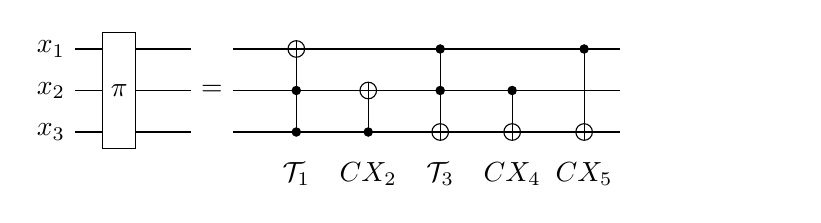
\begin{tikzpicture}[scale=1.000000,x=1pt,y=1pt]
\filldraw[color=white] (0.000000, -7.500000) rectangle (197.000000, 37.500000);
% Drawing wires
% Line 1: a1 W x_1
\draw[color=black] (0.000000,30.000000) -- (197.000000,30.000000);
\draw[color=black] (0.000000,30.000000) node[left] {$x_1$};
% Line 2: a2 W x_2
\draw[color=black] (0.000000,15.000000) -- (197.000000,15.000000);
\draw[color=black] (0.000000,15.000000) node[left] {$x_2$};
% Line 3: a3 W x_3
\draw[color=black] (0.000000,0.000000) -- (197.000000,0.000000);
\draw[color=black] (0.000000,0.000000) node[left] {$x_3$};
% Done with wires; drawing gates
% Line 4: a1 a2 a3 G $\pi$
\draw (16.000000,30.000000) -- (16.000000,0.000000);
\begin{scope}
\draw[fill=white] (16.000000, 15.000000) +(-45.000000:8.485281pt and 29.698485pt) -- +(45.000000:8.485281pt and 29.698485pt) -- +(135.000000:8.485281pt and 29.698485pt) -- +(225.000000:8.485281pt and 29.698485pt) -- cycle;
\clip (16.000000, 15.000000) +(-45.000000:8.485281pt and 29.698485pt) -- +(45.000000:8.485281pt and 29.698485pt) -- +(135.000000:8.485281pt and 29.698485pt) -- +(225.000000:8.485281pt and 29.698485pt) -- cycle;
\draw (16.000000, 15.000000) node {$\pi$};
\end{scope}
% Line 5: =
\draw[fill=white,color=white] (42.000000, -6.000000) rectangle (57.000000, 36.000000);
\draw (49.500000, 15.000000) node {$=$};
% Line 6: +a1 a2 a3 %% $\mathcal{T}_1$
\draw (80.000000, -7.500000) node[text width=144pt,below,text centered] {$\mathcal{T}_1$};
\draw (80.000000,30.000000) -- (80.000000,0.000000);
\begin{scope}
\draw[fill=white] (80.000000, 30.000000) circle(3.000000pt);
\clip (80.000000, 30.000000) circle(3.000000pt);
\draw (77.000000, 30.000000) -- (83.000000, 30.000000);
\draw (80.000000, 27.000000) -- (80.000000, 33.000000);
\end{scope}
\filldraw (80.000000, 15.000000) circle(1.500000pt);
\filldraw (80.000000, 0.000000) circle(1.500000pt);
% Line 7: +a2 a3 %% $CX_2$
\draw (106.000000, -7.500000) node[text width=144pt,below,text centered] {$CX_2$};
\draw (106.000000,15.000000) -- (106.000000,0.000000);
\begin{scope}
\draw[fill=white] (106.000000, 15.000000) circle(3.000000pt);
\clip (106.000000, 15.000000) circle(3.000000pt);
\draw (103.000000, 15.000000) -- (109.000000, 15.000000);
\draw (106.000000, 12.000000) -- (106.000000, 18.000000);
\end{scope}
\filldraw (106.000000, 0.000000) circle(1.500000pt);
% Line 8: +a3 a1 a2 %% $\mathcal{T}_3$
\draw (132.000000, -7.500000) node[text width=144pt,below,text centered] {$\mathcal{T}_3$};
\draw (132.000000,30.000000) -- (132.000000,0.000000);
\begin{scope}
\draw[fill=white] (132.000000, 0.000000) circle(3.000000pt);
\clip (132.000000, 0.000000) circle(3.000000pt);
\draw (129.000000, 0.000000) -- (135.000000, 0.000000);
\draw (132.000000, -3.000000) -- (132.000000, 3.000000);
\end{scope}
\filldraw (132.000000, 30.000000) circle(1.500000pt);
\filldraw (132.000000, 15.000000) circle(1.500000pt);
% Line 9: +a3 a2 %% $CX_4$
\draw (158.000000, -7.500000) node[text width=144pt,below,text centered] {$CX_4$};
\draw (158.000000,15.000000) -- (158.000000,0.000000);
\begin{scope}
\draw[fill=white] (158.000000, 0.000000) circle(3.000000pt);
\clip (158.000000, 0.000000) circle(3.000000pt);
\draw (155.000000, 0.000000) -- (161.000000, 0.000000);
\draw (158.000000, -3.000000) -- (158.000000, 3.000000);
\end{scope}
\filldraw (158.000000, 15.000000) circle(1.500000pt);
% Line 10: +a3 a1 %% $CX_5$
\draw (184.000000, -7.500000) node[text width=144pt,below,text centered] {$CX_5$};
\draw (184.000000,30.000000) -- (184.000000,0.000000);
\begin{scope}
\draw[fill=white] (184.000000, 0.000000) circle(3.000000pt);
\clip (184.000000, 0.000000) circle(3.000000pt);
\draw (181.000000, 0.000000) -- (187.000000, 0.000000);
\draw (184.000000, -3.000000) -- (184.000000, 3.000000);
\end{scope}
\filldraw (184.000000, 30.000000) circle(1.500000pt);
% Done with gates; drawing ending labels
% Done with ending labels; drawing cut lines and comments
% Done with comments
\end{tikzpicture}
\end{center}
\vspace{-15pt}
\begin{center}
\begin{tabular}{c|c|c|c|c|c|} 
$\ket{x_1x_2x_3}$ & $\mathcal{T}_1$ & $CX_2$ & $\mathcal{T}_3$ & $CX_4$ & $CX_5$\\
\hline
$\ket{000}$ & $\ket{000}$ & $\ket{000}$ & $\ket{000}$ & $\ket{000}$ & $\ket{000}$ \\
\hline
$\ket{001}$  & $\ket{001}$ & $\ket{011}$ & $\ket{011}$ & $\ket{010}$ & $\ket{010}$  \\
\hline
$\ket{010}$ & $\ket{010}$ & $\ket{010}$ & $\ket{010}$ & $\ket{011}$ & $\ket{011}$ \\
\hline
$\ket{011}$ & $\ket{111}$ & $\ket{101}$ & $\ket{101}$ & $\ket{101}$ & $\ket{100}$ \\
\hline
$\ket{100}$ & $\ket{100}$ & $\ket{100}$ & $\ket{100}$ & $\ket{100}$ & $\ket{101}$ \\
\hline
$\ket{101}$ & $\ket{101}$ & $\ket{111}$ & $\ket{110}$ & $\ket{111}$ & $\ket{110}$ \\
\hline
$\ket{110}$ & $\ket{110}$ & $\ket{110}$ & $\ket{111}$ & $\ket{110}$ & $\ket{111}$ \\
\hline
$\ket{111}$ & $\ket{011}$ & $\ket{001}$ & $\ket{001}$ & $\ket{001}$ & $\ket{001}$ 
\end{tabular}
\end{center}
\vspace{-10pt}
The last 3 gates effectively execute a \NOT\ on $\ket{x_3}$ if $\ket{x_1}=\ket{1}$ \textit{and/or} $\ket{x_2}=\ket{1}$.  They can be performed in any order, leading to 6 equivalent circuits realizing $\pi$.  These 6 are the only ``minimal realizations'', that is, the only circuits realizing $\pi$ using the least Toffolis and/or \CNOT s possible.  

In an effort to determine which permutations could be implemented via Toffolis and \CNOT s, the script was used to tabulate the number of permutations minimally representable as products of these gates of various lengths.  Because the usable gates are all controlled and no controlled gate alters the state $\ket{000}$, all products of such gates fix $\ket{000}$.  There are $7!=5040$ permutations of the remaining computation basis states, so there are potentially 5040 permutations of the computational basis that could be represented.  Suprisingly, at least to the second author, all of them are representable.  The following table lists counts of the minimum number of required gates:
\begin{center}
\begin{tabular}{|c|r|}
 gates & \multicolumn{1}{c|}{count} \\ \hline
0 & 1 \\ \hline
1 & 9 \\ \hline
2 & 60 \\ \hline
3 & 261 \\ \hline
4 & 845 \\ \hline
5 & 1784 \\ \hline
6 & 1688 \\ \hline
7 & 386 \\ \hline
8 & 6
\end{tabular}
\end{center}
\vspace{-5pt} The unique permutation representable as a product of 0 \CNOT s and/or Toffolis is, of course, the identity.  The 9 representable as products of single gates are the gates themselves.  There are $9^2=81$ possible products of two gates, 9 of which consist of a repeated gate and so produce the identity.  There are 3 types of symmetries that cause 12 of the 81 pairs to produce the same non-identity result, so the 81 pairs ultimately only produce 60 dinstinct permutations as products of 2 \CNOT s and/or Toffolis.  The symmetries are depicted below.
\begin{center}
\ \ \ \ 
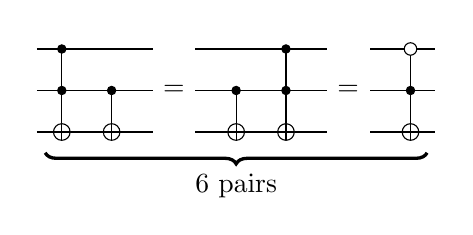
\begin{tikzpicture}[scale=1.000000,x=1pt,y=1pt]
\filldraw[color=white] (0.000000, -7.500000) rectangle (144.000000, 37.500000);
% Drawing wires
% Line 1: a1 W
\draw[color=black] (0.000000,30.000000) -- (144.000000,30.000000);
% Line 2: a2 W
\draw[color=black] (0.000000,15.000000) -- (144.000000,15.000000);
% Line 3: a3 W
\draw[color=black] (0.000000,0.000000) -- (144.000000,0.000000);
% Done with wires; drawing gates
% Line 4: a1 a2 +a3
\draw (9.000000,30.000000) -- (9.000000,0.000000);
\filldraw (9.000000, 30.000000) circle(1.500000pt);
\filldraw (9.000000, 15.000000) circle(1.500000pt);
\begin{scope}
\draw[fill=white] (9.000000, 0.000000) circle(3.000000pt);
\clip (9.000000, 0.000000) circle(3.000000pt);
\draw (6.000000, 0.000000) -- (12.000000, 0.000000);
\draw (9.000000, -3.000000) -- (9.000000, 3.000000);
\end{scope}
% Line 5: a2 +a3
\draw (27.000000,15.000000) -- (27.000000,0.000000);
\filldraw (27.000000, 15.000000) circle(1.500000pt);
\begin{scope}
\draw[fill=white] (27.000000, 0.000000) circle(3.000000pt);
\clip (27.000000, 0.000000) circle(3.000000pt);
\draw (24.000000, 0.000000) -- (30.000000, 0.000000);
\draw (27.000000, -3.000000) -- (27.000000, 3.000000);
\end{scope}
% Line 6: =
\draw[fill=white,color=white] (42.000000, -6.000000) rectangle (57.000000, 36.000000);
\draw (49.500000, 15.000000) node {$=$};
% Line 7: a2 +a3
\draw (72.000000,15.000000) -- (72.000000,0.000000);
\filldraw (72.000000, 15.000000) circle(1.500000pt);
\begin{scope}
\draw[fill=white] (72.000000, 0.000000) circle(3.000000pt);
\clip (72.000000, 0.000000) circle(3.000000pt);
\draw (69.000000, 0.000000) -- (75.000000, 0.000000);
\draw (72.000000, -3.000000) -- (72.000000, 3.000000);
\end{scope}
% Line 8: a1 a2 +a3
\draw (90.000000,30.000000) -- (90.000000,0.000000);
\filldraw (90.000000, 30.000000) circle(1.500000pt);
\filldraw (90.000000, 15.000000) circle(1.500000pt);
\begin{scope}
\draw[fill=white] (90.000000, 0.000000) circle(3.000000pt);
\clip (90.000000, 0.000000) circle(3.000000pt);
\draw (87.000000, 0.000000) -- (93.000000, 0.000000);
\draw (90.000000, -3.000000) -- (90.000000, 3.000000);
\end{scope}
% Line 9: =
\draw[fill=white,color=white] (105.000000, -6.000000) rectangle (120.000000, 36.000000);
\draw (112.500000, 15.000000) node {$=$};
% Line 10: -a1 a2 +a3
\draw (135.000000,30.000000) -- (135.000000,0.000000);
\draw[fill=white] (135.000000, 30.000000) circle(2.250000pt);
\filldraw (135.000000, 15.000000) circle(1.500000pt);
\begin{scope}
\draw[fill=white] (135.000000, 0.000000) circle(3.000000pt);
\clip (135.000000, 0.000000) circle(3.000000pt);
\draw (132.000000, 0.000000) -- (138.000000, 0.000000);
\draw (135.000000, -3.000000) -- (135.000000, 3.000000);
\end{scope}
% Done with gates; drawing ending labels
% Done with ending labels; drawing cut lines and comments
% Line 11: @ 7 %% 6 pairs
\draw[decorate,decoration={brace,mirror,amplitude = 4.000000pt},very thick] (3.000000,-7.500000) -- (141.000000,-7.500000);
\draw (72.000000, -11.500000) node[text width=144pt,below,text centered] {6 pairs};
% Done with comments
\end{tikzpicture}
\ \ \ \ \ \ 
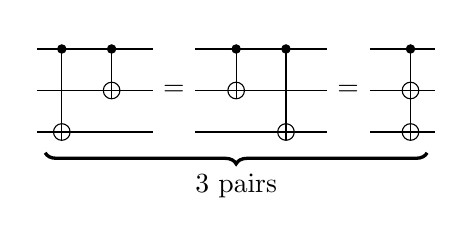
\begin{tikzpicture}[scale=1.000000,x=1pt,y=1pt]
\filldraw[color=white] (0.000000, -7.500000) rectangle (144.000000, 37.500000);
% Drawing wires
% Line 1: a1 W
\draw[color=black] (0.000000,30.000000) -- (144.000000,30.000000);
% Line 2: a2 W
\draw[color=black] (0.000000,15.000000) -- (144.000000,15.000000);
% Line 3: a3 W
\draw[color=black] (0.000000,0.000000) -- (144.000000,0.000000);
% Done with wires; drawing gates
% Line 4: a1 +a3
\draw (9.000000,30.000000) -- (9.000000,0.000000);
\filldraw (9.000000, 30.000000) circle(1.500000pt);
\begin{scope}
\draw[fill=white] (9.000000, 0.000000) circle(3.000000pt);
\clip (9.000000, 0.000000) circle(3.000000pt);
\draw (6.000000, 0.000000) -- (12.000000, 0.000000);
\draw (9.000000, -3.000000) -- (9.000000, 3.000000);
\end{scope}
% Line 5: a1 +a2
\draw (27.000000,30.000000) -- (27.000000,15.000000);
\filldraw (27.000000, 30.000000) circle(1.500000pt);
\begin{scope}
\draw[fill=white] (27.000000, 15.000000) circle(3.000000pt);
\clip (27.000000, 15.000000) circle(3.000000pt);
\draw (24.000000, 15.000000) -- (30.000000, 15.000000);
\draw (27.000000, 12.000000) -- (27.000000, 18.000000);
\end{scope}
% Line 6: =
\draw[fill=white,color=white] (42.000000, -6.000000) rectangle (57.000000, 36.000000);
\draw (49.500000, 15.000000) node {$=$};
% Line 7: a1 +a2
\draw (72.000000,30.000000) -- (72.000000,15.000000);
\filldraw (72.000000, 30.000000) circle(1.500000pt);
\begin{scope}
\draw[fill=white] (72.000000, 15.000000) circle(3.000000pt);
\clip (72.000000, 15.000000) circle(3.000000pt);
\draw (69.000000, 15.000000) -- (75.000000, 15.000000);
\draw (72.000000, 12.000000) -- (72.000000, 18.000000);
\end{scope}
% Line 8: a1 +a3
\draw (90.000000,30.000000) -- (90.000000,0.000000);
\filldraw (90.000000, 30.000000) circle(1.500000pt);
\begin{scope}
\draw[fill=white] (90.000000, 0.000000) circle(3.000000pt);
\clip (90.000000, 0.000000) circle(3.000000pt);
\draw (87.000000, 0.000000) -- (93.000000, 0.000000);
\draw (90.000000, -3.000000) -- (90.000000, 3.000000);
\end{scope}
% Line 9: =
\draw[fill=white,color=white] (105.000000, -6.000000) rectangle (120.000000, 36.000000);
\draw (112.500000, 15.000000) node {$=$};
% Line 10: a1 +a2 +a3
\draw (135.000000,30.000000) -- (135.000000,0.000000);
\filldraw (135.000000, 30.000000) circle(1.500000pt);
\begin{scope}
\draw[fill=white] (135.000000, 15.000000) circle(3.000000pt);
\clip (135.000000, 15.000000) circle(3.000000pt);
\draw (132.000000, 15.000000) -- (138.000000, 15.000000);
\draw (135.000000, 12.000000) -- (135.000000, 18.000000);
\end{scope}
\begin{scope}
\draw[fill=white] (135.000000, 0.000000) circle(3.000000pt);
\clip (135.000000, 0.000000) circle(3.000000pt);
\draw (132.000000, 0.000000) -- (138.000000, 0.000000);
\draw (135.000000, -3.000000) -- (135.000000, 3.000000);
\end{scope}
% Done with gates; drawing ending labels
% Done with ending labels; drawing cut lines and comments
% Line 11: @ 7 %% 3 pairs
\draw[decorate,decoration={brace,mirror,amplitude = 4.000000pt},very thick] (3.000000,-7.500000) -- (141.000000,-7.500000);
\draw (72.000000, -11.500000) node[text width=144pt,below,text centered] {3 pairs};
% Done with comments
\end{tikzpicture}
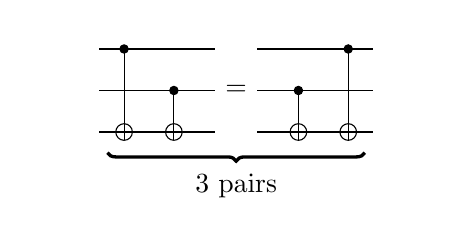
\begin{tikzpicture}[scale=1.000000,x=1pt,y=1pt]
\filldraw[color=white] (0.000000, -7.500000) rectangle (99.000000, 37.500000);
% Drawing wires
% Line 1: a1 W
\draw[color=black] (0.000000,30.000000) -- (99.000000,30.000000);
% Line 2: a2 W
\draw[color=black] (0.000000,15.000000) -- (99.000000,15.000000);
% Line 3: a3 W
\draw[color=black] (0.000000,0.000000) -- (99.000000,0.000000);
% Done with wires; drawing gates
% Line 4: a1 +a3
\draw (9.000000,30.000000) -- (9.000000,0.000000);
\filldraw (9.000000, 30.000000) circle(1.500000pt);
\begin{scope}
\draw[fill=white] (9.000000, 0.000000) circle(3.000000pt);
\clip (9.000000, 0.000000) circle(3.000000pt);
\draw (6.000000, 0.000000) -- (12.000000, 0.000000);
\draw (9.000000, -3.000000) -- (9.000000, 3.000000);
\end{scope}
% Line 5: a2 +a3
\draw (27.000000,15.000000) -- (27.000000,0.000000);
\filldraw (27.000000, 15.000000) circle(1.500000pt);
\begin{scope}
\draw[fill=white] (27.000000, 0.000000) circle(3.000000pt);
\clip (27.000000, 0.000000) circle(3.000000pt);
\draw (24.000000, 0.000000) -- (30.000000, 0.000000);
\draw (27.000000, -3.000000) -- (27.000000, 3.000000);
\end{scope}
% Line 6: =
\draw[fill=white,color=white] (42.000000, -6.000000) rectangle (57.000000, 36.000000);
\draw (49.500000, 15.000000) node {$=$};
% Line 7: a2 +a3
\draw (72.000000,15.000000) -- (72.000000,0.000000);
\filldraw (72.000000, 15.000000) circle(1.500000pt);
\begin{scope}
\draw[fill=white] (72.000000, 0.000000) circle(3.000000pt);
\clip (72.000000, 0.000000) circle(3.000000pt);
\draw (69.000000, 0.000000) -- (75.000000, 0.000000);
\draw (72.000000, -3.000000) -- (72.000000, 3.000000);
\end{scope}
% Line 8: a1 +a3
\draw (90.000000,30.000000) -- (90.000000,0.000000);
\filldraw (90.000000, 30.000000) circle(1.500000pt);
\begin{scope}
\draw[fill=white] (90.000000, 0.000000) circle(3.000000pt);
\clip (90.000000, 0.000000) circle(3.000000pt);
\draw (87.000000, 0.000000) -- (93.000000, 0.000000);
\draw (90.000000, -3.000000) -- (90.000000, 3.000000);
\end{scope}
% Done with gates; drawing ending labels
% Done with ending labels; drawing cut lines and comments
% Line 9: @ %% 3 pairs
\draw[decorate,decoration={brace,mirror,amplitude = 3.000000pt},very thick] (3.000000,-7.500000) -- (96.000000,-7.500000);
\draw (49.500000, -11.500000) node[text width=144pt,below,text centered] {3 pairs};
% Done with comments
\end{tikzpicture}
\end{center}
\vspace{-10pt}
\Textbf{4.28} For $U=V^2$ with $V$ unitary, construct a $C^5(U)$ gate analogous to that in Figure 4.10, but using no work qubits.  You may use controlled-$V$ and controlled-$V^\dagger$ gates.
\Soln NOTE: this task is only feasible if ``controlled-$V$ and controlled-$V^\dagger$ gates'' is interpreted to mean $C(V)$, $C(V^\dagger)$, \underline{and} $C^4(V)$, along with $C^4(X)$ gates. The $C^4(V)$ gate will implicitly require the existence of a unitary gate $W$ such that $W^2=V$ and the use of $C(W)$, $C(W^\dagger)$, $C^3(W)$ and $C^3(X)$ gates, which in turn require the existence of a unitary gate $P$ such that $P^2=W$ and the use of $C(P)$, $C(P^\dagger)$, $C^2(P)$ and $C^2(X)$ (Toffoli) gates.  Finally, the $C^2(P)$ gate requires the existence of unitary $Q$ such that $Q^2=P$ and the use of controlled-$Q$, controlled-$Q^\dagger$ along with $C(X)$ gates.  We'll construct $C^n(X)$ gates from Toffolis and 2-qubit gate in Exercise 4.29.  In Exercise 4.24 we constructed Toffoli gates from 2-qubit gates, but still, in order to execute a $C^n(U)$ using \underline{only} 1- and 2-qubit gates, we'd need a 1-qubit gate performing a unitary operator whose $2^n$-th power is $U$.  This gate may be guaranteed to exist theoretically, possibly under suitable hypotheses, but is almost certainly extremely difficult to implement physically.  So, a construction of such a circuit is of questionable value.  Instead, we offer a circuit using $C(V), C(V^\dagger)$ and $C^4(V)$.  The circuits using $C^3(W)$, $C^2(P)$, and $C(Q)$ can be constructed recursively in turn.  For a relatively rigorous mathematical proof of the infeasibility of the exercise without the use of $C^4(V)$-gates, see Wilfred Lee's answer to this cs.stackexchange question \href{_}\url{https://cs.stackexchange.com/questions/80538/is-it-possible-to-construct-a-c5u-with-v2-u-and-no-work-qubits-nielsen-ch}
\begin{center}
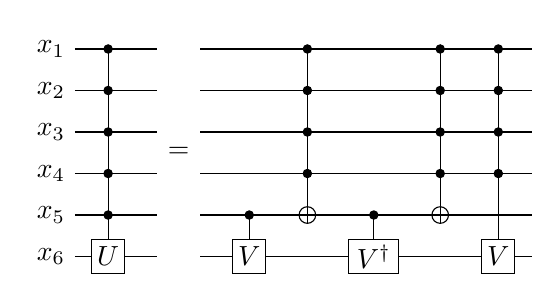
\begin{tikzpicture}[scale=1.000000,x=1pt,y=1pt]
\filldraw[color=white] (0.000000, -7.500000) rectangle (165.000000, 82.500000);
% Drawing wires
% Line 1: a1 W x_1
\draw[color=black] (0.000000,75.000000) -- (165.000000,75.000000);
\draw[color=black] (0.000000,75.000000) node[left] {$x_1$};
% Line 2: a2 W x_2
\draw[color=black] (0.000000,60.000000) -- (165.000000,60.000000);
\draw[color=black] (0.000000,60.000000) node[left] {$x_2$};
% Line 3: a3 W x_3
\draw[color=black] (0.000000,45.000000) -- (165.000000,45.000000);
\draw[color=black] (0.000000,45.000000) node[left] {$x_3$};
% Line 4: a4 W x_4
\draw[color=black] (0.000000,30.000000) -- (165.000000,30.000000);
\draw[color=black] (0.000000,30.000000) node[left] {$x_4$};
% Line 5: a5 W x_5
\draw[color=black] (0.000000,15.000000) -- (165.000000,15.000000);
\draw[color=black] (0.000000,15.000000) node[left] {$x_5$};
% Line 6: a6 W x_6
\draw[color=black] (0.000000,0.000000) -- (165.000000,0.000000);
\draw[color=black] (0.000000,0.000000) node[left] {$x_6$};
% Done with wires; drawing gates
% Line 7: a6 G $U$ a1 a2 a3 a4 a5
\draw (12.000000,75.000000) -- (12.000000,0.000000);
\begin{scope}
\draw[fill=white] (12.000000, -0.000000) +(-45.000000:8.485281pt and 8.485281pt) -- +(45.000000:8.485281pt and 8.485281pt) -- +(135.000000:8.485281pt and 8.485281pt) -- +(225.000000:8.485281pt and 8.485281pt) -- cycle;
\clip (12.000000, -0.000000) +(-45.000000:8.485281pt and 8.485281pt) -- +(45.000000:8.485281pt and 8.485281pt) -- +(135.000000:8.485281pt and 8.485281pt) -- +(225.000000:8.485281pt and 8.485281pt) -- cycle;
\draw (12.000000, -0.000000) node {$U$};
\end{scope}
\filldraw (12.000000, 75.000000) circle(1.500000pt);
\filldraw (12.000000, 60.000000) circle(1.500000pt);
\filldraw (12.000000, 45.000000) circle(1.500000pt);
\filldraw (12.000000, 30.000000) circle(1.500000pt);
\filldraw (12.000000, 15.000000) circle(1.500000pt);
% Line 8: =
\draw[fill=white,color=white] (30.000000, -6.000000) rectangle (45.000000, 81.000000);
\draw (37.500000, 37.500000) node {$=$};
% Line 9: a6 G $V$ a5
\draw (63.000000,15.000000) -- (63.000000,0.000000);
\begin{scope}
\draw[fill=white] (63.000000, -0.000000) +(-45.000000:8.485281pt and 8.485281pt) -- +(45.000000:8.485281pt and 8.485281pt) -- +(135.000000:8.485281pt and 8.485281pt) -- +(225.000000:8.485281pt and 8.485281pt) -- cycle;
\clip (63.000000, -0.000000) +(-45.000000:8.485281pt and 8.485281pt) -- +(45.000000:8.485281pt and 8.485281pt) -- +(135.000000:8.485281pt and 8.485281pt) -- +(225.000000:8.485281pt and 8.485281pt) -- cycle;
\draw (63.000000, -0.000000) node {$V$};
\end{scope}
\filldraw (63.000000, 15.000000) circle(1.500000pt);
% Line 10: a1 a2 a3 a4 +a5
\draw (84.000000,75.000000) -- (84.000000,15.000000);
\filldraw (84.000000, 75.000000) circle(1.500000pt);
\filldraw (84.000000, 60.000000) circle(1.500000pt);
\filldraw (84.000000, 45.000000) circle(1.500000pt);
\filldraw (84.000000, 30.000000) circle(1.500000pt);
\begin{scope}
\draw[fill=white] (84.000000, 15.000000) circle(3.000000pt);
\clip (84.000000, 15.000000) circle(3.000000pt);
\draw (81.000000, 15.000000) -- (87.000000, 15.000000);
\draw (84.000000, 12.000000) -- (84.000000, 18.000000);
\end{scope}
% Line 11: a6 G $V^\dagger$  a5 width=18
\draw (108.000000,15.000000) -- (108.000000,0.000000);
\begin{scope}
\draw[fill=white] (108.000000, -0.000000) +(-45.000000:12.727922pt and 8.485281pt) -- +(45.000000:12.727922pt and 8.485281pt) -- +(135.000000:12.727922pt and 8.485281pt) -- +(225.000000:12.727922pt and 8.485281pt) -- cycle;
\clip (108.000000, -0.000000) +(-45.000000:12.727922pt and 8.485281pt) -- +(45.000000:12.727922pt and 8.485281pt) -- +(135.000000:12.727922pt and 8.485281pt) -- +(225.000000:12.727922pt and 8.485281pt) -- cycle;
\draw (108.000000, -0.000000) node {$V^\dagger$};
\end{scope}
\filldraw (108.000000, 15.000000) circle(1.500000pt);
% Line 12: a1 a2 a3 a4 +a5
\draw (132.000000,75.000000) -- (132.000000,15.000000);
\filldraw (132.000000, 75.000000) circle(1.500000pt);
\filldraw (132.000000, 60.000000) circle(1.500000pt);
\filldraw (132.000000, 45.000000) circle(1.500000pt);
\filldraw (132.000000, 30.000000) circle(1.500000pt);
\begin{scope}
\draw[fill=white] (132.000000, 15.000000) circle(3.000000pt);
\clip (132.000000, 15.000000) circle(3.000000pt);
\draw (129.000000, 15.000000) -- (135.000000, 15.000000);
\draw (132.000000, 12.000000) -- (132.000000, 18.000000);
\end{scope}
% Line 13: a6 G $V$ a1 a2 a3 a4
\draw (153.000000,75.000000) -- (153.000000,0.000000);
\begin{scope}
\draw[fill=white] (153.000000, -0.000000) +(-45.000000:8.485281pt and 8.485281pt) -- +(45.000000:8.485281pt and 8.485281pt) -- +(135.000000:8.485281pt and 8.485281pt) -- +(225.000000:8.485281pt and 8.485281pt) -- cycle;
\clip (153.000000, -0.000000) +(-45.000000:8.485281pt and 8.485281pt) -- +(45.000000:8.485281pt and 8.485281pt) -- +(135.000000:8.485281pt and 8.485281pt) -- +(225.000000:8.485281pt and 8.485281pt) -- cycle;
\draw (153.000000, -0.000000) node {$V$};
\end{scope}
\filldraw (153.000000, 75.000000) circle(1.500000pt);
\filldraw (153.000000, 60.000000) circle(1.500000pt);
\filldraw (153.000000, 45.000000) circle(1.500000pt);
\filldraw (153.000000, 30.000000) circle(1.500000pt);
% Done with gates; drawing ending labels
% Done with ending labels; drawing cut lines and comments
% Done with comments
\end{tikzpicture}
\end{center}
\vspace{-10pt}
The verification of this circuit is identical to that of the circuit in figure 8 in Exercise 4.21, where instead of checking each computational basis state of $\ket{x_1}\ket{x_2}$, we check the states of $\ket{x_1x_2x_3x_4}\ket{x_5}$, where the possible states of $\ket{x_5}$ are the usual $\ket{0}$ and $\ket{1}$, but the states of $\ket{x_1x_2x_3x_4}$ are $\ket{1111}$ and $\neg\ket{1111}$, \textit{i.e.} anything other than $\ket{1111}$.

\Textbf{4.29} Find a circuit containing $O(n^2)$ Toffoli, \CNOT\ and single qubit gates which implements a $C^n(X)$ gate (for $n>3$), using no work qubits.
\Soln This exercise is also impossible as specified and interpreted naturally.
\begin{comment}  A succinct proof is offered by Craig Gidney in various placed, in particular here: \href{_}\url{https://algassert.com/circuits/2015/06/05/Constructing-Large-Controlled-Nots.html}.  We summarize
\end{comment}
\Textbf{4.30}
\Textbf{4.31} \textbf{(More circuit identities)}  Let subscripts denote which qubit an operator acts on, and let C be a \CNOT\ with qubit 1 the control and qubit 2 the target qubit.  Prove the following identities:
\begin{center}
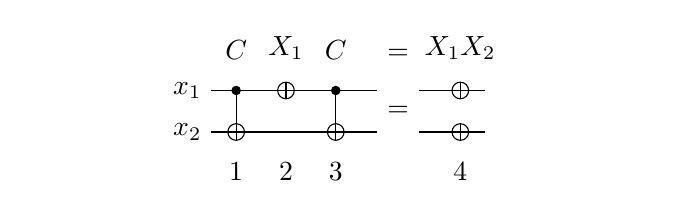
\begin{tikzpicture}[scale=1.000000,x=1pt,y=1pt]
\filldraw[color=white] (0.000000, -7.500000) rectangle (99.000000, 22.500000);
% Drawing wires
% Line 1: a1 W x_1
\draw[color=black] (0.000000,15.000000) -- (99.000000,15.000000);
\draw[color=black] (0.000000,15.000000) node[left] {$x_1$};
% Line 2: a2 W x_2
\draw[color=black] (0.000000,0.000000) -- (99.000000,0.000000);
\draw[color=black] (0.000000,0.000000) node[left] {$x_2$};
% Done with wires; drawing gates
% Line 3: a1 +a2 % $C$ % 1
\draw (9.000000, 22.500000) node[text width=144pt,above,text centered] {$C$};
\draw (9.000000, -7.500000) node[text width=144pt,below,text centered] {1};
\draw (9.000000,15.000000) -- (9.000000,0.000000);
\filldraw (9.000000, 15.000000) circle(1.500000pt);
\begin{scope}
\draw[fill=white] (9.000000, 0.000000) circle(3.000000pt);
\clip (9.000000, 0.000000) circle(3.000000pt);
\draw (6.000000, 0.000000) -- (12.000000, 0.000000);
\draw (9.000000, -3.000000) -- (9.000000, 3.000000);
\end{scope}
% Line 4: +a1 % $X_1$ % 2
\draw (27.000000, 22.500000) node[text width=144pt,above,text centered] {$X_1$};
\draw (27.000000, -7.500000) node[text width=144pt,below,text centered] {2};
\begin{scope}
\draw[fill=white] (27.000000, 15.000000) circle(3.000000pt);
\clip (27.000000, 15.000000) circle(3.000000pt);
\draw (24.000000, 15.000000) -- (30.000000, 15.000000);
\draw (27.000000, 12.000000) -- (27.000000, 18.000000);
\end{scope}
% Line 5: a1 +a2 % $C$ % 3
\draw (45.000000, 22.500000) node[text width=144pt,above,text centered] {$C$};
\draw (45.000000, -7.500000) node[text width=144pt,below,text centered] {3};
\draw (45.000000,15.000000) -- (45.000000,0.000000);
\filldraw (45.000000, 15.000000) circle(1.500000pt);
\begin{scope}
\draw[fill=white] (45.000000, 0.000000) circle(3.000000pt);
\clip (45.000000, 0.000000) circle(3.000000pt);
\draw (42.000000, 0.000000) -- (48.000000, 0.000000);
\draw (45.000000, -3.000000) -- (45.000000, 3.000000);
\end{scope}
% Line 6: = % =
\draw (67.500000, 22.500000) node[text width=144pt,above,text centered] {=};
\draw[fill=white,color=white] (60.000000, -6.000000) rectangle (75.000000, 21.000000);
\draw (67.500000, 7.500000) node {$=$};
% Line 7: +a1
\begin{scope}
\draw[fill=white] (90.000000, 15.000000) circle(3.000000pt);
\clip (90.000000, 15.000000) circle(3.000000pt);
\draw (87.000000, 15.000000) -- (93.000000, 15.000000);
\draw (90.000000, 12.000000) -- (90.000000, 18.000000);
\end{scope}
% Line 8: +a2  %$X_1X_2$ %  4
\draw (90.000000, 22.500000) node[text width=144pt,above,text centered] {$X_1X_2$};
\draw (90.000000, -7.500000) node[text width=144pt,below,text centered] {4};
\begin{scope}
\draw[fill=white] (90.000000, 0.000000) circle(3.000000pt);
\clip (90.000000, 0.000000) circle(3.000000pt);
\draw (87.000000, 0.000000) -- (93.000000, 0.000000);
\draw (90.000000, -3.000000) -- (90.000000, 3.000000);
\end{scope}
% Done with gates; drawing ending labels
% Done with ending labels; drawing cut lines and comments
% Done with comments
\end{tikzpicture}

\begin{tabular}{c|r|r|r||r} 
$\ket{x_1x_2}$ & \multicolumn{1}{c|}{1} & \multicolumn{1}{c|}{2} & \multicolumn{1}{c||}{3} & \multicolumn{1}{c}{4} \\
\hline
$\ket{00}$ & $\ket{00}$ & $\ket{10}$ & $\ket{11}$ & $\ket{11}$ \\
\hline
$\ket{01}$ & $\ket{01}$ & $\ket{11}$ & $\ket{10}$ & $\ket{10}$ \\
\hline
$\ket{10}$ & $\ket{11}$ & $\ket{01}$ & $\ket{01}$ & $\ket{01}$ \\
\hline
$\ket{11}$ & $\ket{10}$ & $\ket{00}$ & $\ket{00}$ & $\ket{00}$ \\
\end{tabular}
\end{center}
\noindent\rule{\textwidth}{1pt}
\begin{center}
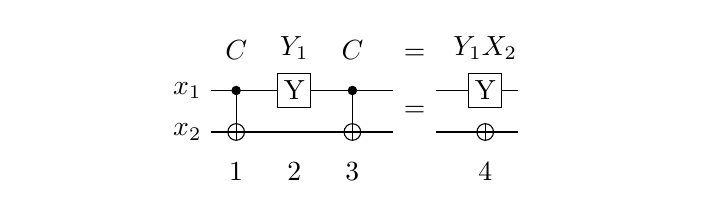
\begin{tikzpicture}[scale=1.000000,x=1pt,y=1pt]
\filldraw[color=white] (0.000000, -7.500000) rectangle (111.000000, 22.500000);
% Drawing wires
% Line 1: a1 W x_1
\draw[color=black] (0.000000,15.000000) -- (111.000000,15.000000);
\draw[color=black] (0.000000,15.000000) node[left] {$x_1$};
% Line 2: a2 W x_2
\draw[color=black] (0.000000,0.000000) -- (111.000000,0.000000);
\draw[color=black] (0.000000,0.000000) node[left] {$x_2$};
% Done with wires; drawing gates
% Line 3: a1 +a2 % $C$ % 1
\draw (9.000000, 22.500000) node[text width=144pt,above,text centered] {$C$};
\draw (9.000000, -7.500000) node[text width=144pt,below,text centered] {1};
\draw (9.000000,15.000000) -- (9.000000,0.000000);
\filldraw (9.000000, 15.000000) circle(1.500000pt);
\begin{scope}
\draw[fill=white] (9.000000, 0.000000) circle(3.000000pt);
\clip (9.000000, 0.000000) circle(3.000000pt);
\draw (6.000000, 0.000000) -- (12.000000, 0.000000);
\draw (9.000000, -3.000000) -- (9.000000, 3.000000);
\end{scope}
% Line 4: a1 G Y % $Y_1$ % 2
\draw (30.000000, 22.500000) node[text width=144pt,above,text centered] {$Y_1$};
\draw (30.000000, -7.500000) node[text width=144pt,below,text centered] {2};
\begin{scope}
\draw[fill=white] (30.000000, 15.000000) +(-45.000000:8.485281pt and 8.485281pt) -- +(45.000000:8.485281pt and 8.485281pt) -- +(135.000000:8.485281pt and 8.485281pt) -- +(225.000000:8.485281pt and 8.485281pt) -- cycle;
\clip (30.000000, 15.000000) +(-45.000000:8.485281pt and 8.485281pt) -- +(45.000000:8.485281pt and 8.485281pt) -- +(135.000000:8.485281pt and 8.485281pt) -- +(225.000000:8.485281pt and 8.485281pt) -- cycle;
\draw (30.000000, 15.000000) node {Y};
\end{scope}
% Line 5: a1 +a2 % $C$ % 3
\draw (51.000000, 22.500000) node[text width=144pt,above,text centered] {$C$};
\draw (51.000000, -7.500000) node[text width=144pt,below,text centered] {3};
\draw (51.000000,15.000000) -- (51.000000,0.000000);
\filldraw (51.000000, 15.000000) circle(1.500000pt);
\begin{scope}
\draw[fill=white] (51.000000, 0.000000) circle(3.000000pt);
\clip (51.000000, 0.000000) circle(3.000000pt);
\draw (48.000000, 0.000000) -- (54.000000, 0.000000);
\draw (51.000000, -3.000000) -- (51.000000, 3.000000);
\end{scope}
% Line 6: = % =
\draw (73.500000, 22.500000) node[text width=144pt,above,text centered] {=};
\draw[fill=white,color=white] (66.000000, -6.000000) rectangle (81.000000, 21.000000);
\draw (73.500000, 7.500000) node {$=$};
% Line 7: a1 G Y
\begin{scope}
\draw[fill=white] (99.000000, 15.000000) +(-45.000000:8.485281pt and 8.485281pt) -- +(45.000000:8.485281pt and 8.485281pt) -- +(135.000000:8.485281pt and 8.485281pt) -- +(225.000000:8.485281pt and 8.485281pt) -- cycle;
\clip (99.000000, 15.000000) +(-45.000000:8.485281pt and 8.485281pt) -- +(45.000000:8.485281pt and 8.485281pt) -- +(135.000000:8.485281pt and 8.485281pt) -- +(225.000000:8.485281pt and 8.485281pt) -- cycle;
\draw (99.000000, 15.000000) node {Y};
\end{scope}
% Line 8: +a2  %$Y_1X_2$ %  4
\draw (99.000000, 22.500000) node[text width=144pt,above,text centered] {$Y_1X_2$};
\draw (99.000000, -7.500000) node[text width=144pt,below,text centered] {4};
\begin{scope}
\draw[fill=white] (99.000000, 0.000000) circle(3.000000pt);
\clip (99.000000, 0.000000) circle(3.000000pt);
\draw (96.000000, 0.000000) -- (102.000000, 0.000000);
\draw (99.000000, -3.000000) -- (99.000000, 3.000000);
\end{scope}
% Done with gates; drawing ending labels
% Done with ending labels; drawing cut lines and comments
% Done with comments
\end{tikzpicture}

\begin{tabular}{c|r|r|r||r} 
$\ket{x_1x_2}$ & \multicolumn{1}{c|}{1} & \multicolumn{1}{c|}{2} & \multicolumn{1}{c||}{3} & \multicolumn{1}{c}{4} \\
\hline
$\ket{00}$ & $\ket{00}$ & $i\ket{10}$ & $i\ket{11}$ & $i\ket{11}$ \\
\hline
$\ket{01}$ & $\ket{01}$ & $i\ket{11}$ & $i\ket{10}$ & $i\ket{10}$ \\
\hline
$\ket{10}$ & $\ket{11}$ & $-i\ket{01}$ & $-i\ket{01}$ & $-i\ket{01}$ \\
\hline
$\ket{11}$ & $\ket{10}$ & $-i\ket{00}$ & $-i\ket{00}$ & $-i\ket{00}$ \\
\end{tabular}
\end{center}
\noindent\rule{\textwidth}{1pt}
\begin{center}
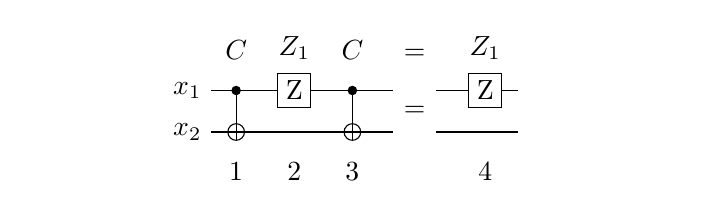
\begin{tikzpicture}[scale=1.000000,x=1pt,y=1pt]
\filldraw[color=white] (0.000000, -7.500000) rectangle (111.000000, 22.500000);
% Drawing wires
% Line 1: a1 W x_1
\draw[color=black] (0.000000,15.000000) -- (111.000000,15.000000);
\draw[color=black] (0.000000,15.000000) node[left] {$x_1$};
% Line 2: a2 W x_2
\draw[color=black] (0.000000,0.000000) -- (111.000000,0.000000);
\draw[color=black] (0.000000,0.000000) node[left] {$x_2$};
% Done with wires; drawing gates
% Line 3: a1 +a2 % $C$ % 1
\draw (9.000000, 22.500000) node[text width=144pt,above,text centered] {$C$};
\draw (9.000000, -7.500000) node[text width=144pt,below,text centered] {1};
\draw (9.000000,15.000000) -- (9.000000,0.000000);
\filldraw (9.000000, 15.000000) circle(1.500000pt);
\begin{scope}
\draw[fill=white] (9.000000, 0.000000) circle(3.000000pt);
\clip (9.000000, 0.000000) circle(3.000000pt);
\draw (6.000000, 0.000000) -- (12.000000, 0.000000);
\draw (9.000000, -3.000000) -- (9.000000, 3.000000);
\end{scope}
% Line 4: a1 G Z % $Z_1$ % 2
\draw (30.000000, 22.500000) node[text width=144pt,above,text centered] {$Z_1$};
\draw (30.000000, -7.500000) node[text width=144pt,below,text centered] {2};
\begin{scope}
\draw[fill=white] (30.000000, 15.000000) +(-45.000000:8.485281pt and 8.485281pt) -- +(45.000000:8.485281pt and 8.485281pt) -- +(135.000000:8.485281pt and 8.485281pt) -- +(225.000000:8.485281pt and 8.485281pt) -- cycle;
\clip (30.000000, 15.000000) +(-45.000000:8.485281pt and 8.485281pt) -- +(45.000000:8.485281pt and 8.485281pt) -- +(135.000000:8.485281pt and 8.485281pt) -- +(225.000000:8.485281pt and 8.485281pt) -- cycle;
\draw (30.000000, 15.000000) node {Z};
\end{scope}
% Line 5: a1 +a2 % $C$ % 3
\draw (51.000000, 22.500000) node[text width=144pt,above,text centered] {$C$};
\draw (51.000000, -7.500000) node[text width=144pt,below,text centered] {3};
\draw (51.000000,15.000000) -- (51.000000,0.000000);
\filldraw (51.000000, 15.000000) circle(1.500000pt);
\begin{scope}
\draw[fill=white] (51.000000, 0.000000) circle(3.000000pt);
\clip (51.000000, 0.000000) circle(3.000000pt);
\draw (48.000000, 0.000000) -- (54.000000, 0.000000);
\draw (51.000000, -3.000000) -- (51.000000, 3.000000);
\end{scope}
% Line 6: = % =
\draw (73.500000, 22.500000) node[text width=144pt,above,text centered] {=};
\draw[fill=white,color=white] (66.000000, -6.000000) rectangle (81.000000, 21.000000);
\draw (73.500000, 7.500000) node {$=$};
% Line 7: a1 G  Z %$Z_1$% 4
\draw (99.000000, 22.500000) node[text width=144pt,above,text centered] {$Z_1$};
\draw (99.000000, -7.500000) node[text width=144pt,below,text centered] {4};
\begin{scope}
\draw[fill=white] (99.000000, 15.000000) +(-45.000000:8.485281pt and 8.485281pt) -- +(45.000000:8.485281pt and 8.485281pt) -- +(135.000000:8.485281pt and 8.485281pt) -- +(225.000000:8.485281pt and 8.485281pt) -- cycle;
\clip (99.000000, 15.000000) +(-45.000000:8.485281pt and 8.485281pt) -- +(45.000000:8.485281pt and 8.485281pt) -- +(135.000000:8.485281pt and 8.485281pt) -- +(225.000000:8.485281pt and 8.485281pt) -- cycle;
\draw (99.000000, 15.000000) node {Z};
\end{scope}
% Done with gates; drawing ending labels
% Done with ending labels; drawing cut lines and comments
% Done with comments
\end{tikzpicture}

\begin{tabular}{c|r|r|r||r} 
$\ket{x_1x_2}$ & \multicolumn{1}{c|}{1} & \multicolumn{1}{c|}{2} & \multicolumn{1}{c||}{3} & \multicolumn{1}{c}{4} \\
\hline
$\ket{00}$ & $\ket{00}$ & $\ket{00}$ & $\ket{00}$ & $\ket{00}$ \\
\hline
$\ket{01}$ & $\ket{01}$ & $\ket{01}$ & $\ket{01}$ & $\ket{01}$ \\
\hline
$\ket{10}$ & $\ket{11}$ & $-\ket{11}$ & $-\ket{10}$ & $-\ket{10}$ \\
\hline
$\ket{11}$ & $\ket{10}$ & $-\ket{10}$ & $-\ket{11}$ & $-\ket{11}$ \\
\end{tabular}
\end{center}
\noindent\rule{\textwidth}{1pt}
\begin{center}
\begin{tikzpicture}[scale=1.000000,x=1pt,y=1pt]
\filldraw[color=white] (0.000000, -7.500000) rectangle (99.000000, 22.500000);
% Drawing wires
% Line 1: a1 W x_1
\draw[color=black] (0.000000,15.000000) -- (99.000000,15.000000);
\draw[color=black] (0.000000,15.000000) node[left] {$x_1$};
% Line 2: a2 W x_2
\draw[color=black] (0.000000,0.000000) -- (99.000000,0.000000);
\draw[color=black] (0.000000,0.000000) node[left] {$x_2$};
% Done with wires; drawing gates
% Line 3: a1 +a2 % $C$ % 1
\draw (9.000000, 22.500000) node[text width=144pt,above,text centered] {$C$};
\draw (9.000000, -7.500000) node[text width=144pt,below,text centered] {1};
\draw (9.000000,15.000000) -- (9.000000,0.000000);
\filldraw (9.000000, 15.000000) circle(1.500000pt);
\begin{scope}
\draw[fill=white] (9.000000, 0.000000) circle(3.000000pt);
\clip (9.000000, 0.000000) circle(3.000000pt);
\draw (6.000000, 0.000000) -- (12.000000, 0.000000);
\draw (9.000000, -3.000000) -- (9.000000, 3.000000);
\end{scope}
% Line 4: +a2  % $X_2$ % 2
\draw (27.000000, 22.500000) node[text width=144pt,above,text centered] {$X_2$};
\draw (27.000000, -7.500000) node[text width=144pt,below,text centered] {2};
\begin{scope}
\draw[fill=white] (27.000000, 0.000000) circle(3.000000pt);
\clip (27.000000, 0.000000) circle(3.000000pt);
\draw (24.000000, 0.000000) -- (30.000000, 0.000000);
\draw (27.000000, -3.000000) -- (27.000000, 3.000000);
\end{scope}
% Line 5: a1 +a2 % $C$ % 3
\draw (45.000000, 22.500000) node[text width=144pt,above,text centered] {$C$};
\draw (45.000000, -7.500000) node[text width=144pt,below,text centered] {3};
\draw (45.000000,15.000000) -- (45.000000,0.000000);
\filldraw (45.000000, 15.000000) circle(1.500000pt);
\begin{scope}
\draw[fill=white] (45.000000, 0.000000) circle(3.000000pt);
\clip (45.000000, 0.000000) circle(3.000000pt);
\draw (42.000000, 0.000000) -- (48.000000, 0.000000);
\draw (45.000000, -3.000000) -- (45.000000, 3.000000);
\end{scope}
% Line 6: = % =
\draw (67.500000, 22.500000) node[text width=144pt,above,text centered] {=};
\draw[fill=white,color=white] (60.000000, -6.000000) rectangle (75.000000, 21.000000);
\draw (67.500000, 7.500000) node {$=$};
% Line 7: +a2% $X_2$ % 4
\draw (90.000000, 22.500000) node[text width=144pt,above,text centered] {$X_2$};
\draw (90.000000, -7.500000) node[text width=144pt,below,text centered] {4};
\begin{scope}
\draw[fill=white] (90.000000, 0.000000) circle(3.000000pt);
\clip (90.000000, 0.000000) circle(3.000000pt);
\draw (87.000000, 0.000000) -- (93.000000, 0.000000);
\draw (90.000000, -3.000000) -- (90.000000, 3.000000);
\end{scope}
% Done with gates; drawing ending labels
% Done with ending labels; drawing cut lines and comments
% Done with comments
\end{tikzpicture}

\begin{tabular}{c|r|r|r||r} 
$\ket{x_1x_2}$ & \multicolumn{1}{c|}{1} & \multicolumn{1}{c|}{2} & \multicolumn{1}{c||}{3} & \multicolumn{1}{c}{4} \\
\hline
$\ket{00}$ & $\ket{00}$ & $\ket{01}$ & $\ket{01}$ & $\ket{01}$ \\
\hline
$\ket{01}$ & $\ket{01}$ & $\ket{00}$ & $\ket{00}$ & $\ket{00}$ \\
\hline
$\ket{10}$ & $\ket{11}$ & $\ket{10}$ & $\ket{11}$ & $\ket{11}$ \\
\hline
$\ket{11}$ & $\ket{10}$ & $\ket{11}$ & $\ket{10}$ & $\ket{10}$ \\
\end{tabular}
\end{center}
\noindent\rule{\textwidth}{1pt}
\begin{center}
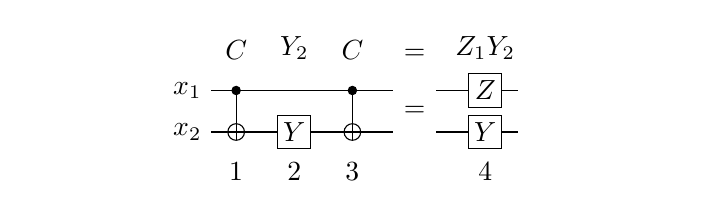
\begin{tikzpicture}[scale=1.000000,x=1pt,y=1pt]
\filldraw[color=white] (0.000000, -7.500000) rectangle (111.000000, 22.500000);
% Drawing wires
% Line 1: a1 W x_1
\draw[color=black] (0.000000,15.000000) -- (111.000000,15.000000);
\draw[color=black] (0.000000,15.000000) node[left] {$x_1$};
% Line 2: a2 W x_2
\draw[color=black] (0.000000,0.000000) -- (111.000000,0.000000);
\draw[color=black] (0.000000,0.000000) node[left] {$x_2$};
% Done with wires; drawing gates
% Line 3: a1 +a2 % $C$ % 1
\draw (9.000000, 22.500000) node[text width=144pt,above,text centered] {$C$};
\draw (9.000000, -7.500000) node[text width=144pt,below,text centered] {1};
\draw (9.000000,15.000000) -- (9.000000,0.000000);
\filldraw (9.000000, 15.000000) circle(1.500000pt);
\begin{scope}
\draw[fill=white] (9.000000, 0.000000) circle(3.000000pt);
\clip (9.000000, 0.000000) circle(3.000000pt);
\draw (6.000000, 0.000000) -- (12.000000, 0.000000);
\draw (9.000000, -3.000000) -- (9.000000, 3.000000);
\end{scope}
% Line 4: a2 G $Y$ % $Y_1$ % 2
\draw (30.000000, 22.500000) node[text width=144pt,above,text centered] {$Y_2$};
\draw (30.000000, -7.500000) node[text width=144pt,below,text centered] {2};
\begin{scope}
\draw[fill=white] (30.000000, -0.000000) +(-45.000000:8.485281pt and 8.485281pt) -- +(45.000000:8.485281pt and 8.485281pt) -- +(135.000000:8.485281pt and 8.485281pt) -- +(225.000000:8.485281pt and 8.485281pt) -- cycle;
\clip (30.000000, -0.000000) +(-45.000000:8.485281pt and 8.485281pt) -- +(45.000000:8.485281pt and 8.485281pt) -- +(135.000000:8.485281pt and 8.485281pt) -- +(225.000000:8.485281pt and 8.485281pt) -- cycle;
\draw (30.000000, -0.000000) node {$Y$};
\end{scope}
% Line 5: a1 +a2 % $C$ % 3
\draw (51.000000, 22.500000) node[text width=144pt,above,text centered] {$C$};
\draw (51.000000, -7.500000) node[text width=144pt,below,text centered] {3};
\draw (51.000000,15.000000) -- (51.000000,0.000000);
\filldraw (51.000000, 15.000000) circle(1.500000pt);
\begin{scope}
\draw[fill=white] (51.000000, 0.000000) circle(3.000000pt);
\clip (51.000000, 0.000000) circle(3.000000pt);
\draw (48.000000, 0.000000) -- (54.000000, 0.000000);
\draw (51.000000, -3.000000) -- (51.000000, 3.000000);
\end{scope}
% Line 6: = % =
\draw (73.500000, 22.500000) node[text width=144pt,above,text centered] {=};
\draw[fill=white,color=white] (66.000000, -6.000000) rectangle (81.000000, 21.000000);
\draw (73.500000, 7.500000) node {$=$};
% Line 7: a1 G  $Z$  %$Z_1Y_2$% 4
\draw (99.000000, 22.500000) node[text width=144pt,above,text centered] {$Z_1Y_2$};
\draw (99.000000, -7.500000) node[text width=144pt,below,text centered] {4};
\begin{scope}
\draw[fill=white] (99.000000, 15.000000) +(-45.000000:8.485281pt and 8.485281pt) -- +(45.000000:8.485281pt and 8.485281pt) -- +(135.000000:8.485281pt and 8.485281pt) -- +(225.000000:8.485281pt and 8.485281pt) -- cycle;
\clip (99.000000, 15.000000) +(-45.000000:8.485281pt and 8.485281pt) -- +(45.000000:8.485281pt and 8.485281pt) -- +(135.000000:8.485281pt and 8.485281pt) -- +(225.000000:8.485281pt and 8.485281pt) -- cycle;
\draw (99.000000, 15.000000) node {$Z$};
\end{scope}
% Line 8: a2 G $Y$
\begin{scope}
\draw[fill=white] (99.000000, -0.000000) +(-45.000000:8.485281pt and 8.485281pt) -- +(45.000000:8.485281pt and 8.485281pt) -- +(135.000000:8.485281pt and 8.485281pt) -- +(225.000000:8.485281pt and 8.485281pt) -- cycle;
\clip (99.000000, -0.000000) +(-45.000000:8.485281pt and 8.485281pt) -- +(45.000000:8.485281pt and 8.485281pt) -- +(135.000000:8.485281pt and 8.485281pt) -- +(225.000000:8.485281pt and 8.485281pt) -- cycle;
\draw (99.000000, -0.000000) node {$Y$};
\end{scope}
% Done with gates; drawing ending labels
% Done with ending labels; drawing cut lines and comments
% Done with comments
\end{tikzpicture}

\begin{tabular}{c|r|r|r||r} 
$\ket{x_1x_2}$ & \multicolumn{1}{c|}{1} & \multicolumn{1}{c|}{2} & \multicolumn{1}{c||}{3} & \multicolumn{1}{c}{4} \\
\hline
$\ket{00}$ & $\ket{00}$ & $i\ket{01}$ & $i\ket{01}$ & $i\ket{01}$ \\
\hline
$\ket{01}$ & $\ket{01}$ & $-i\ket{00}$ & $-i\ket{00}$ & $-i\ket{00}$ \\
\hline
$\ket{10}$ & $\ket{11}$ & $-i\ket{10}$ & $-i\ket{11}$ & $-i\ket{11}$ \\
\hline
$\ket{11}$ & $\ket{10}$ & $i\ket{11}$ & $i\ket{10}$ & $i\ket{10}$ \\
\end{tabular}
\end{center}

\begin{center}
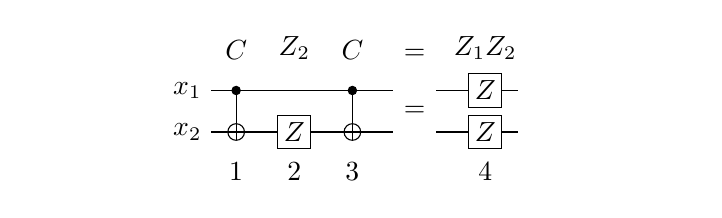
\begin{tikzpicture}[scale=1.000000,x=1pt,y=1pt]
\filldraw[color=white] (0.000000, -7.500000) rectangle (111.000000, 22.500000);
% Drawing wires
% Line 1: a1 W x_1
\draw[color=black] (0.000000,15.000000) -- (111.000000,15.000000);
\draw[color=black] (0.000000,15.000000) node[left] {$x_1$};
% Line 2: a2 W x_2
\draw[color=black] (0.000000,0.000000) -- (111.000000,0.000000);
\draw[color=black] (0.000000,0.000000) node[left] {$x_2$};
% Done with wires; drawing gates
% Line 3: a1 +a2 % $C$ % 1
\draw (9.000000, 22.500000) node[text width=144pt,above,text centered] {$C$};
\draw (9.000000, -7.500000) node[text width=144pt,below,text centered] {1};
\draw (9.000000,15.000000) -- (9.000000,0.000000);
\filldraw (9.000000, 15.000000) circle(1.500000pt);
\begin{scope}
\draw[fill=white] (9.000000, 0.000000) circle(3.000000pt);
\clip (9.000000, 0.000000) circle(3.000000pt);
\draw (6.000000, 0.000000) -- (12.000000, 0.000000);
\draw (9.000000, -3.000000) -- (9.000000, 3.000000);
\end{scope}
% Line 4: a2 G $Z$ % $Z_2$ % 2
\draw (30.000000, 22.500000) node[text width=144pt,above,text centered] {$Z_2$};
\draw (30.000000, -7.500000) node[text width=144pt,below,text centered] {2};
\begin{scope}
\draw[fill=white] (30.000000, -0.000000) +(-45.000000:8.485281pt and 8.485281pt) -- +(45.000000:8.485281pt and 8.485281pt) -- +(135.000000:8.485281pt and 8.485281pt) -- +(225.000000:8.485281pt and 8.485281pt) -- cycle;
\clip (30.000000, -0.000000) +(-45.000000:8.485281pt and 8.485281pt) -- +(45.000000:8.485281pt and 8.485281pt) -- +(135.000000:8.485281pt and 8.485281pt) -- +(225.000000:8.485281pt and 8.485281pt) -- cycle;
\draw (30.000000, -0.000000) node {$Z$};
\end{scope}
% Line 5: a1 +a2 % $C$ % 3
\draw (51.000000, 22.500000) node[text width=144pt,above,text centered] {$C$};
\draw (51.000000, -7.500000) node[text width=144pt,below,text centered] {3};
\draw (51.000000,15.000000) -- (51.000000,0.000000);
\filldraw (51.000000, 15.000000) circle(1.500000pt);
\begin{scope}
\draw[fill=white] (51.000000, 0.000000) circle(3.000000pt);
\clip (51.000000, 0.000000) circle(3.000000pt);
\draw (48.000000, 0.000000) -- (54.000000, 0.000000);
\draw (51.000000, -3.000000) -- (51.000000, 3.000000);
\end{scope}
% Line 6: = % =
\draw (73.500000, 22.500000) node[text width=144pt,above,text centered] {=};
\draw[fill=white,color=white] (66.000000, -6.000000) rectangle (81.000000, 21.000000);
\draw (73.500000, 7.500000) node {$=$};
% Line 7: a1 G  $Z$  %$Z_1Z_2$% 4
\draw (99.000000, 22.500000) node[text width=144pt,above,text centered] {$Z_1Z_2$};
\draw (99.000000, -7.500000) node[text width=144pt,below,text centered] {4};
\begin{scope}
\draw[fill=white] (99.000000, 15.000000) +(-45.000000:8.485281pt and 8.485281pt) -- +(45.000000:8.485281pt and 8.485281pt) -- +(135.000000:8.485281pt and 8.485281pt) -- +(225.000000:8.485281pt and 8.485281pt) -- cycle;
\clip (99.000000, 15.000000) +(-45.000000:8.485281pt and 8.485281pt) -- +(45.000000:8.485281pt and 8.485281pt) -- +(135.000000:8.485281pt and 8.485281pt) -- +(225.000000:8.485281pt and 8.485281pt) -- cycle;
\draw (99.000000, 15.000000) node {$Z$};
\end{scope}
% Line 8: a2 G $Z$
\begin{scope}
\draw[fill=white] (99.000000, -0.000000) +(-45.000000:8.485281pt and 8.485281pt) -- +(45.000000:8.485281pt and 8.485281pt) -- +(135.000000:8.485281pt and 8.485281pt) -- +(225.000000:8.485281pt and 8.485281pt) -- cycle;
\clip (99.000000, -0.000000) +(-45.000000:8.485281pt and 8.485281pt) -- +(45.000000:8.485281pt and 8.485281pt) -- +(135.000000:8.485281pt and 8.485281pt) -- +(225.000000:8.485281pt and 8.485281pt) -- cycle;
\draw (99.000000, -0.000000) node {$Z$};
\end{scope}
% Done with gates; drawing ending labels
% Done with ending labels; drawing cut lines and comments
% Done with comments
\end{tikzpicture}

\begin{tabular}{c|r|r|r||r} 
$\ket{x_1x_2}$ & \multicolumn{1}{c|}{1} & \multicolumn{1}{c|}{2} & \multicolumn{1}{c||}{3} & \multicolumn{1}{c}{4} \\
\hline
$\ket{00}$ & $\ket{00}$ & $\ket{00}$ & $\ket{00}$ & $\ket{00}$ \\
\hline
$\ket{01}$ & $\ket{01}$ & $-\ket{01}$ & $-\ket{01}$ & $-\ket{01}$ \\
\hline
$\ket{10}$ & $\ket{11}$ & $-\ket{11}$ & $-\ket{10}$ & $-\ket{10}$ \\
\hline
$\ket{11}$ & $\ket{10}$ & $\ket{10}$ & $\ket{11}$ & $\ket{11}$ \\
\end{tabular}
\end{center}
\noindent\rule{\textwidth}{1pt}
\begin{center}
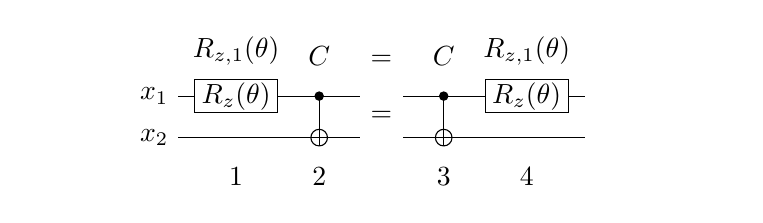
\begin{tikzpicture}[scale=1.000000,x=1pt,y=1pt]
\filldraw[color=white] (0.000000, -7.500000) rectangle (147.000000, 22.500000);
% Drawing wires
% Line 1: a1 W x_1
\draw[color=black] (0.000000,15.000000) -- (147.000000,15.000000);
\draw[color=black] (0.000000,15.000000) node[left] {$x_1$};
% Line 2: a2 W x_2
\draw[color=black] (0.000000,0.000000) -- (147.000000,0.000000);
\draw[color=black] (0.000000,0.000000) node[left] {$x_2$};
% Done with wires; drawing gates
% Line 3: a1 G $R_z(\theta)$ width=30%$R_{z,1}(\theta)$ % 1
\draw (21.000000, 22.500000) node[text width=144pt,above,text centered] {$R_{z,1}(\theta)$};
\draw (21.000000, -7.500000) node[text width=144pt,below,text centered] {1};
\begin{scope}
\draw[fill=white] (21.000000, 15.000000) +(-45.000000:21.213203pt and 8.485281pt) -- +(45.000000:21.213203pt and 8.485281pt) -- +(135.000000:21.213203pt and 8.485281pt) -- +(225.000000:21.213203pt and 8.485281pt) -- cycle;
\clip (21.000000, 15.000000) +(-45.000000:21.213203pt and 8.485281pt) -- +(45.000000:21.213203pt and 8.485281pt) -- +(135.000000:21.213203pt and 8.485281pt) -- +(225.000000:21.213203pt and 8.485281pt) -- cycle;
\draw (21.000000, 15.000000) node {$R_z(\theta)$};
\end{scope}
% Line 4: a1 +a2 % $C$ % 2
\draw (51.000000, 22.500000) node[text width=144pt,above,text centered] {$C$};
\draw (51.000000, -7.500000) node[text width=144pt,below,text centered] {2};
\draw (51.000000,15.000000) -- (51.000000,0.000000);
\filldraw (51.000000, 15.000000) circle(1.500000pt);
\begin{scope}
\draw[fill=white] (51.000000, 0.000000) circle(3.000000pt);
\clip (51.000000, 0.000000) circle(3.000000pt);
\draw (48.000000, 0.000000) -- (54.000000, 0.000000);
\draw (51.000000, -3.000000) -- (51.000000, 3.000000);
\end{scope}
% Line 5: = % $=$
\draw (73.500000, 22.500000) node[text width=144pt,above,text centered] {$=$};
\draw[fill=white,color=white] (66.000000, -6.000000) rectangle (81.000000, 21.000000);
\draw (73.500000, 7.500000) node {$=$};
% Line 6: a1 +a2 % $C$ % 3
\draw (96.000000, 22.500000) node[text width=144pt,above,text centered] {$C$};
\draw (96.000000, -7.500000) node[text width=144pt,below,text centered] {3};
\draw (96.000000,15.000000) -- (96.000000,0.000000);
\filldraw (96.000000, 15.000000) circle(1.500000pt);
\begin{scope}
\draw[fill=white] (96.000000, 0.000000) circle(3.000000pt);
\clip (96.000000, 0.000000) circle(3.000000pt);
\draw (93.000000, 0.000000) -- (99.000000, 0.000000);
\draw (96.000000, -3.000000) -- (96.000000, 3.000000);
\end{scope}
% Line 7: a1 G $R_z(\theta)$ width=30%$R_{z,1}(\theta)$ % 4
\draw (126.000000, 22.500000) node[text width=144pt,above,text centered] {$R_{z,1}(\theta)$};
\draw (126.000000, -7.500000) node[text width=144pt,below,text centered] {4};
\begin{scope}
\draw[fill=white] (126.000000, 15.000000) +(-45.000000:21.213203pt and 8.485281pt) -- +(45.000000:21.213203pt and 8.485281pt) -- +(135.000000:21.213203pt and 8.485281pt) -- +(225.000000:21.213203pt and 8.485281pt) -- cycle;
\clip (126.000000, 15.000000) +(-45.000000:21.213203pt and 8.485281pt) -- +(45.000000:21.213203pt and 8.485281pt) -- +(135.000000:21.213203pt and 8.485281pt) -- +(225.000000:21.213203pt and 8.485281pt) -- cycle;
\draw (126.000000, 15.000000) node {$R_z(\theta)$};
\end{scope}
% Done with gates; drawing ending labels
% Done with ending labels; drawing cut lines and comments
% Done with comments
\end{tikzpicture}

\begin{tabular}{c|r|r||r|r} 
$\ket{x_1x_2}$ & \multicolumn{1}{c|}{1} & \multicolumn{1}{c||}{2} & \multicolumn{1}{c|}{3} & \multicolumn{1}{c}{4} \\
\hline
$\ket{00}$ & $e^{-i\theta/2}\ket{00}$ & $e^{-i\theta/2}\ket{00}$ & $\ket{00}$ & $e^{-i\theta/2}\ket{00}$ \\
\hline
$\ket{01}$ & $e^{-i\theta/2}\ket{01}$ & $e^{-i\theta/2}\ket{01}$ & $\ket{01}$ & $e^{-i\theta/2}\ket{01}$ \\
\hline
$\ket{10}$ & $e^{i\theta/2}\ket{10}$ & $e^{i\theta/2}\ket{11}$ & $\ket{11}$ & $e^{i\theta/2}\ket{11}$ \\
\hline
$\ket{11}$ & $e^{i\theta/2}\ket{11}$ & $e^{i\theta/2}\ket{10}$ & $\ket{10}$ & $e^{i\theta/2}\ket{10}$ \\
\end{tabular}
\end{center}
\noindent\rule{\textwidth}{1pt}
\begin{center}
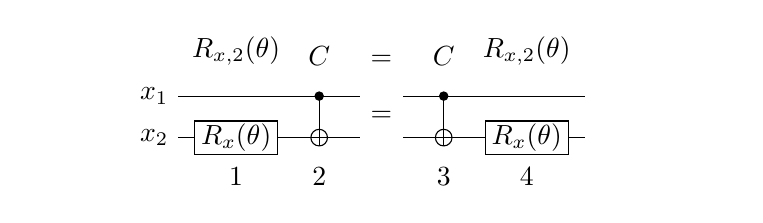
\begin{tikzpicture}[scale=1.000000,x=1pt,y=1pt]
\filldraw[color=white] (0.000000, -7.500000) rectangle (147.000000, 22.500000);
% Drawing wires
% Line 1: a1 W x_1
\draw[color=black] (0.000000,15.000000) -- (147.000000,15.000000);
\draw[color=black] (0.000000,15.000000) node[left] {$x_1$};
% Line 2: a2 W x_2
\draw[color=black] (0.000000,0.000000) -- (147.000000,0.000000);
\draw[color=black] (0.000000,0.000000) node[left] {$x_2$};
% Done with wires; drawing gates
% Line 3: a2 G $R_x(\theta)$ width=30%$R_{x,2}(\theta)$ % 1
\draw (21.000000, 22.500000) node[text width=144pt,above,text centered] {$R_{x,2}(\theta)$};
\draw (21.000000, -7.500000) node[text width=144pt,below,text centered] {1};
\begin{scope}
\draw[fill=white] (21.000000, -0.000000) +(-45.000000:21.213203pt and 8.485281pt) -- +(45.000000:21.213203pt and 8.485281pt) -- +(135.000000:21.213203pt and 8.485281pt) -- +(225.000000:21.213203pt and 8.485281pt) -- cycle;
\clip (21.000000, -0.000000) +(-45.000000:21.213203pt and 8.485281pt) -- +(45.000000:21.213203pt and 8.485281pt) -- +(135.000000:21.213203pt and 8.485281pt) -- +(225.000000:21.213203pt and 8.485281pt) -- cycle;
\draw (21.000000, -0.000000) node {$R_x(\theta)$};
\end{scope}
% Line 4: a1 +a2 % $C$ % 2
\draw (51.000000, 22.500000) node[text width=144pt,above,text centered] {$C$};
\draw (51.000000, -7.500000) node[text width=144pt,below,text centered] {2};
\draw (51.000000,15.000000) -- (51.000000,0.000000);
\filldraw (51.000000, 15.000000) circle(1.500000pt);
\begin{scope}
\draw[fill=white] (51.000000, 0.000000) circle(3.000000pt);
\clip (51.000000, 0.000000) circle(3.000000pt);
\draw (48.000000, 0.000000) -- (54.000000, 0.000000);
\draw (51.000000, -3.000000) -- (51.000000, 3.000000);
\end{scope}
% Line 5: = % $=$
\draw (73.500000, 22.500000) node[text width=144pt,above,text centered] {$=$};
\draw[fill=white,color=white] (66.000000, -6.000000) rectangle (81.000000, 21.000000);
\draw (73.500000, 7.500000) node {$=$};
% Line 6: a1 +a2 % $C$ % 3
\draw (96.000000, 22.500000) node[text width=144pt,above,text centered] {$C$};
\draw (96.000000, -7.500000) node[text width=144pt,below,text centered] {3};
\draw (96.000000,15.000000) -- (96.000000,0.000000);
\filldraw (96.000000, 15.000000) circle(1.500000pt);
\begin{scope}
\draw[fill=white] (96.000000, 0.000000) circle(3.000000pt);
\clip (96.000000, 0.000000) circle(3.000000pt);
\draw (93.000000, 0.000000) -- (99.000000, 0.000000);
\draw (96.000000, -3.000000) -- (96.000000, 3.000000);
\end{scope}
% Line 7: a2 G $R_x(\theta)$ width=30%$R_{x,2}(\theta)$ % 4
\draw (126.000000, 22.500000) node[text width=144pt,above,text centered] {$R_{x,2}(\theta)$};
\draw (126.000000, -7.500000) node[text width=144pt,below,text centered] {4};
\begin{scope}
\draw[fill=white] (126.000000, -0.000000) +(-45.000000:21.213203pt and 8.485281pt) -- +(45.000000:21.213203pt and 8.485281pt) -- +(135.000000:21.213203pt and 8.485281pt) -- +(225.000000:21.213203pt and 8.485281pt) -- cycle;
\clip (126.000000, -0.000000) +(-45.000000:21.213203pt and 8.485281pt) -- +(45.000000:21.213203pt and 8.485281pt) -- +(135.000000:21.213203pt and 8.485281pt) -- +(225.000000:21.213203pt and 8.485281pt) -- cycle;
\draw (126.000000, -0.000000) node {$R_x(\theta)$};
\end{scope}
% Done with gates; drawing ending labels
% Done with ending labels; drawing cut lines and comments
% Done with comments
\end{tikzpicture}

\begin{tabular}{c|r|r} 
$\ket{x_1x_2}$ & \multicolumn{1}{c|}{1} & \multicolumn{1}{c}{2} \\
\hline
$\ket{00}$ & $\cos(\theta/2)\ket{00}-i\sin(\theta/2)\ket{01}$ & $\cos(\theta/2)\ket{00}-i\sin(\theta/2)\ket{01}$ \\
\hline
$\ket{01}$ & $-i\sin(\theta/2)\ket{00}+\cos(\theta/2)\ket{01}$ & $-i\sin(\theta/2)\ket{00}+\cos(\theta/2)\ket{01}$ \\
\hline
$\ket{10}$ & $\cos(\theta/2)\ket{10}-i\sin(\theta/2)\ket{11}$ & $-i\sin(\theta/2)\ket{10}+\cos(\theta/2)\ket{11}$ \\
\hline
$\ket{11}$ & $-i\sin(\theta/2)\ket{10}+\cos(\theta/2)\ket{11}$ & $\cos(\theta/2)\ket{10}-i\sin(\theta/2)\ket{11}$ \\
\end{tabular}

\hspace{127.5pt}\begin{tabular}{c|r|r} 
$\ket{x_1x_2}$ & \multicolumn{1}{c|}{3} & \multicolumn{1}{c}{4} \\
\hline
$\ket{00}$ & $\ket{00}$ & $\cos(\theta/2)\ket{00}-i\sin(\theta/2)\ket{01}$ \\
\hline
$\ket{01}$ & $\ket{01}$ & $-i\sin(\theta/2)\ket{00}+\cos(\theta/2)\ket{01}$ \\
\hline
$\ket{10}$ & $\ket{11}$ & $-i\sin(\theta/2)\ket{10}+\cos(\theta/2)\ket{11}$ \\
\hline
$\ket{11}$ & $\ket{10}$ & $\cos(\theta/2)\ket{10}-i\sin(\theta/2)\ket{11}$ \\
\end{tabular}
\end{center}


